\section{The data-driven four-body mass background determination}
\label{sec:wjetsBackground}

\subsection{Background shapes for the four-body mass spectrum}
\label{sec:4bshapes}

Parameterizations for the background shapes are also determined for
events in the signal region for the WW mass spectrum.  The functional
form of the background is determined from MC and validated using the
data from the $m_{jj}$ sideband.  There are no peaking backgrounds in
the $m_{\ell\nu jj}$ spectrum which is dominated by W+jets production.

To validate the $m_{\ell\nu jj}$ W+jets shape we take the following
steps:

\begin{enumerate}
\item Fit the MC spectrum in the $m_{jj}$ signal region with the
  selected functional form.  If the $P(\chi^2) < 0.001$ then the
  functional form is rejected in favor of one with more degrees of
  freedom.
\item Fit the MC spectrum in the $m_{jj}$ sideband with the selected
  functional form.  Same criteria as step 1.
\item Fit the data spectrum in the $m_{jj}$ sideband.  Same criteria
  as step 1.
\item Fit the MC spectrum with a polynomial function with sufficient
  degrees of freedom to saturate the $\chi^2$ probability.
\item Compare the background estimate from the nominal functional form
  with that of the polynomial.  If the variation isn't well within the
  statistical error from of the nominal parameters reject the function
  in favor of one with more degrees of freedom.
\end{enumerate}

This procedure is repeated for each mass point under consideration.
The functional form varies by mass point.  The results of this test
are summarized in Table~\ref{tab:wjetsShapes}.  In the fit to the
data, the initial parameter values for the chosen functional form are
those determined from the MC.  These are nuisance parameters to the
limit extraction and are subjected to loose constraints based on the
MC shapes, but the ultimate values of the background shape nuisance
parameters are determined during the limit extraction minimization.

\begin{table}
  \caption{\label{tab:wjetsShapes} Results of the selection procedure
    to select a V+jets shape to use as the model for the $m_{\ell\nu jj}$ 
    spectrum.  The Bkg. rel. diff. is the relative differnece in background 
    normalization in the area of the Higgs peak from the nominal model 
    and the polynomial model.  The Bkg. diff. signif. is the significance 
    of this differnece with respect to the statistical variations of the 
    nominal model.}
\begin{center}
\begin{tabular}{ccccc}
\hline
Higgs mass & Nominal $m_{\ell\nu jj}$ shape & poly. order & Bkg. rel. diff. & Bkg diff. signif. \\
\hline
170 & erf*power &      4 & -0.0056 & 0.194 \\
180 & erf*exp &        4 &  0.0011 & 0.289 \\
190 & erf*exp &        4 &  0.0001 & 0.033 \\
200 & erf*power &      4 & -0.0004 & 0.118 \\
250 & erf*power &      4 & -0.0001 & 0.040 \\
300 & erf*power &      4 & -0.0013 & 0.448 \\
350 & exp(quadratic) & 4 &  0.0006 & 0.240 \\
400 & exp(quadratic) & 4 &  0.0035 & 0.473 \\
450 & power &          5 & -0.0016 & 0.302 \\
500 & power &          5 &  0.0011 & 0.193 \\
550 & power &          5 &  0.0026 & 0.464 \\
600 & power &          5 &  0.0020 & 0.377 \\
\hline
\end{tabular}
\end{center}
\end{table}

\subsection{Fit validation}
\label{sec:mlvjjvalidation}

We validate our fitting procedure using an ensemble of pseudo-data
experiments thrown from the nominal signal and background models.  We
consider the cases of $0\times$, $1\times$ and $2\times$ the SM for
the amount of Higgs signal included in each pseudo-data experiment.
We restrict our validation to the 180 GeV, 200 GeV, 300 GeV, 400 GeV
and 600 GeV mass points as these cover all of our various fitting
configurations.  The pull distributions for the signal strength
parameter $r$ are shown in
Figs.~\ref{fig:validation0}-\ref{fig:validation2}.  In all cases the
bias is negligible and we find that the errors returned by the ML fit
are conservative.

\begin{figure}
\begin{center}
  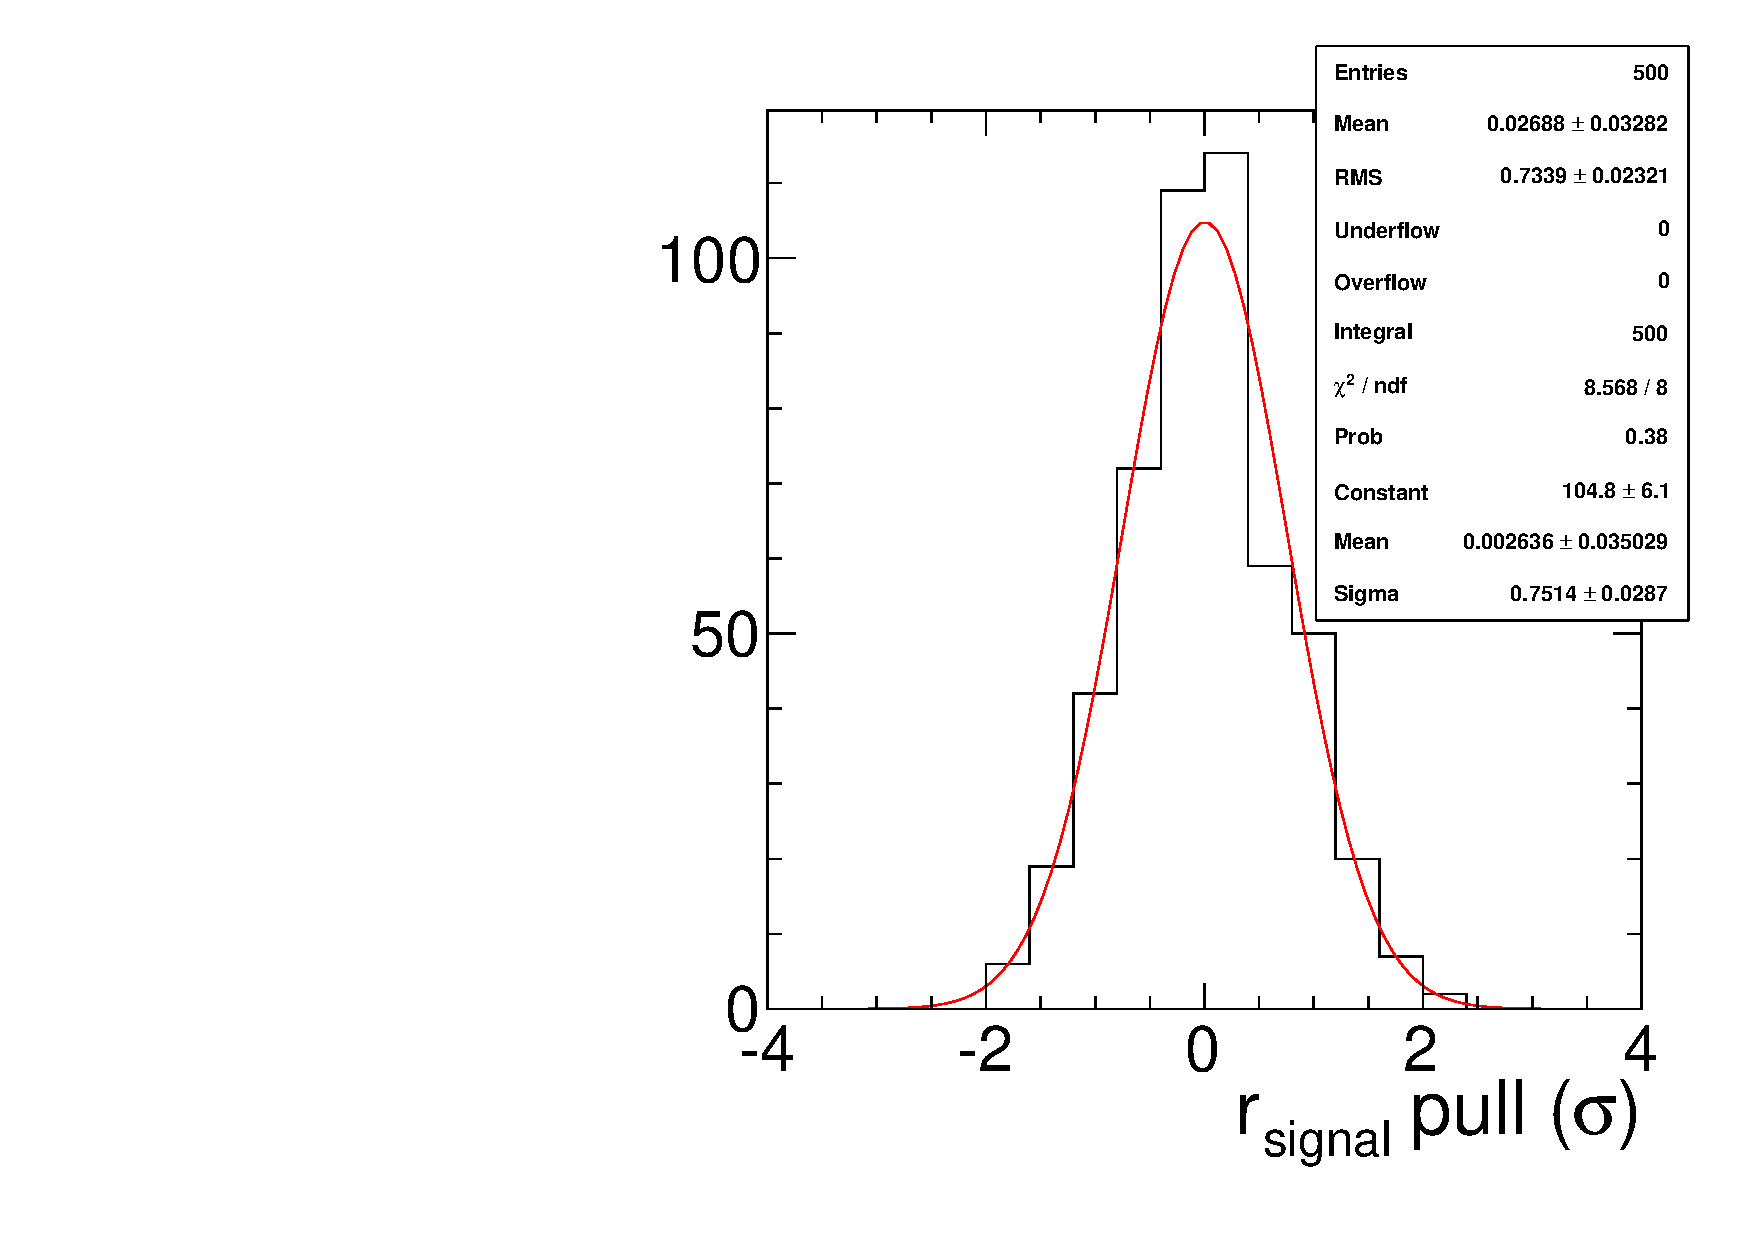
\includegraphics[width=0.4\textwidth]{plots/ML_validation/HWW180_Sig0_0_ToyResults_pull}
  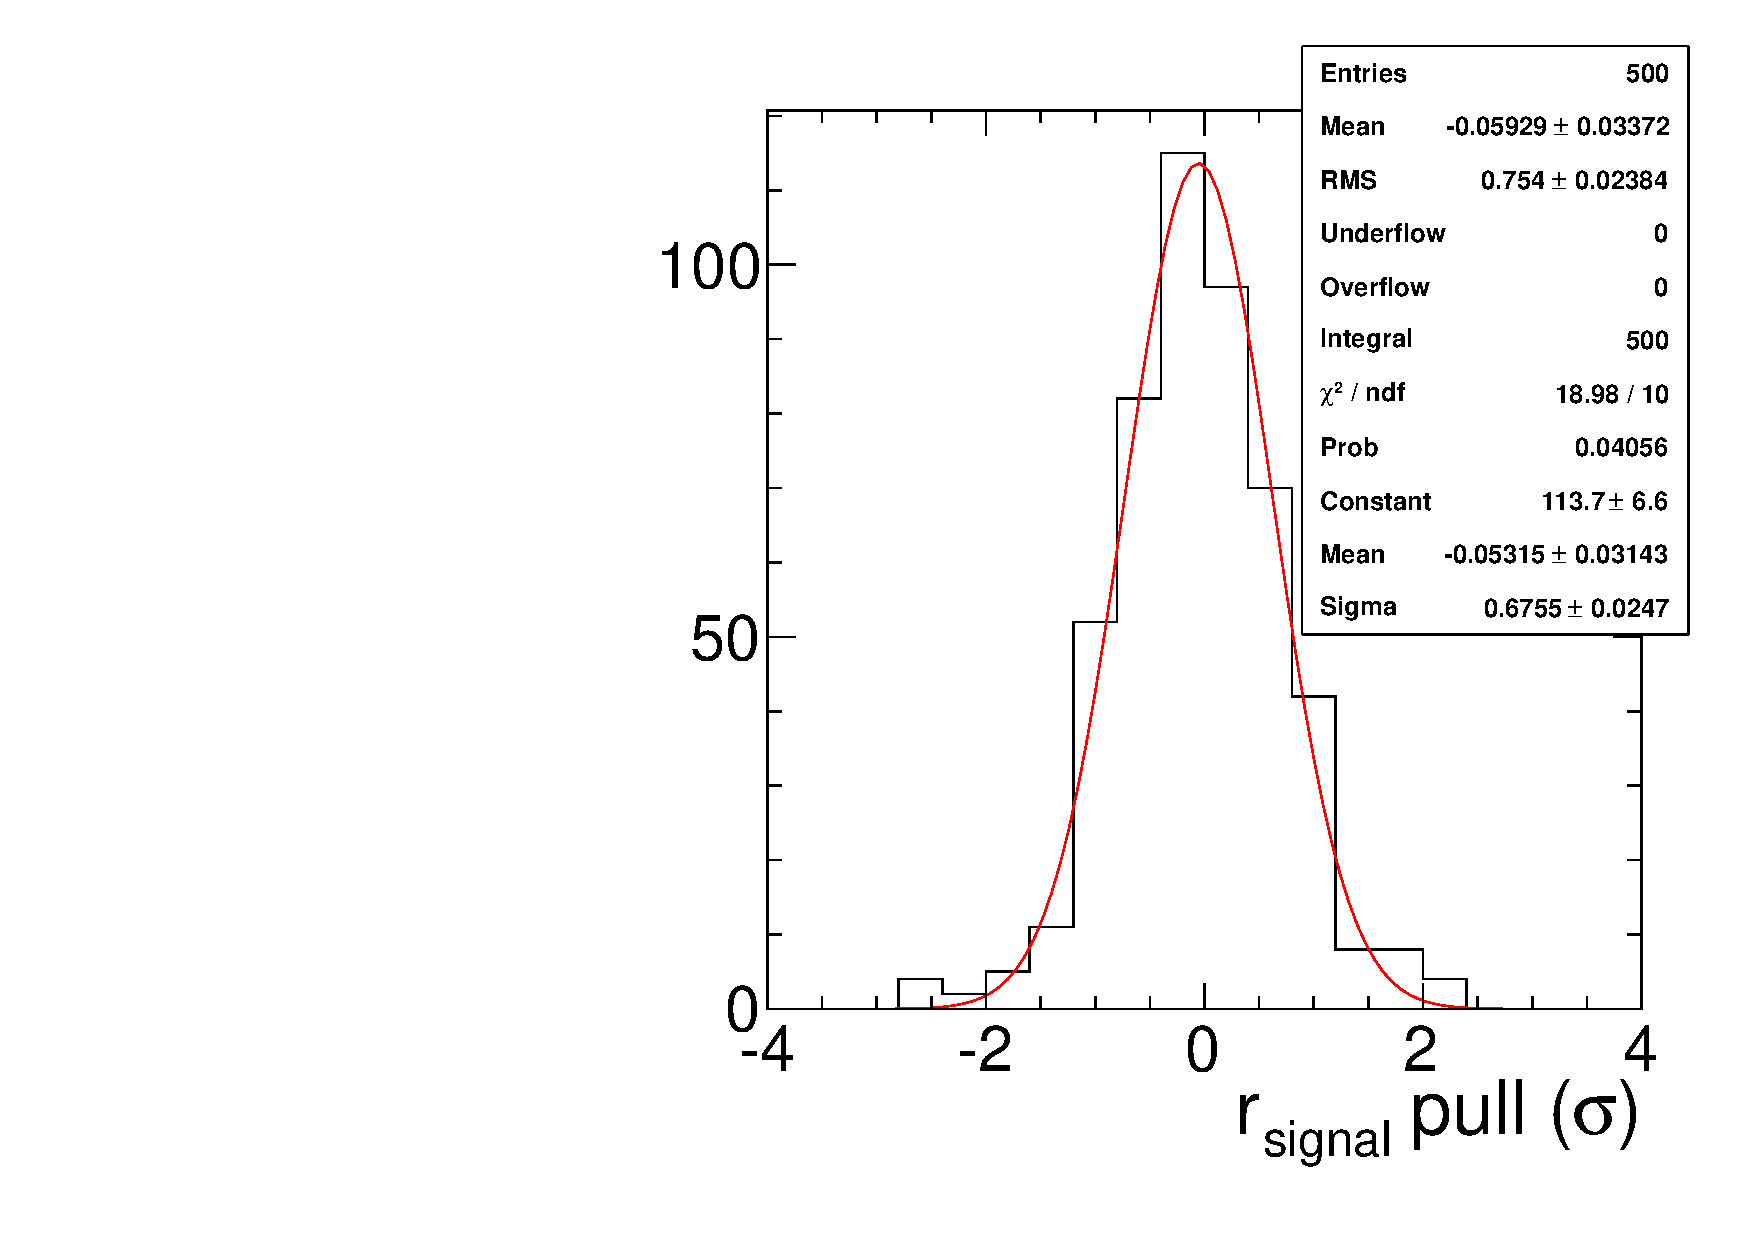
\includegraphics[width=0.4\textwidth]{plots/ML_validation/HWW200_Sig0_0_ToyResults_pull}
  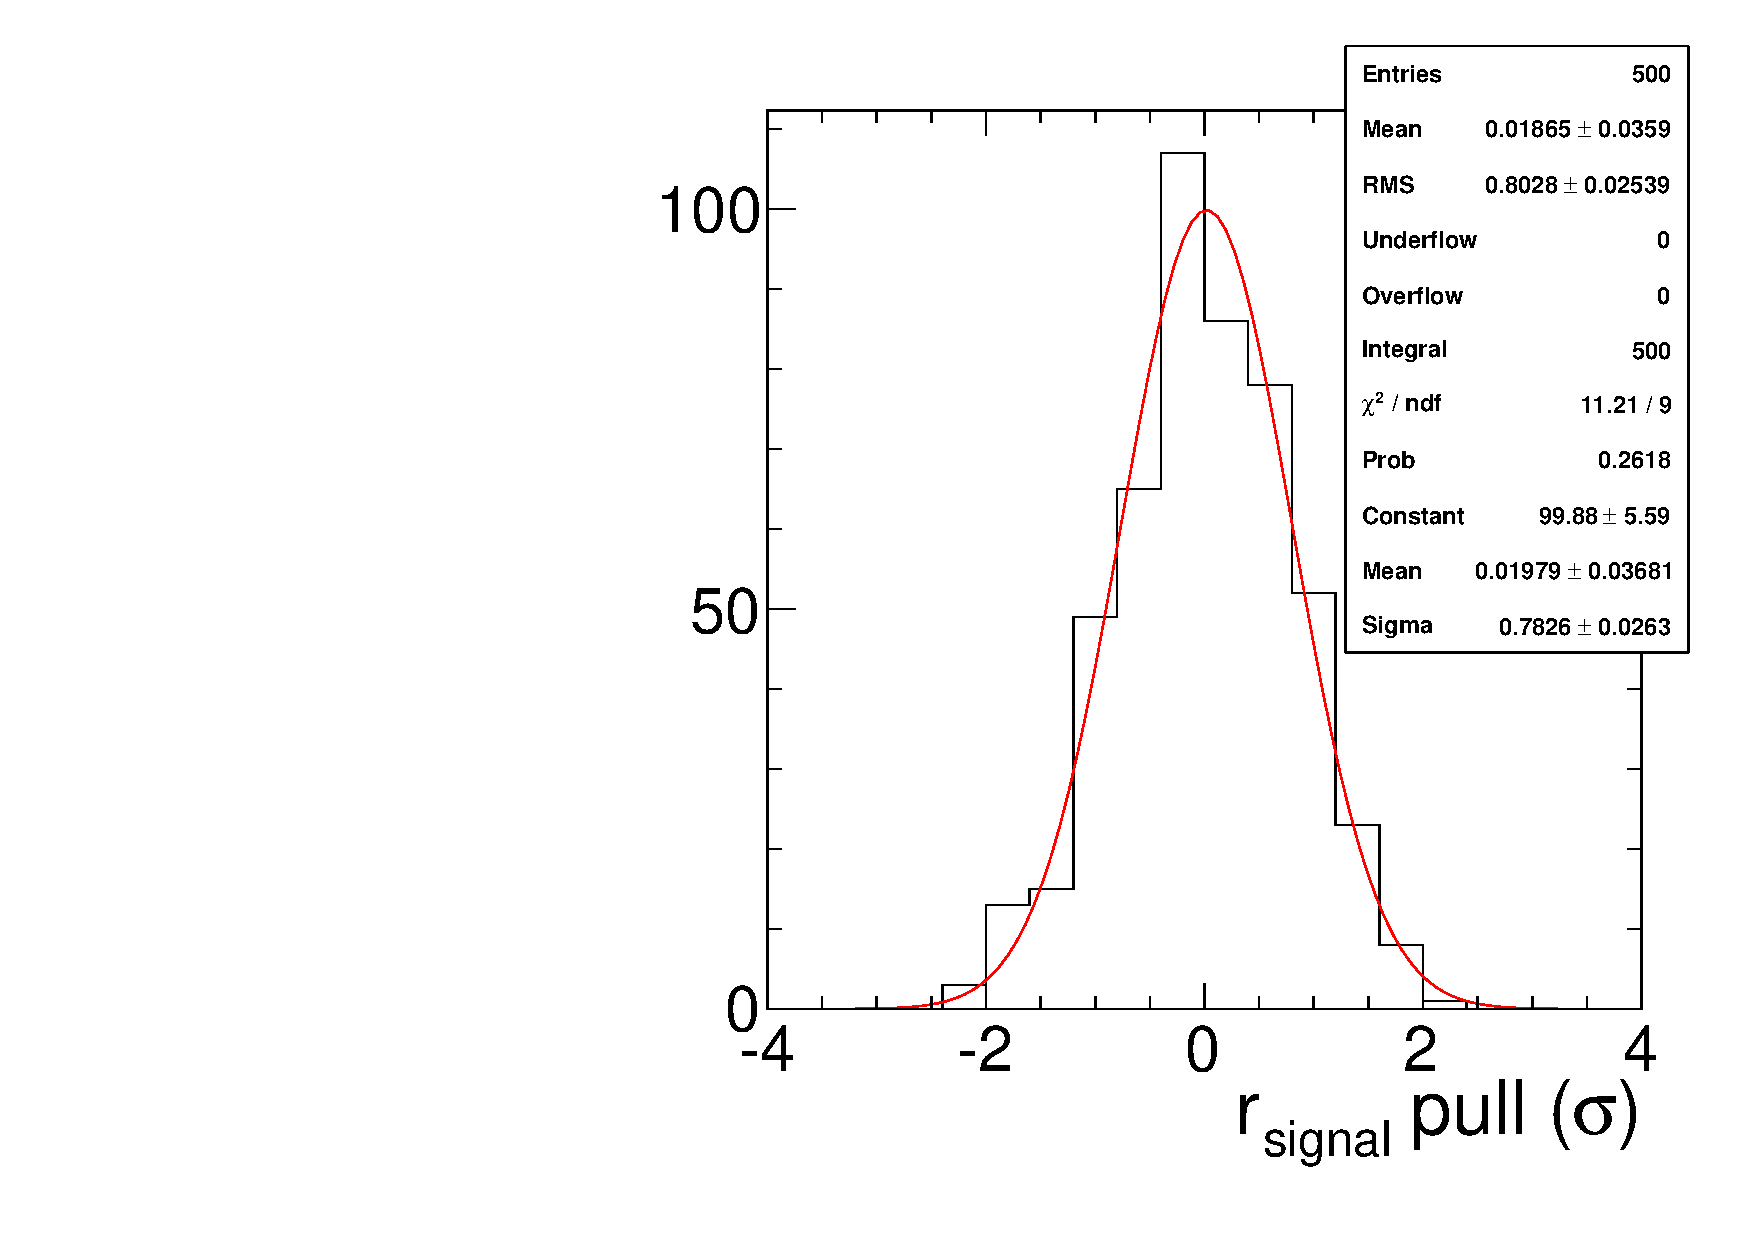
\includegraphics[width=0.4\textwidth]{plots/ML_validation/HWW300_Sig0_0_ToyResults_pull}
  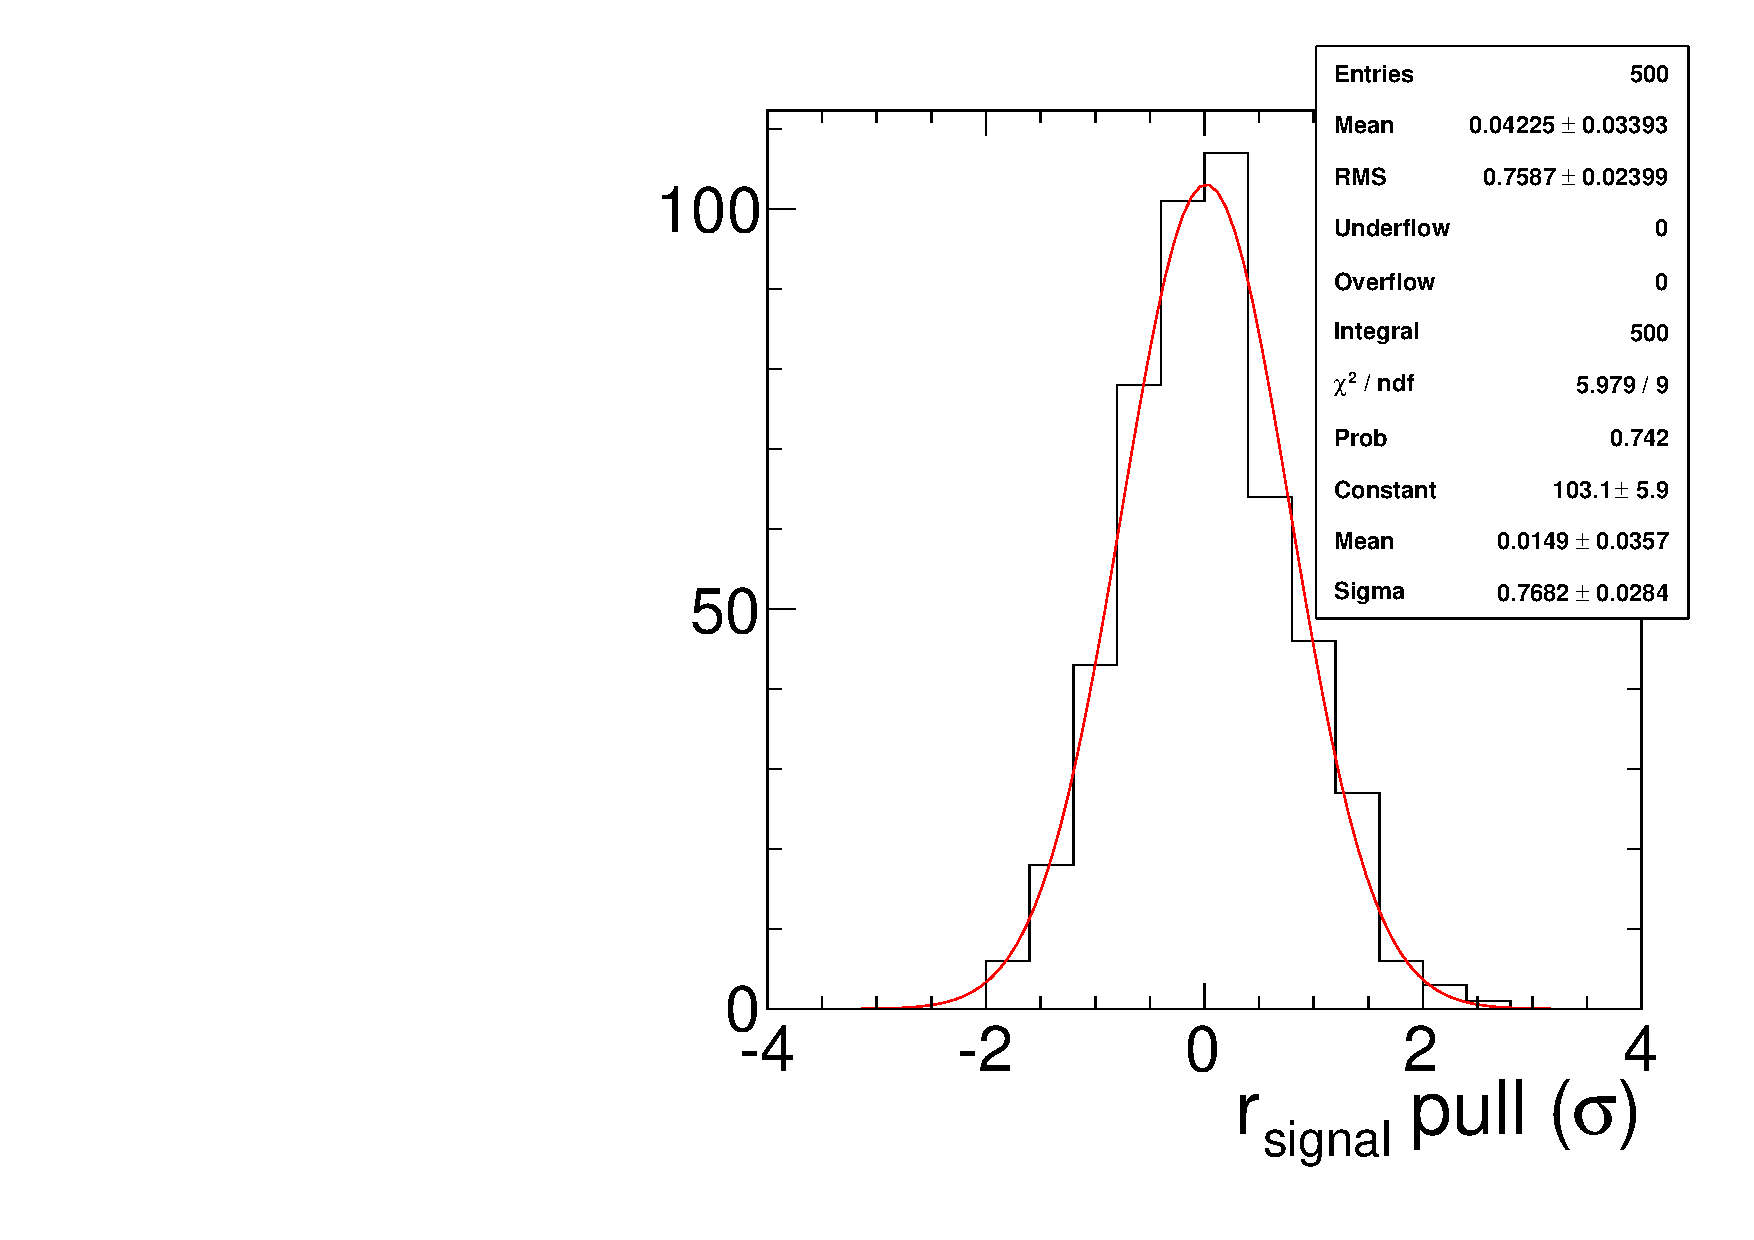
\includegraphics[width=0.4\textwidth]{plots/ML_validation/HWW400_Sig0_0_ToyResults_pull}
  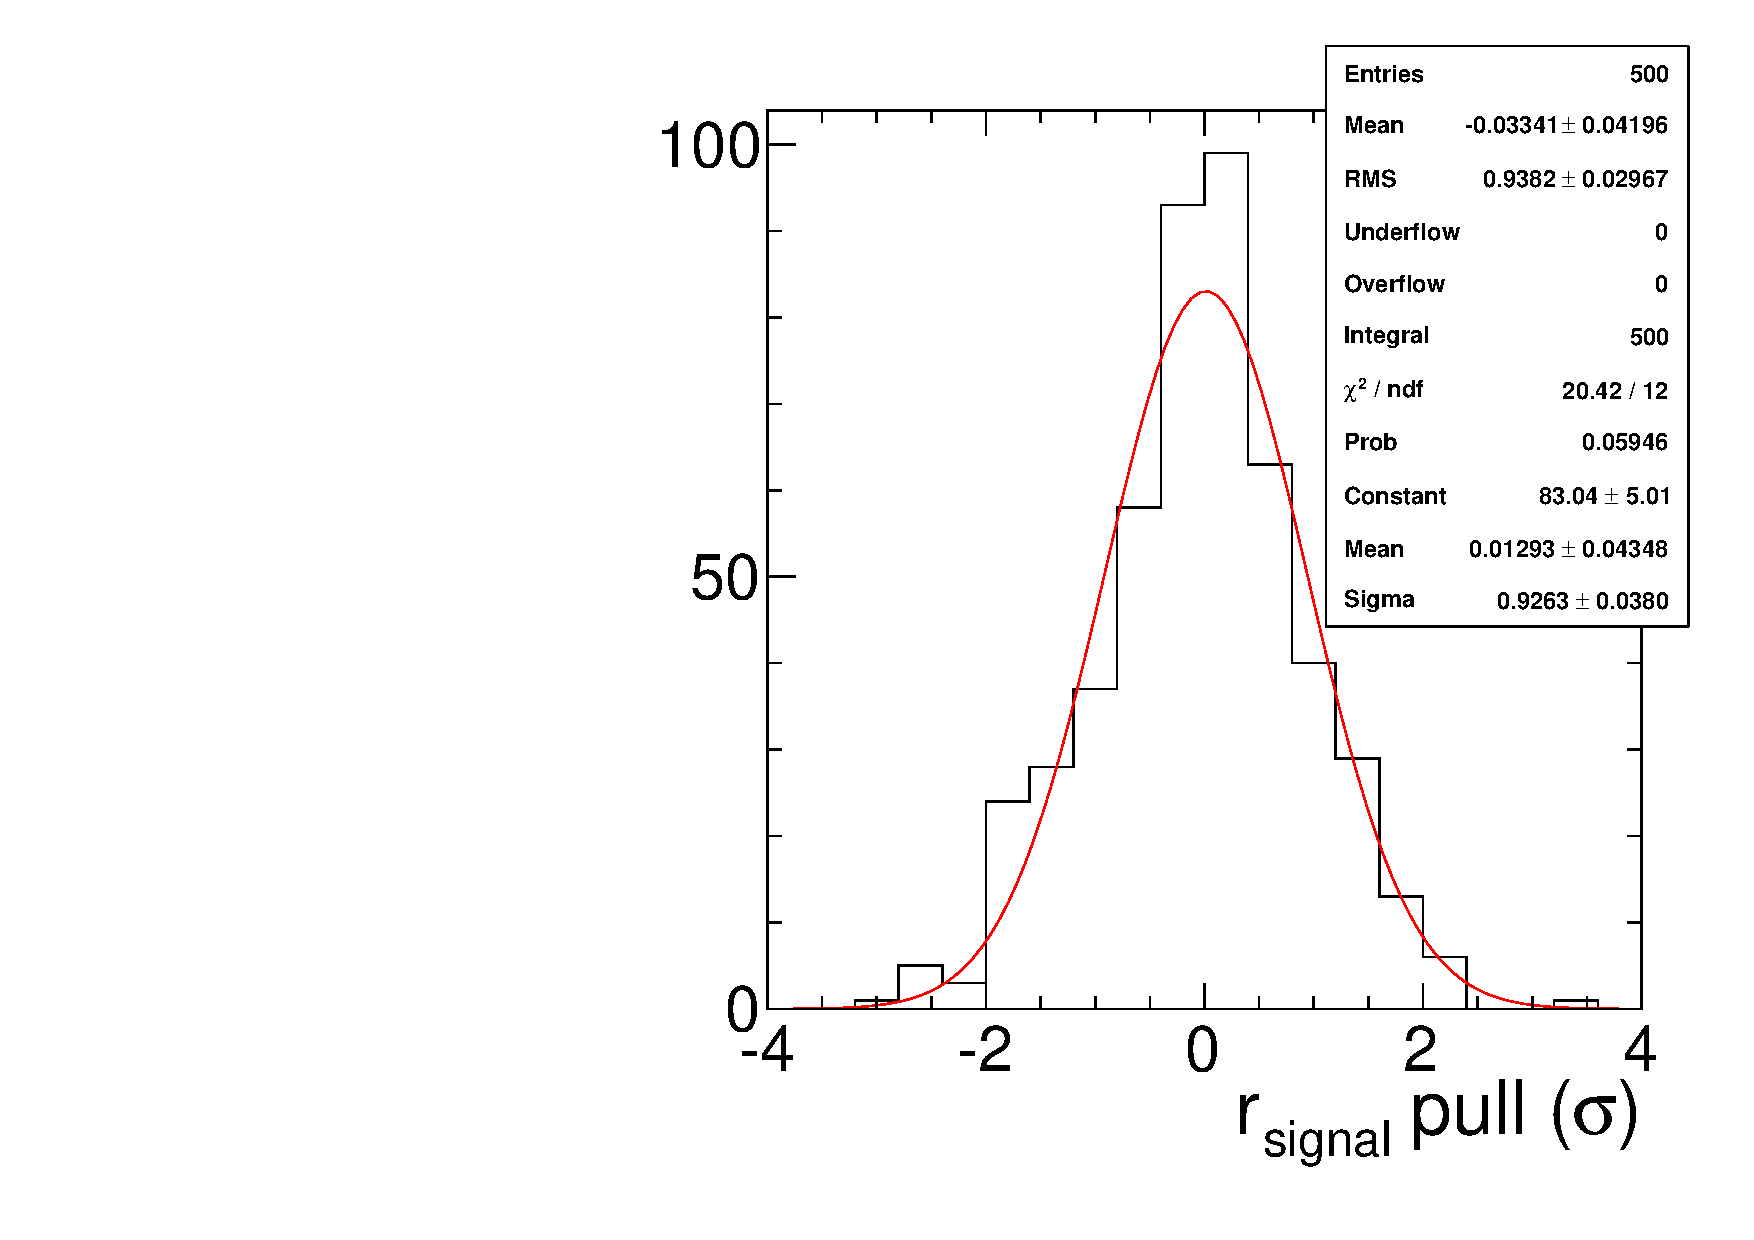
\includegraphics[width=0.4\textwidth]{plots/ML_validation/HWW600_Sig0_0_ToyResults_pull}
\end{center}
\caption{\label{fig:validation0}Pull ($(r_\text{fit}-r_\text{gen})/\sigma_{r}$)
for the mass points beginning at the upper left 180, 200, 300, 400, 600, under the zero signal generation.}
\end{figure}

\begin{figure}
\begin{center}
  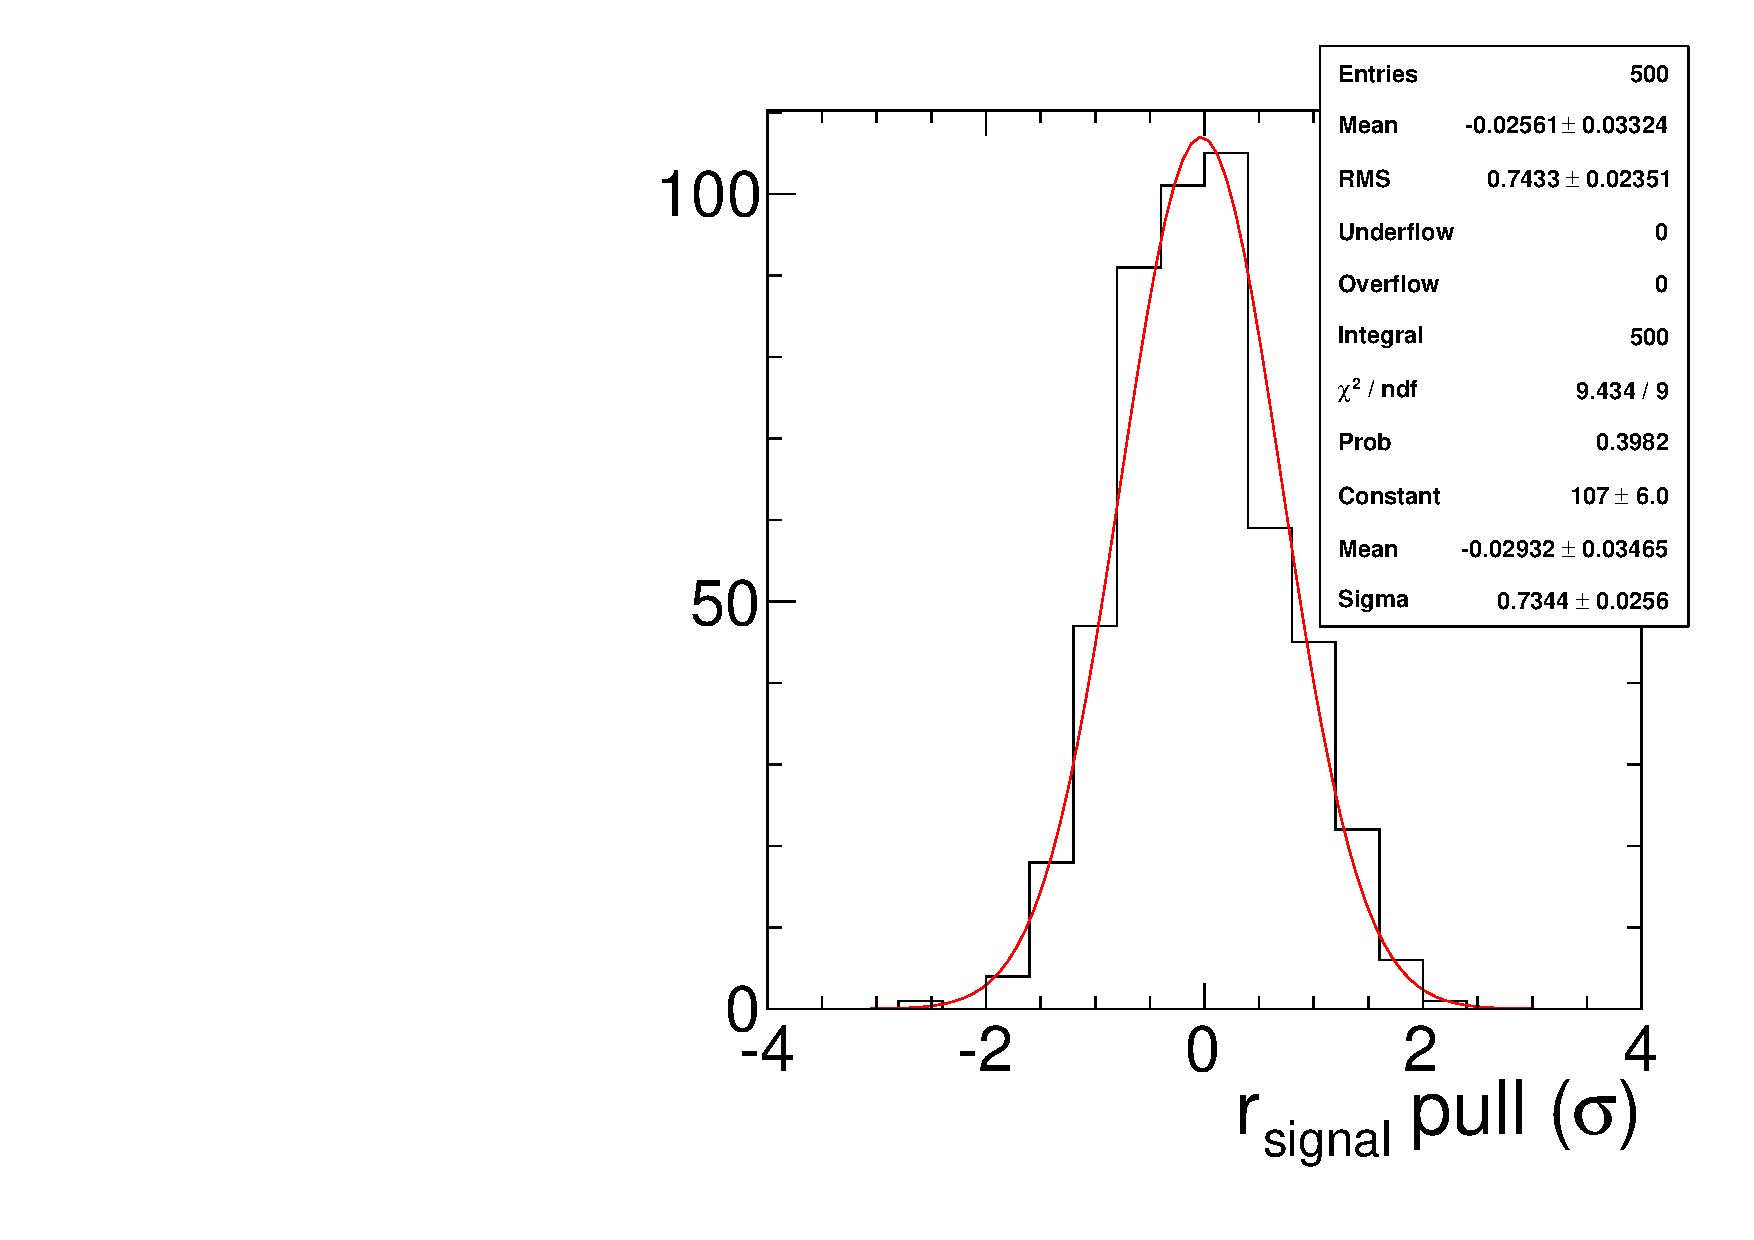
\includegraphics[width=0.4\textwidth]{plots/ML_validation/HWW180_Sig1_0_ToyResults_pull}
  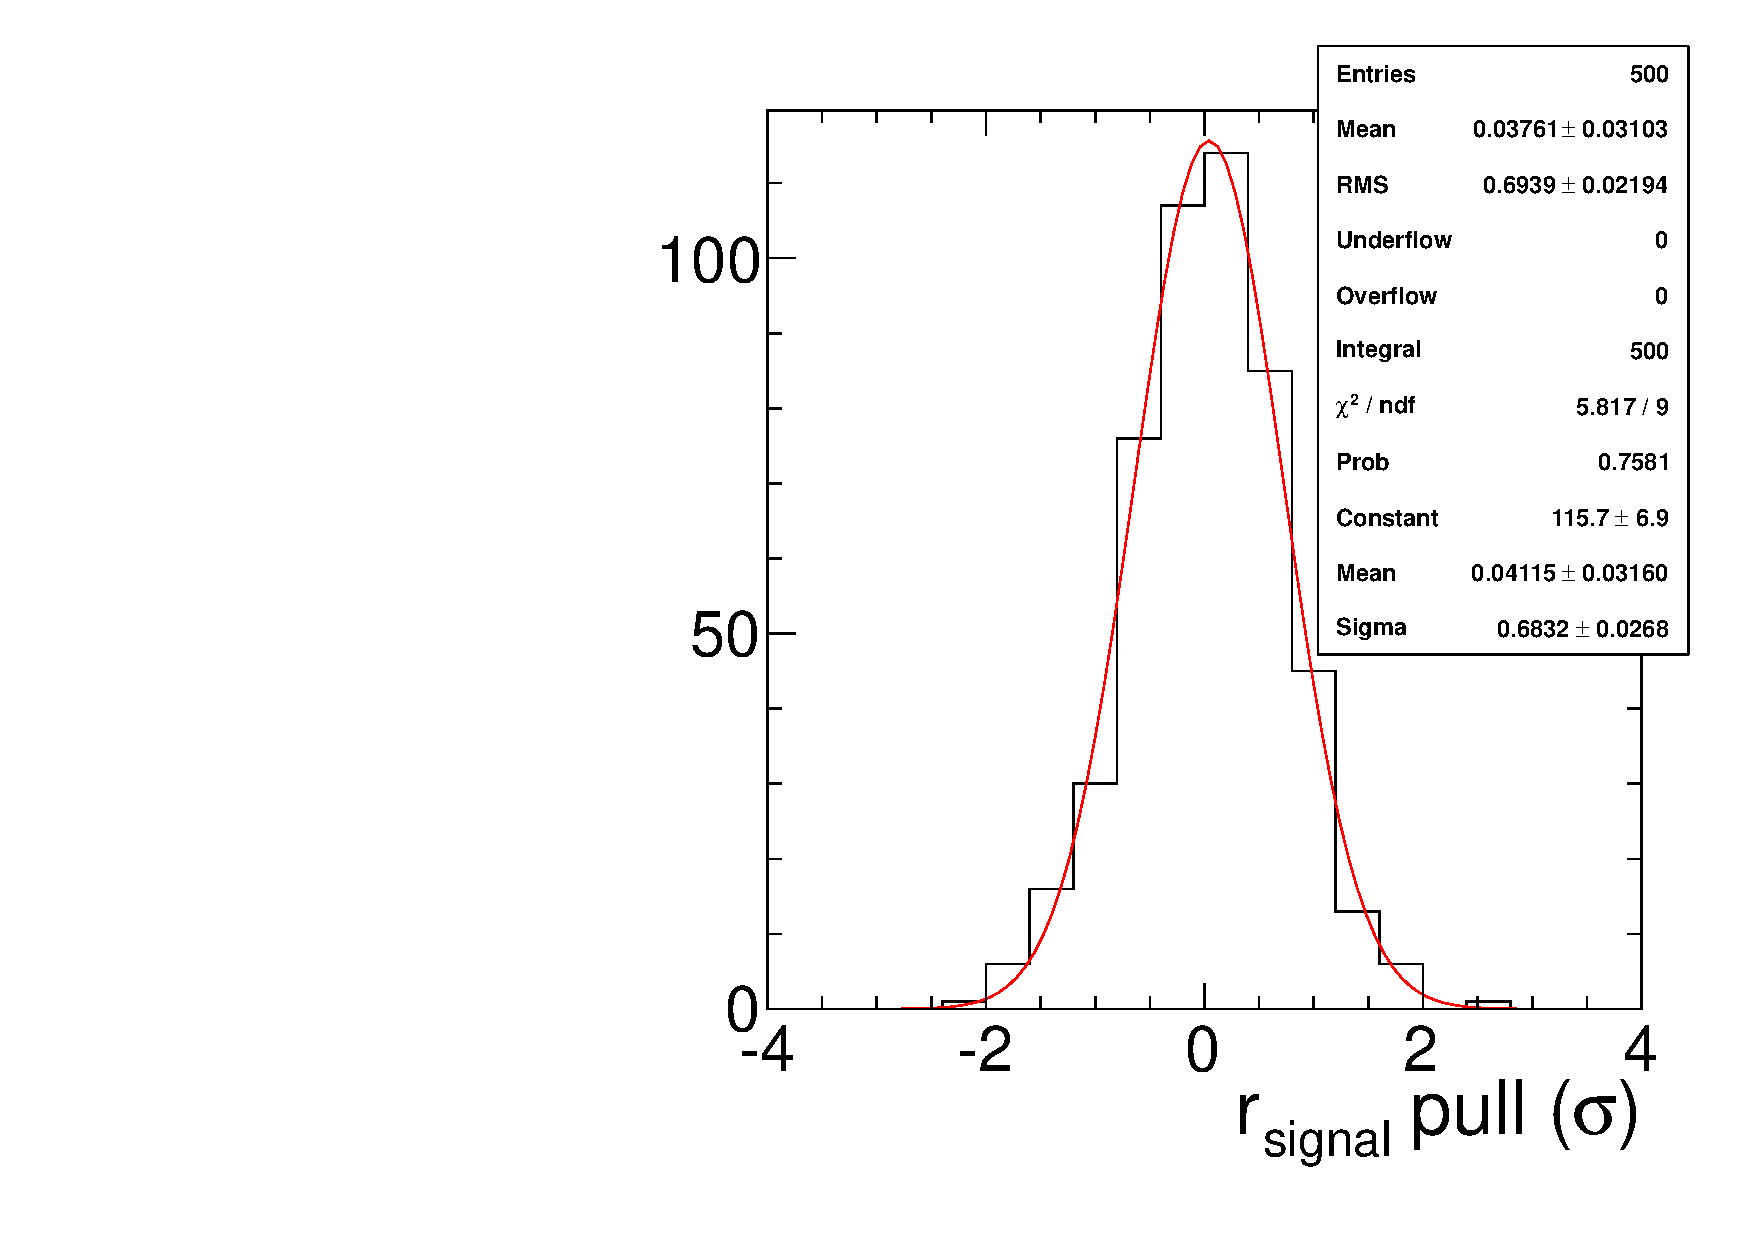
\includegraphics[width=0.4\textwidth]{plots/ML_validation/HWW200_Sig1_0_ToyResults_pull}
  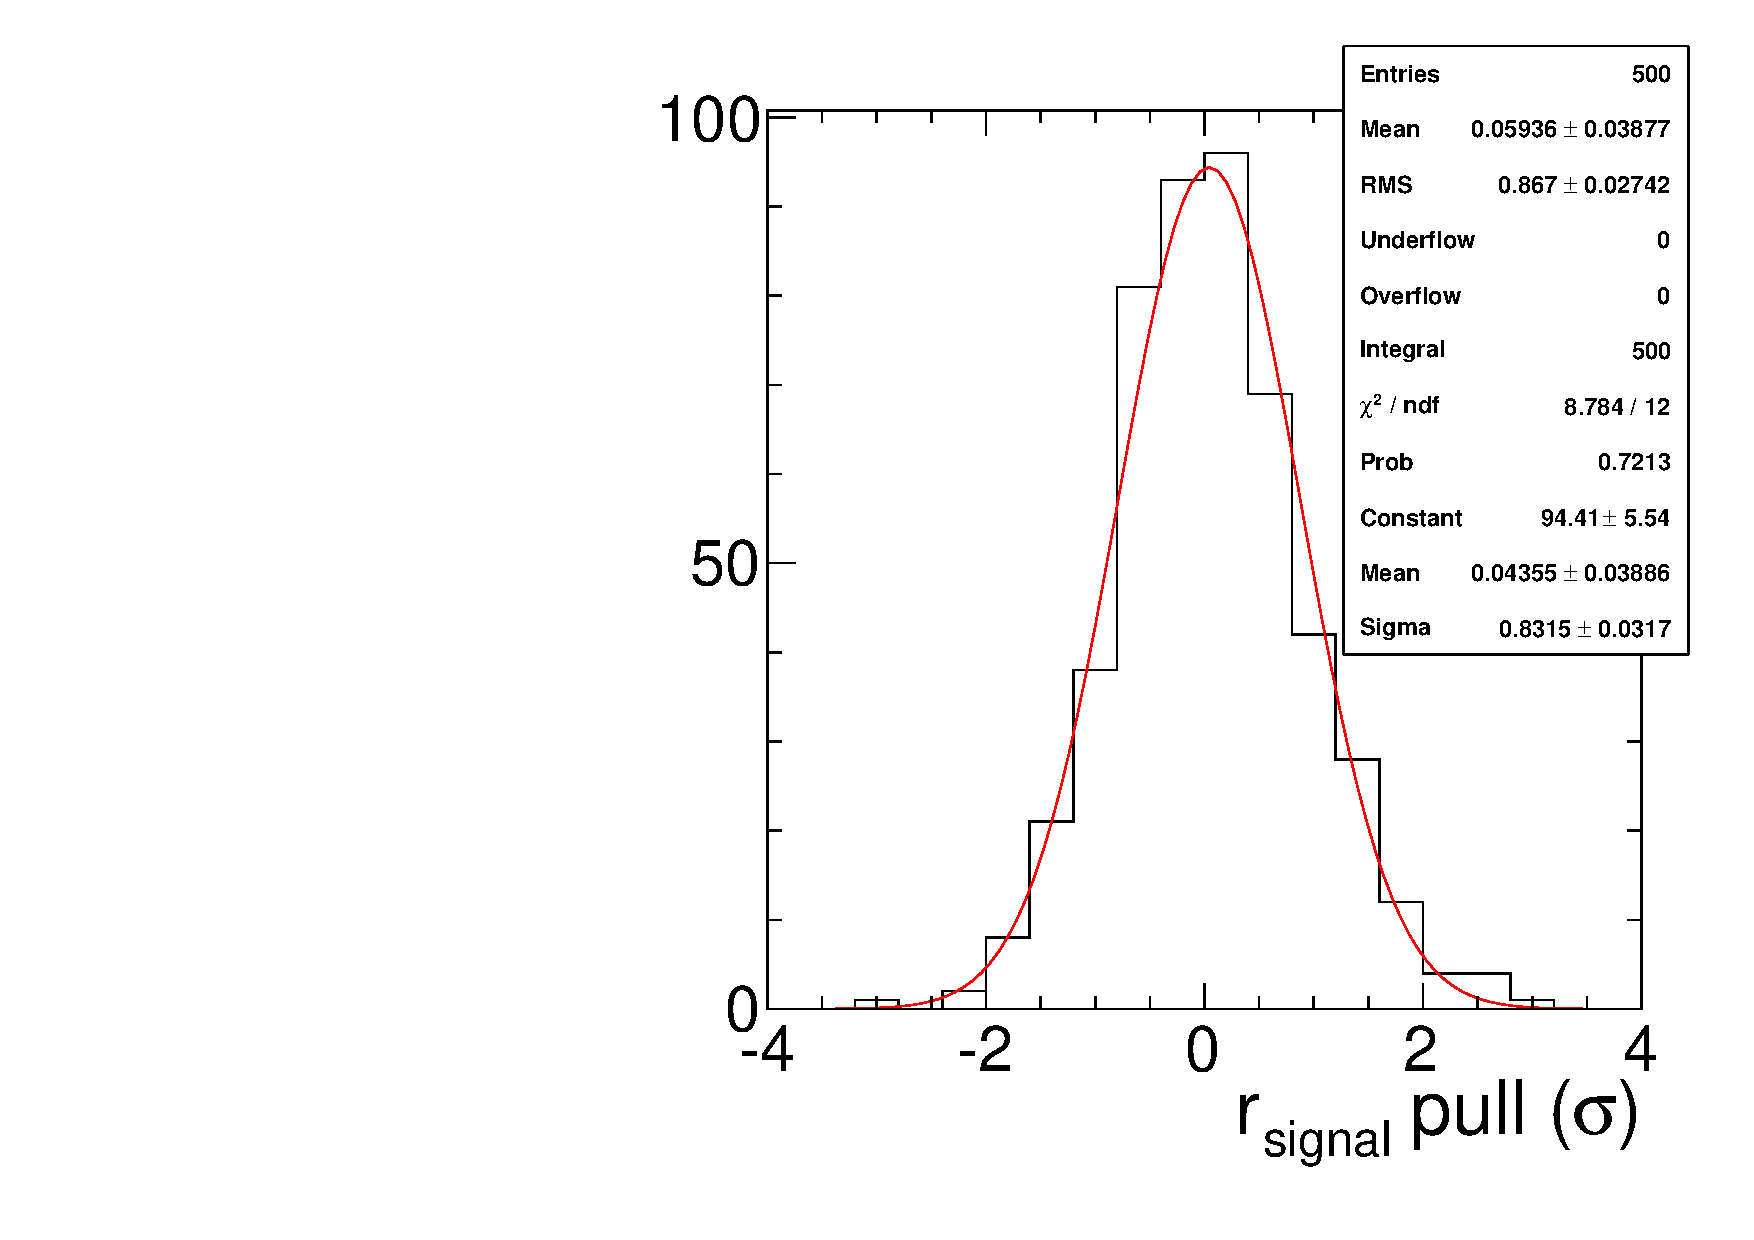
\includegraphics[width=0.4\textwidth]{plots/ML_validation/HWW300_Sig1_0_ToyResults_pull}
  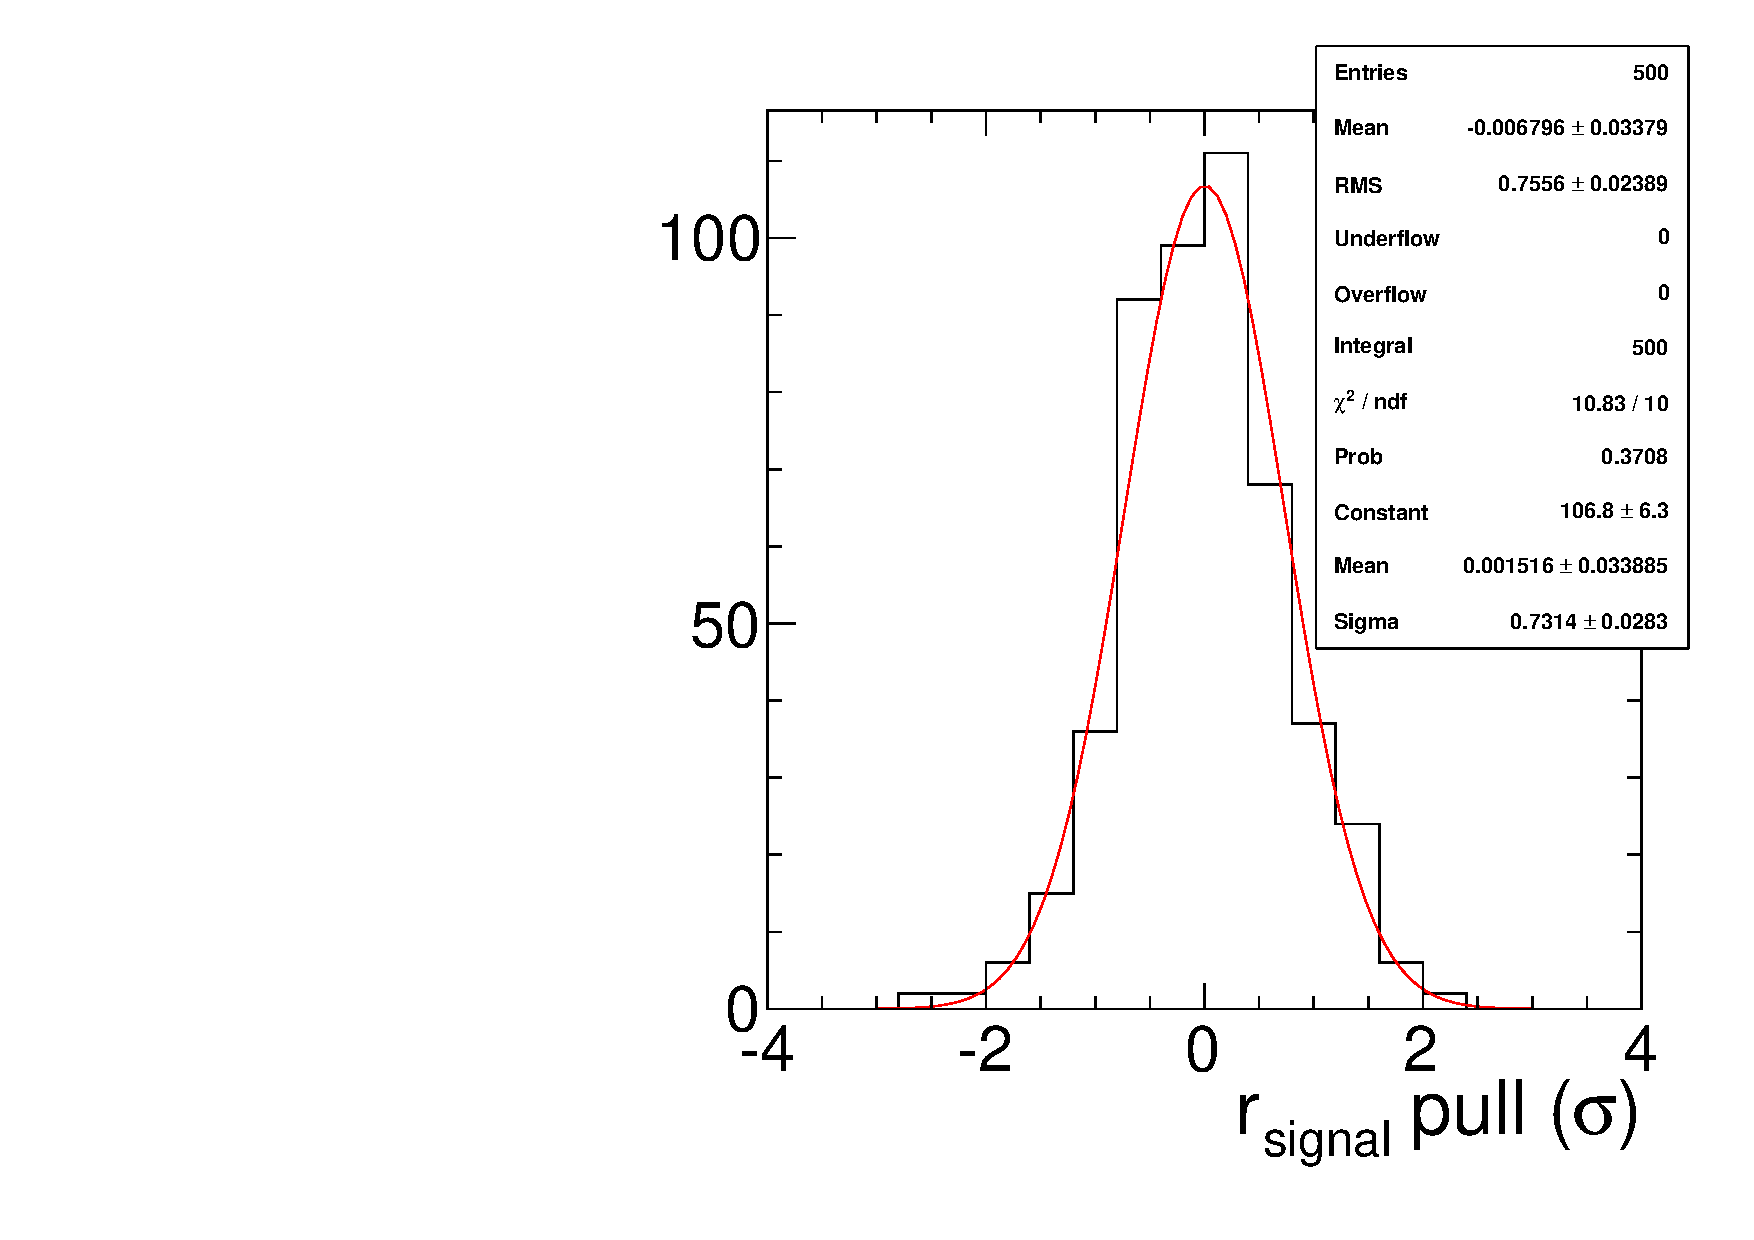
\includegraphics[width=0.4\textwidth]{plots/ML_validation/HWW400_Sig1_0_ToyResults_pull}
  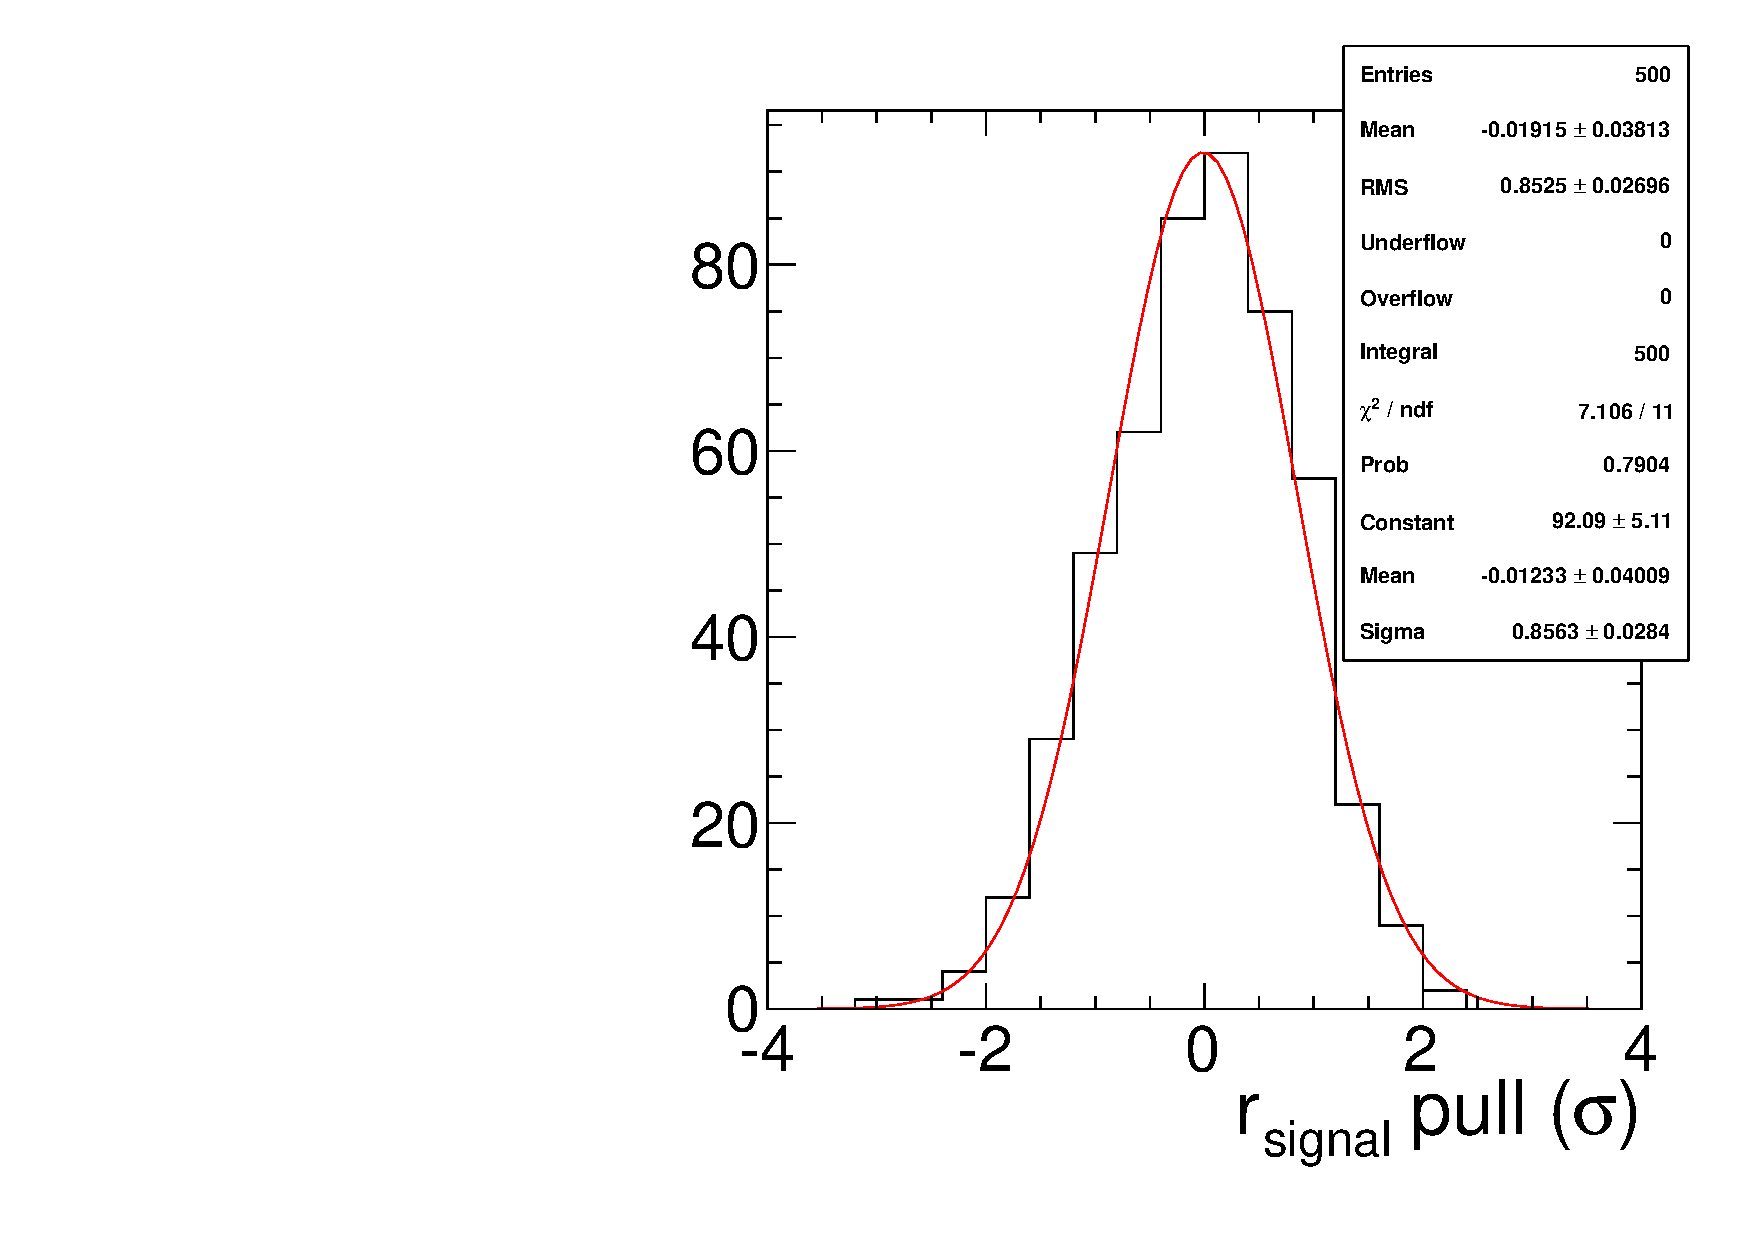
\includegraphics[width=0.4\textwidth]{plots/ML_validation/HWW600_Sig1_0_ToyResults_pull}
\end{center}
\caption{\label{fig:validation1}Pull ($(r_\text{fit}-r_\text{gen})/\sigma_{r}$)
for the mass points beginning at the upper left 180, 200, 300, 400, 600, under the $1\times$ signal generation.}
\end{figure}

\begin{figure}
\begin{center}
  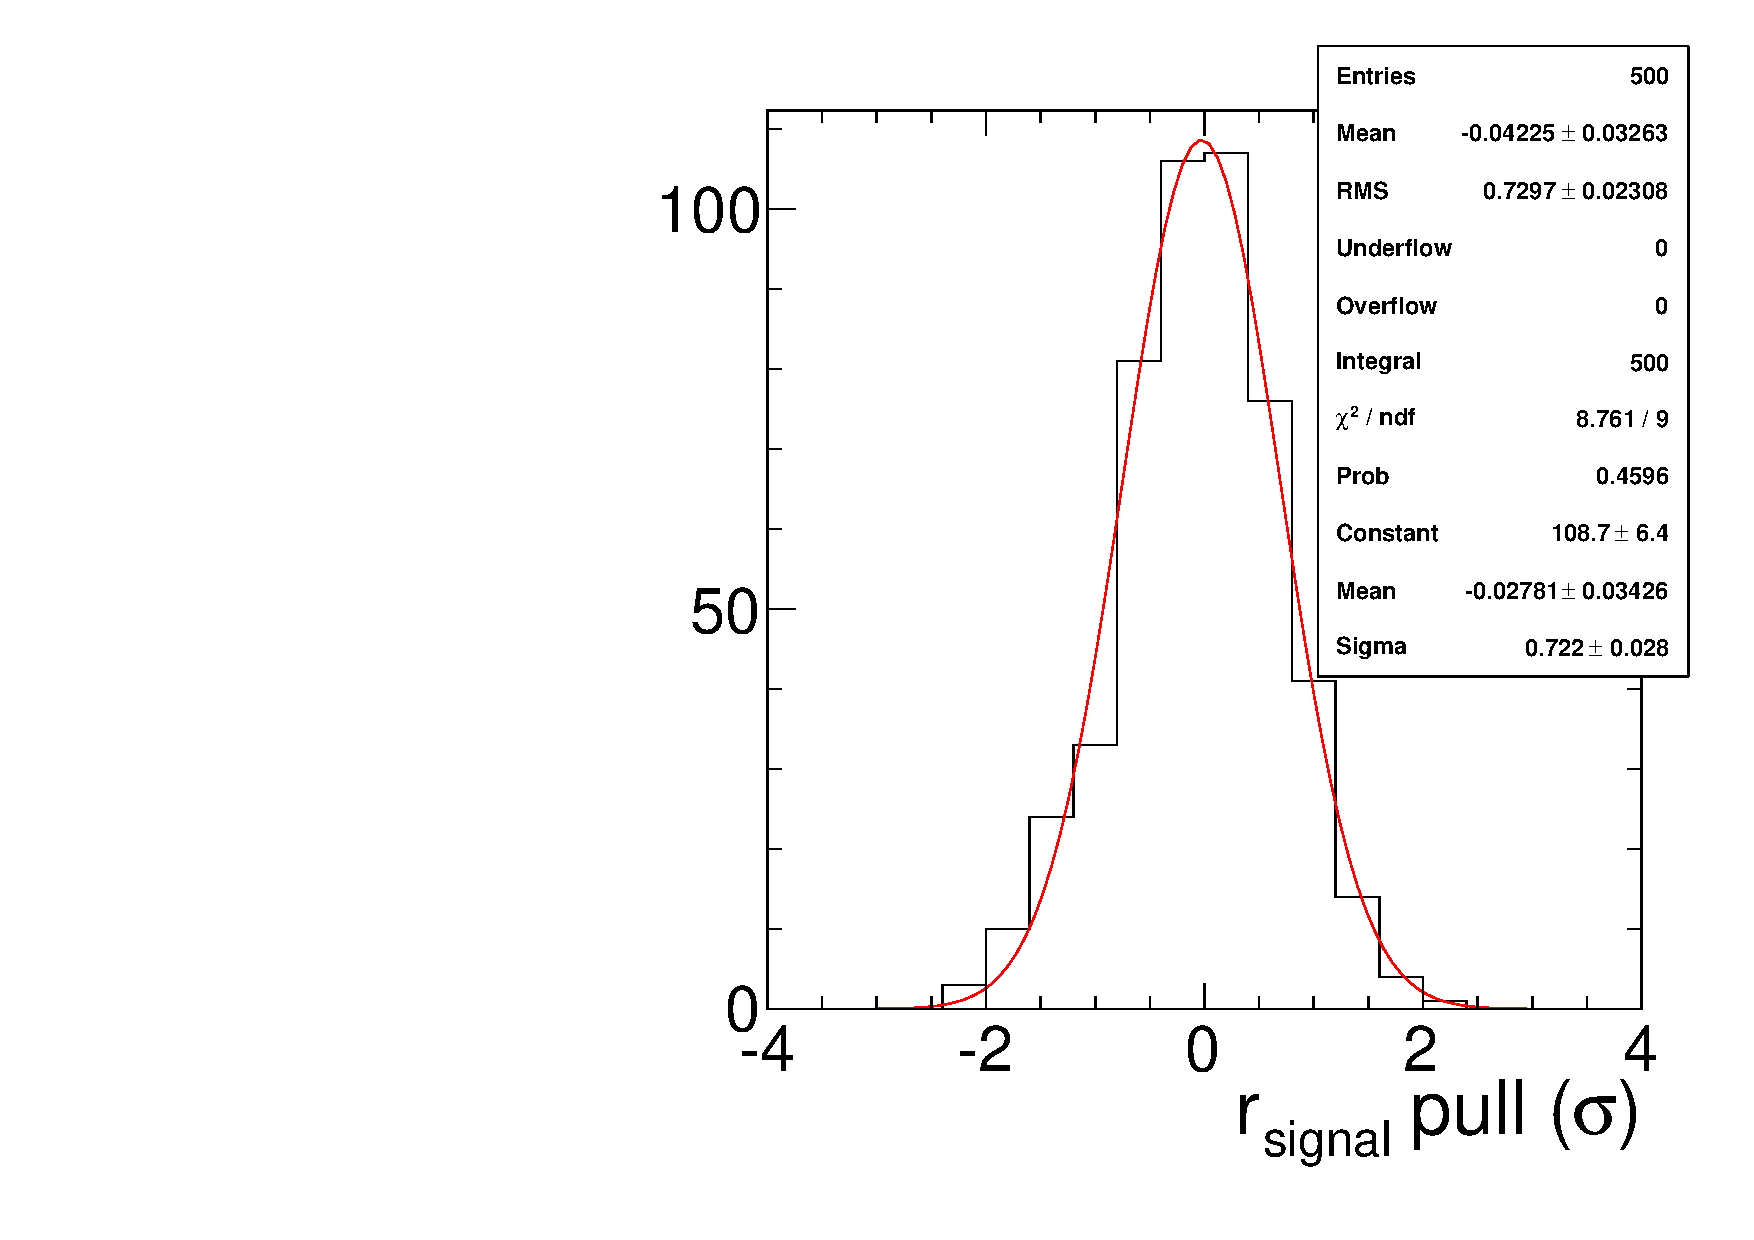
\includegraphics[width=0.4\textwidth]{plots/ML_validation/HWW180_Sig2_0_ToyResults_pull}
  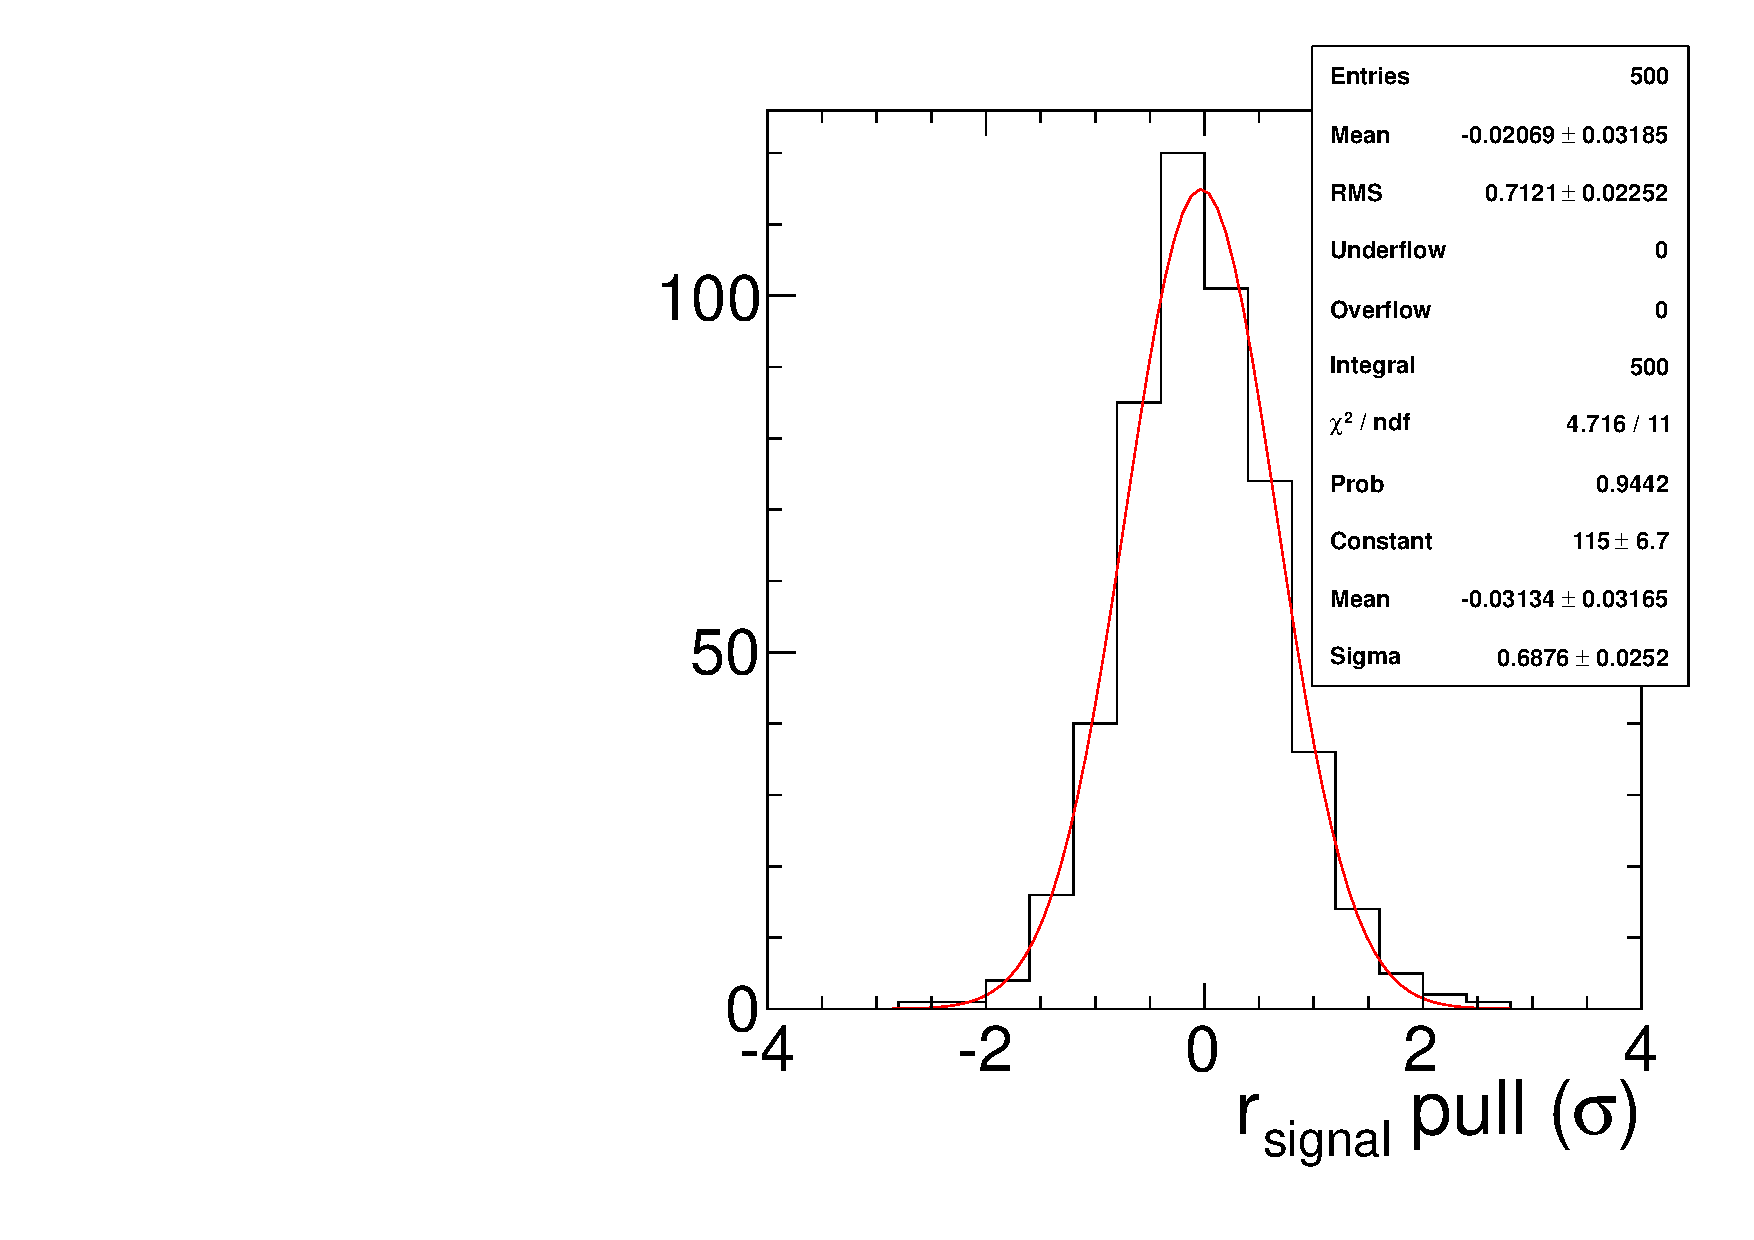
\includegraphics[width=0.4\textwidth]{plots/ML_validation/HWW200_Sig2_0_ToyResults_pull}
  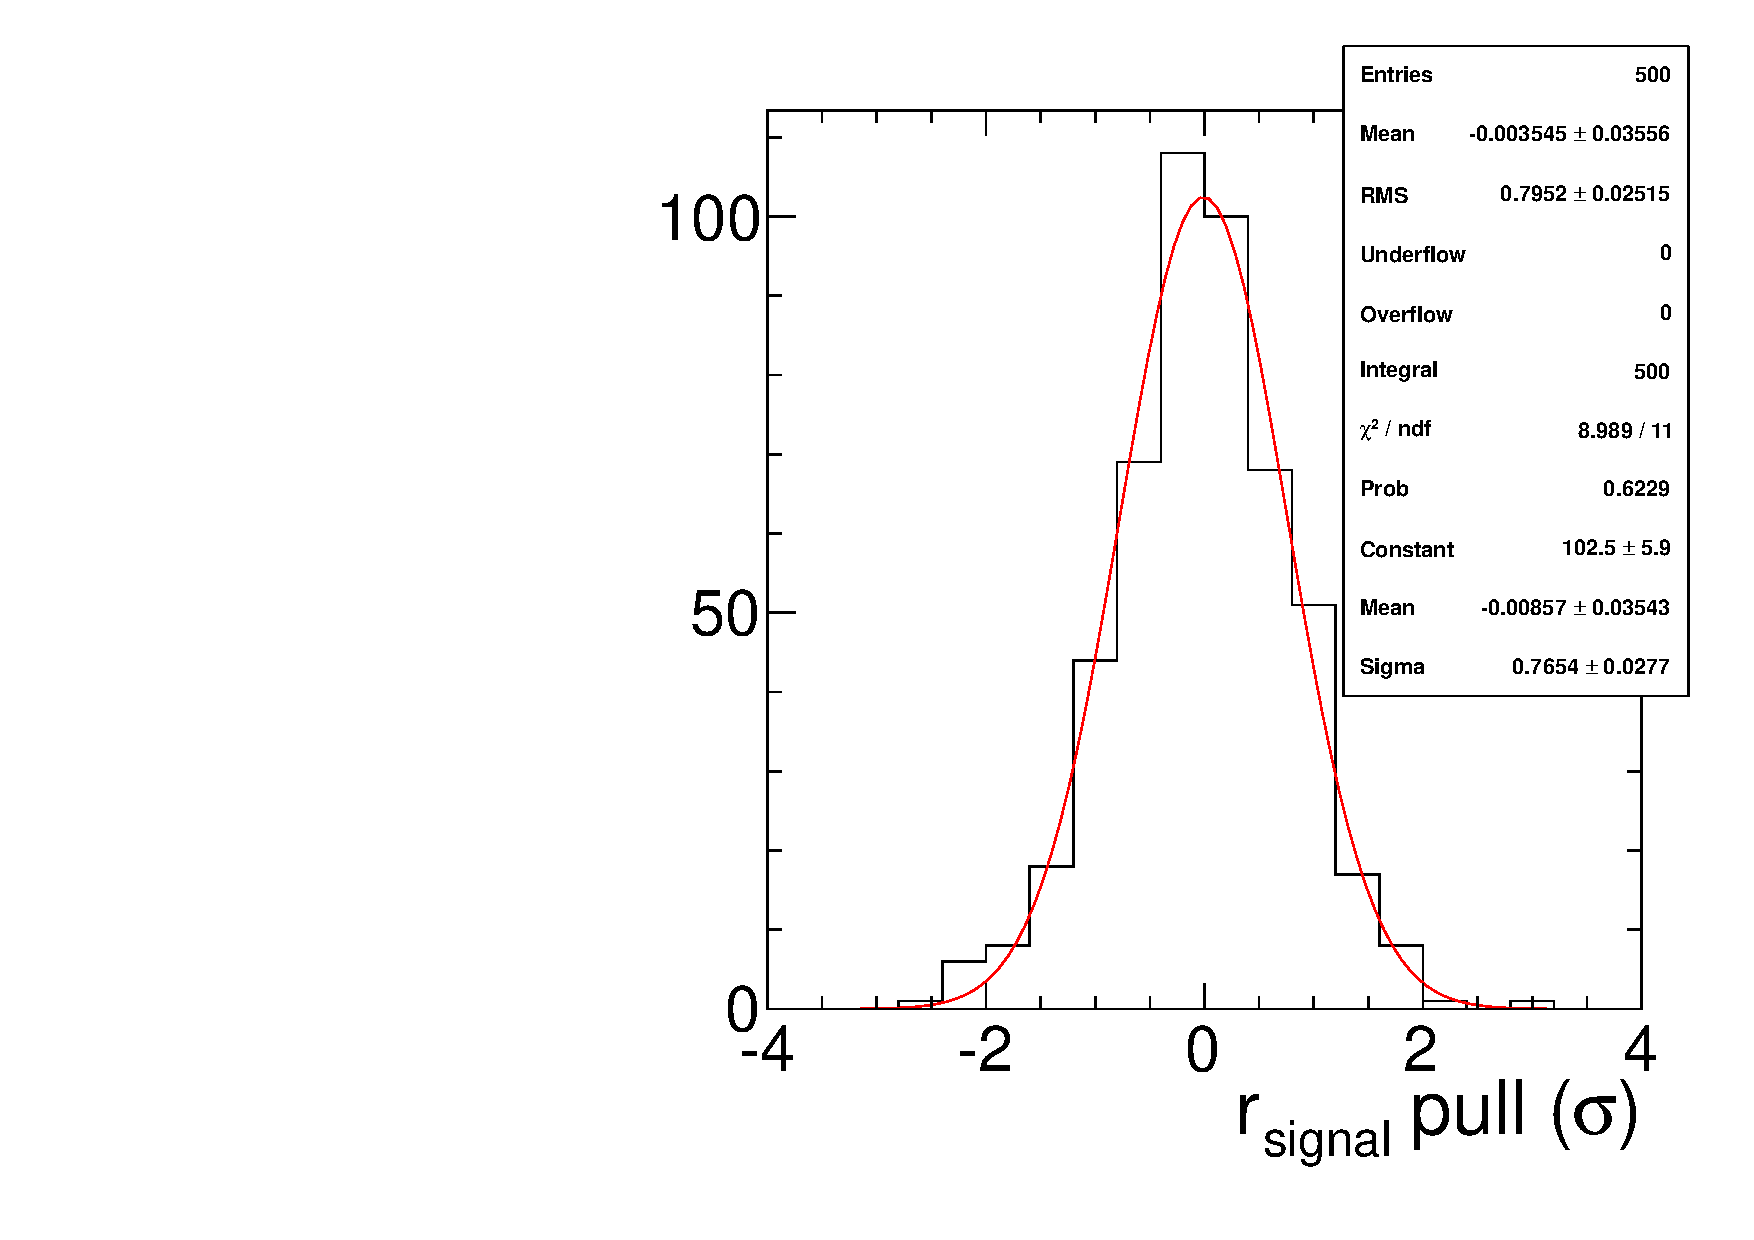
\includegraphics[width=0.4\textwidth]{plots/ML_validation/HWW300_Sig2_0_ToyResults_pull}
  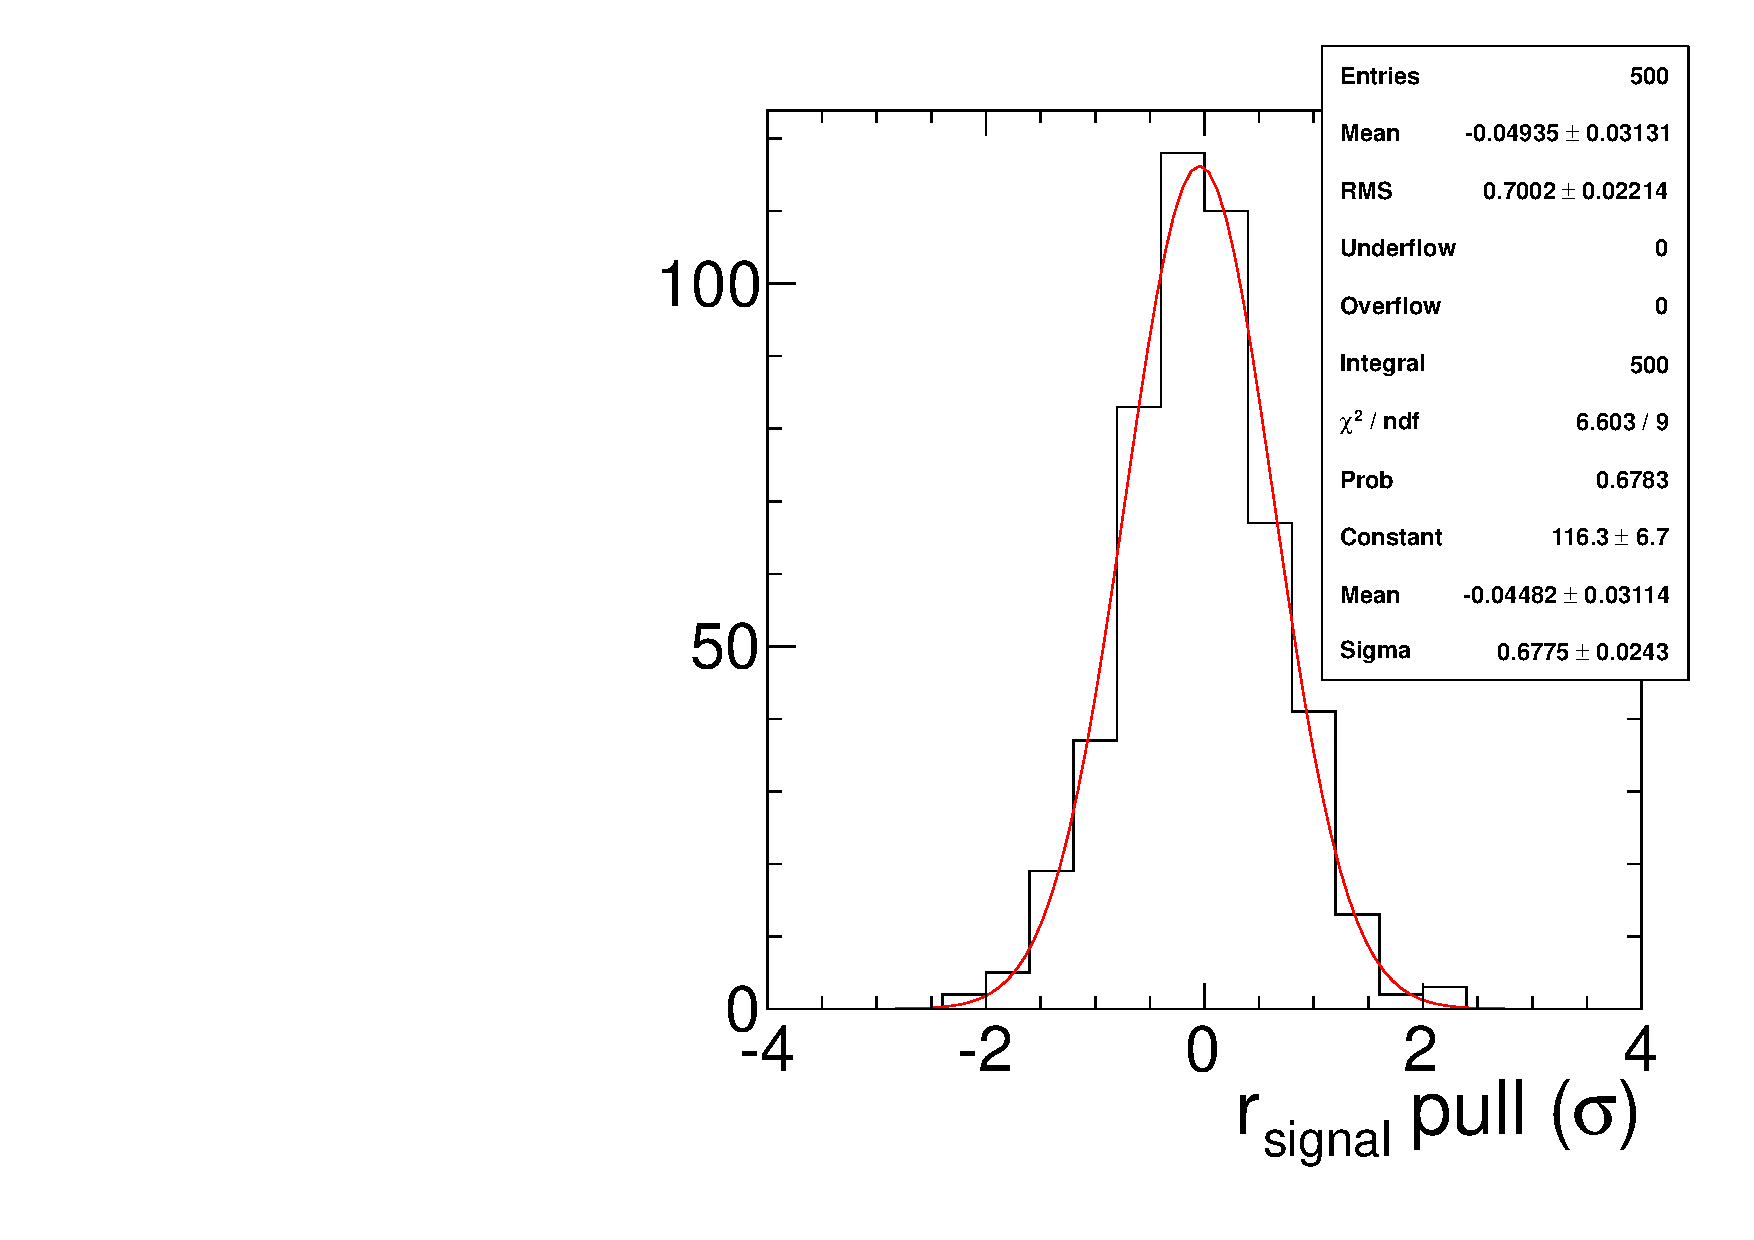
\includegraphics[width=0.4\textwidth]{plots/ML_validation/HWW400_Sig2_0_ToyResults_pull}
  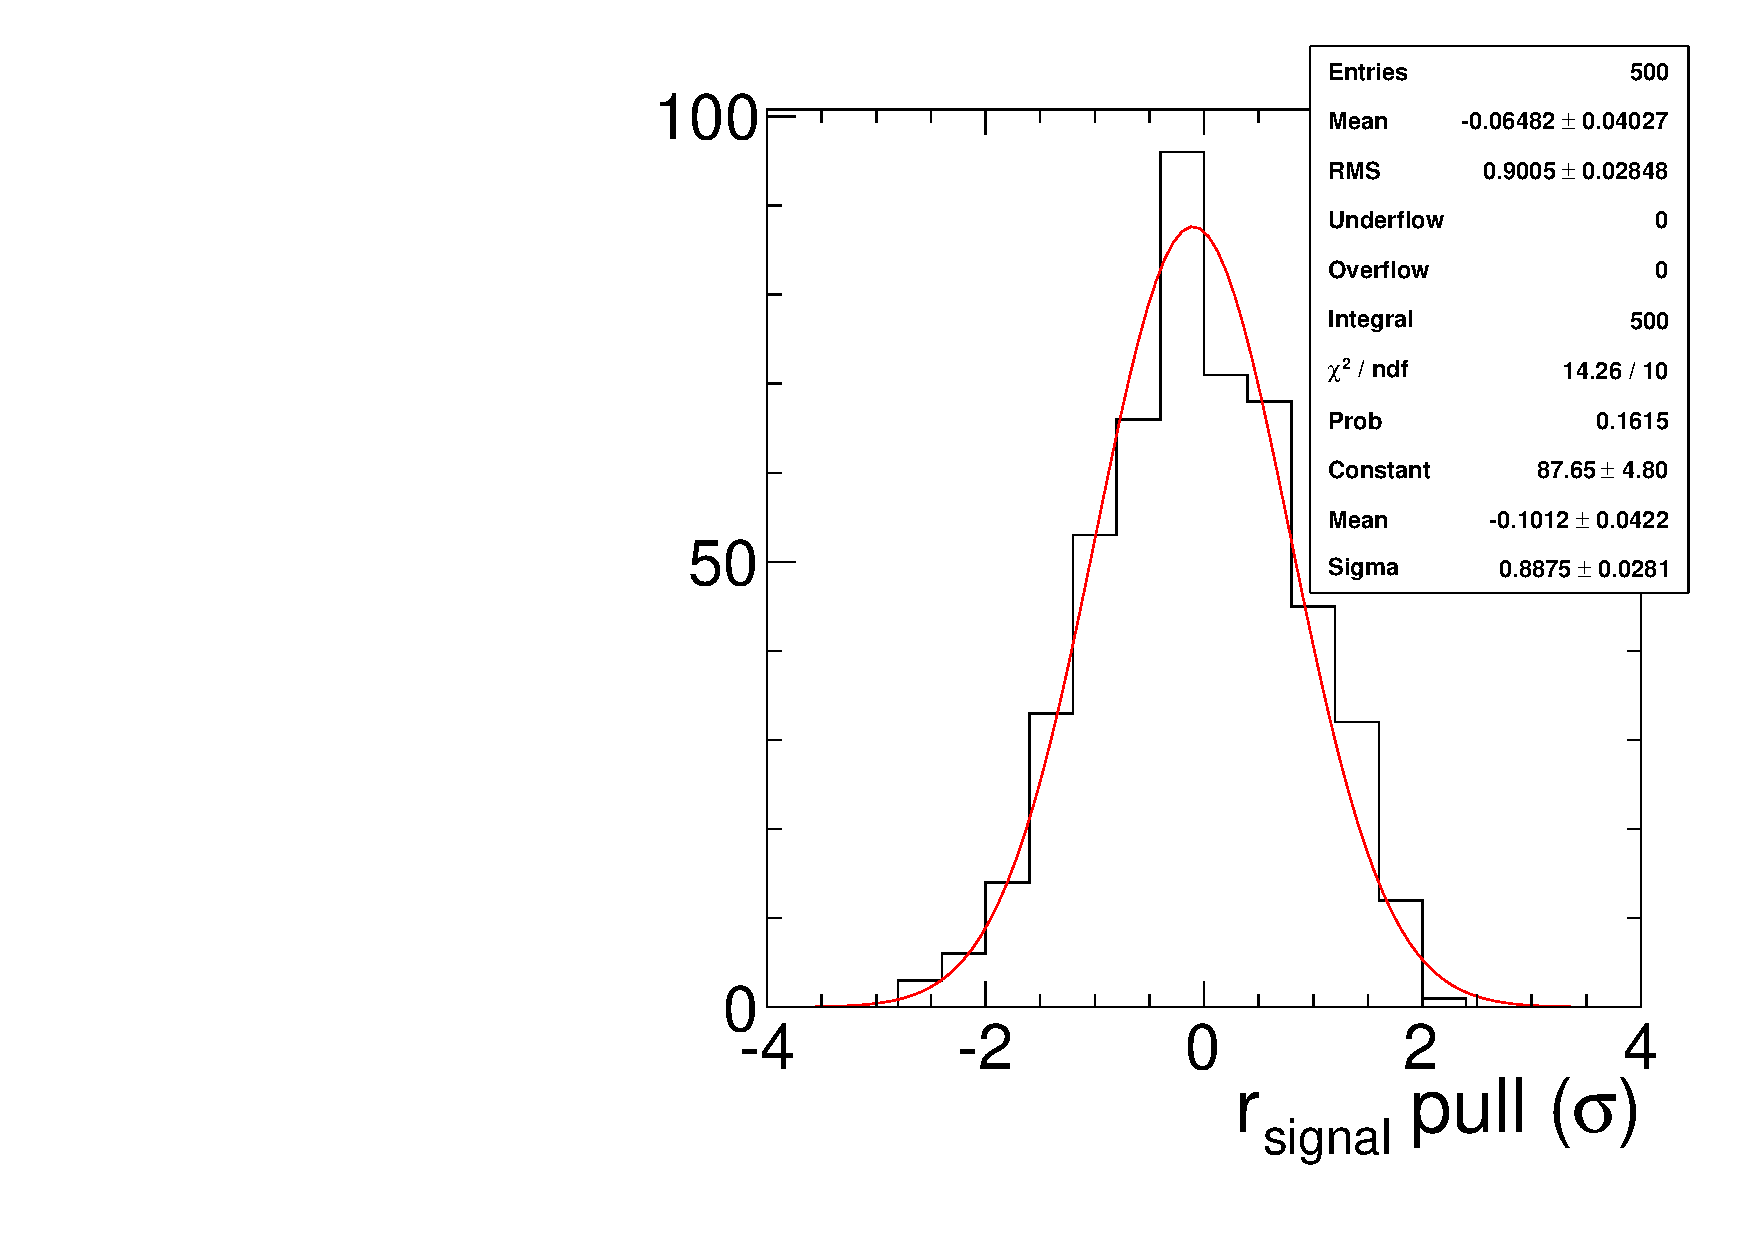
\includegraphics[width=0.4\textwidth]{plots/ML_validation/HWW600_Sig2_0_ToyResults_pull}
\end{center}
\caption{\label{fig:validation2}Pull ($(r_\text{fit}-r_\text{gen})/\sigma_{r}$)
for the mass points beginning at the upper left 180, 200, 300, 400, 600, under the $2\times$ signal generation.}
\end{figure}

\subsection{Determination of the normalization from fits to dijet mass}
\label{sec:mjjfitfornormal}
% .... .... .... .... .... .... .... .... .... .... .... .... .... .... .... .... .... .... .... .... .... .... ....

We extract the background yields from an unbinned maximum likelihood
fit to the dijet invariant mass distribution $m_{jj}$, after the selection on the MVA discriminant,
excluding the signal region ($66~{\mbox{GeV}} < m_{jj} < 98~{\mbox{GeV}}$). 
% Events in the signal region are later used to set Higgs exclusion limits. 
In this fit, all the backgrounds are considered. 
The W+jets shape is as described in Section~\ref{sec:wjetsShape},
% the QCD shape as described in Section~\ref{sec:dataDrivenQCD}, 
while the other background shapes come from the simulation.  The dijet
mass spectrum fit provides inputs for the yields of the physics
processes.  Table~\ref{tab:mjj_shapes_and_normalization} shows in a
schematic view how the shape of each component is determined, and what
constraints are applied to fit for the normalization.

\begin{table}[!ht]
  \begin{center}
 \caption{Determination of the $m_{jj}$ shape and normalization.}  
 \label{tab:mjj_shapes_and_normalization} 
 \begin{tabular} {l  c  c c c }
   \hline \hline
   Process                &    Shape                         &  Shape syst.           & Normalization   &  Norm. syst.\\  \hline
   V+jets                 &    data                      &  MC statistics  & Unconstrained   &  Unconstrained \\
   diboson                &    MC                            &  JES                   & Constrain: NLO        &  Gauss $\sigma =10\%$ \\ 
   top &    MC                            &  JES                   & Constrain: NLO        &  Gauss $\sigma =7\%$  \\ 
\hline \hline
 \end{tabular}
\end{center}
\end{table}


%% The resulting fit for the SM Higgs mass of 350~GeV for the 2-jet
The resulting fits are shown in
Figs.~\ref{fig:mjj_mH170}--\ref{fig:mjj_mH600} with the event yields of
the different physics processes.

\begin{figure}[!t]
  \centering
  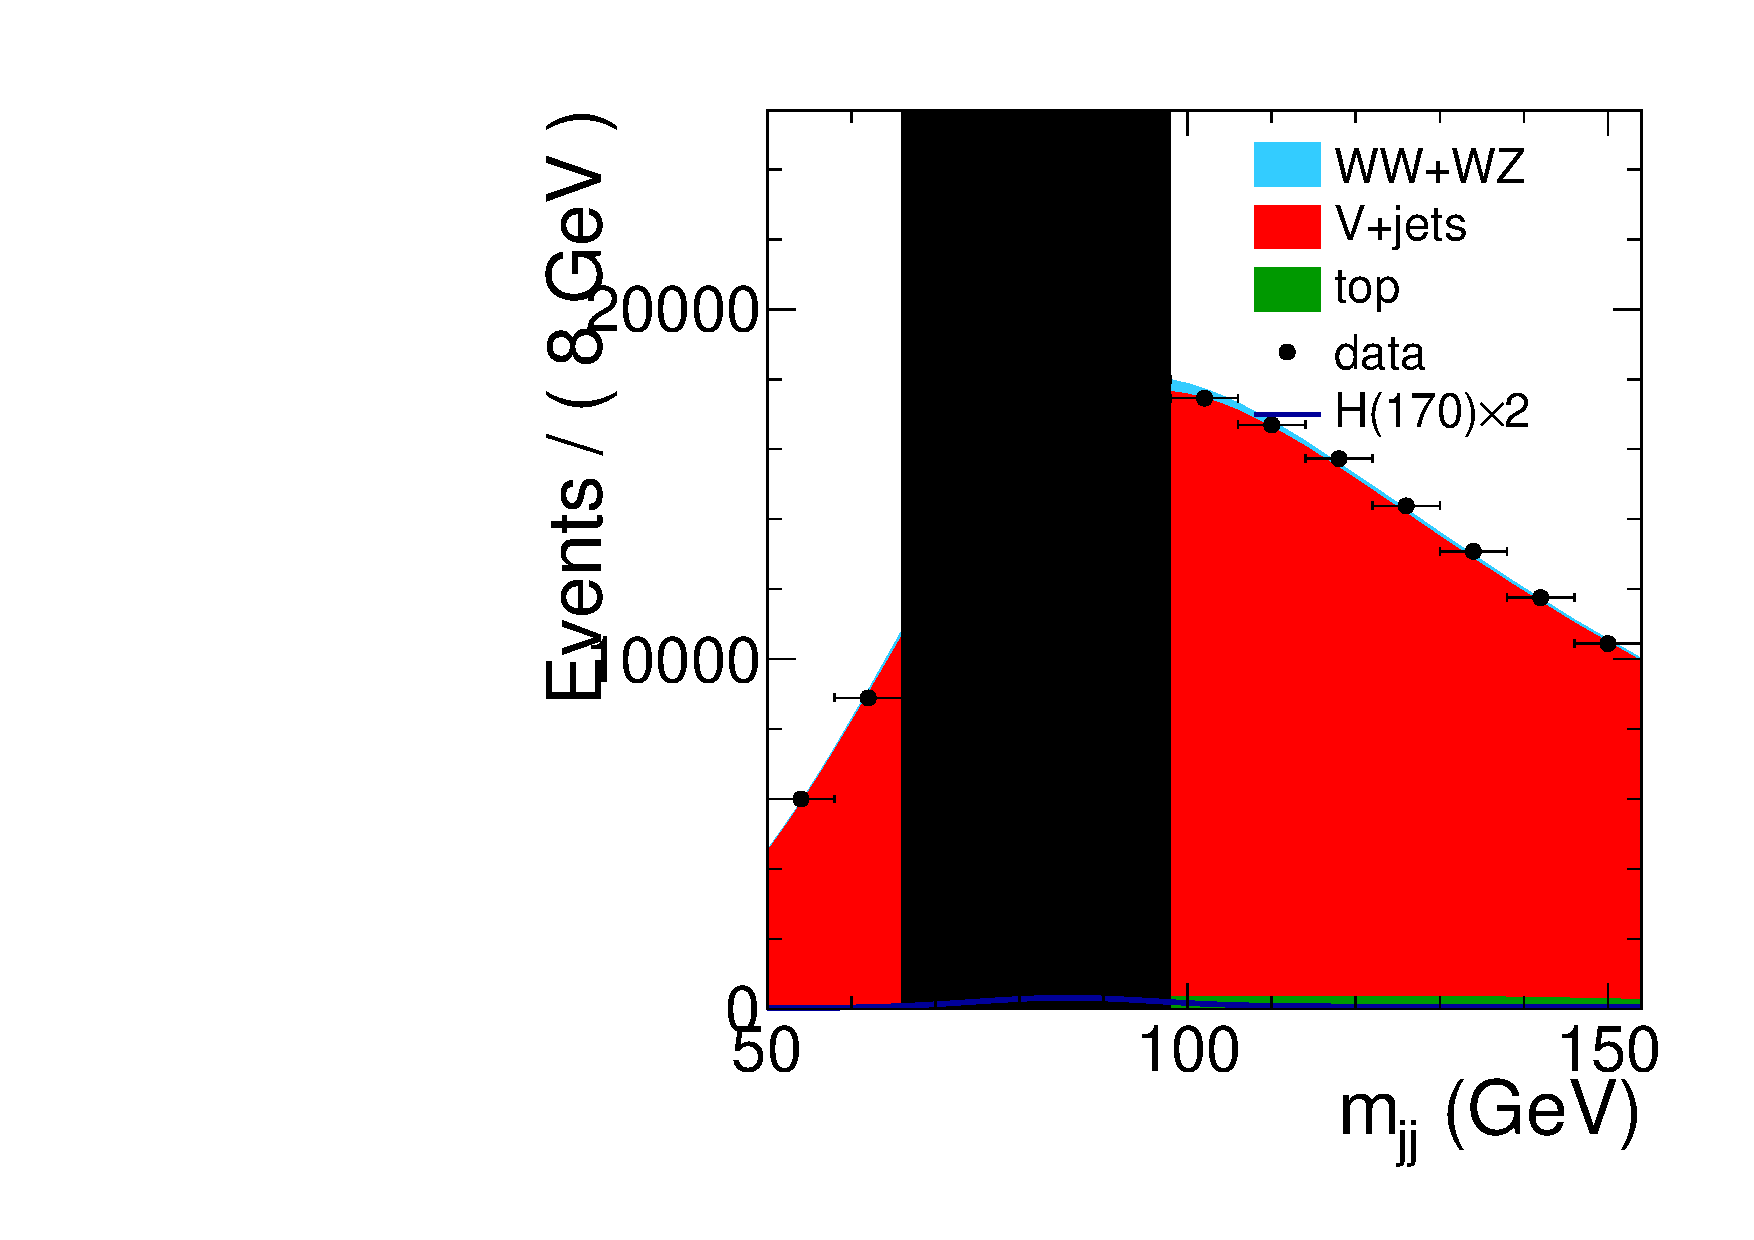
\includegraphics[width=0.49\textwidth]{plots/2012_FOURBSHAPES/HWW170lnujj_muon_mjj_stacked}
  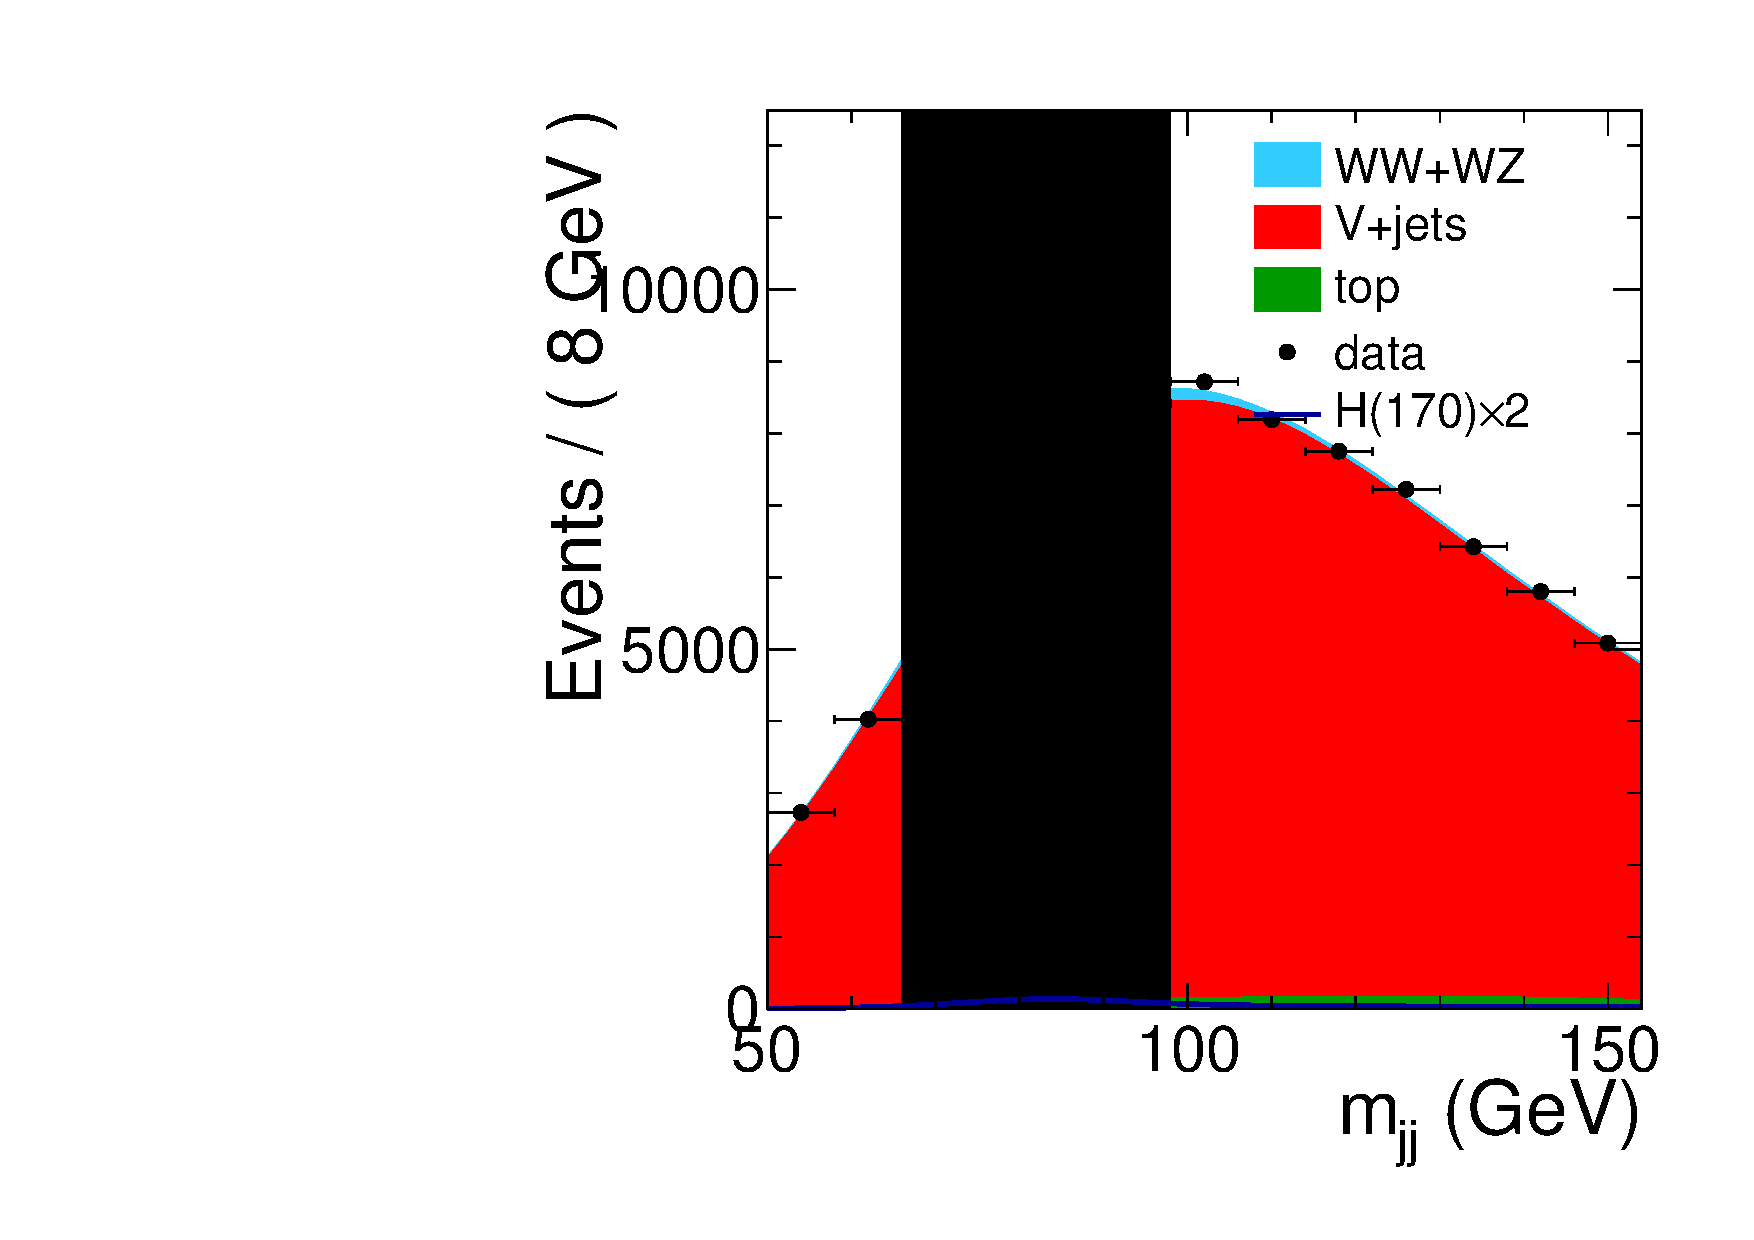
\includegraphics[width=0.49\textwidth]{plots/2012_FOURBSHAPES/HWW170lnujj_electron_mjj_stacked}
  %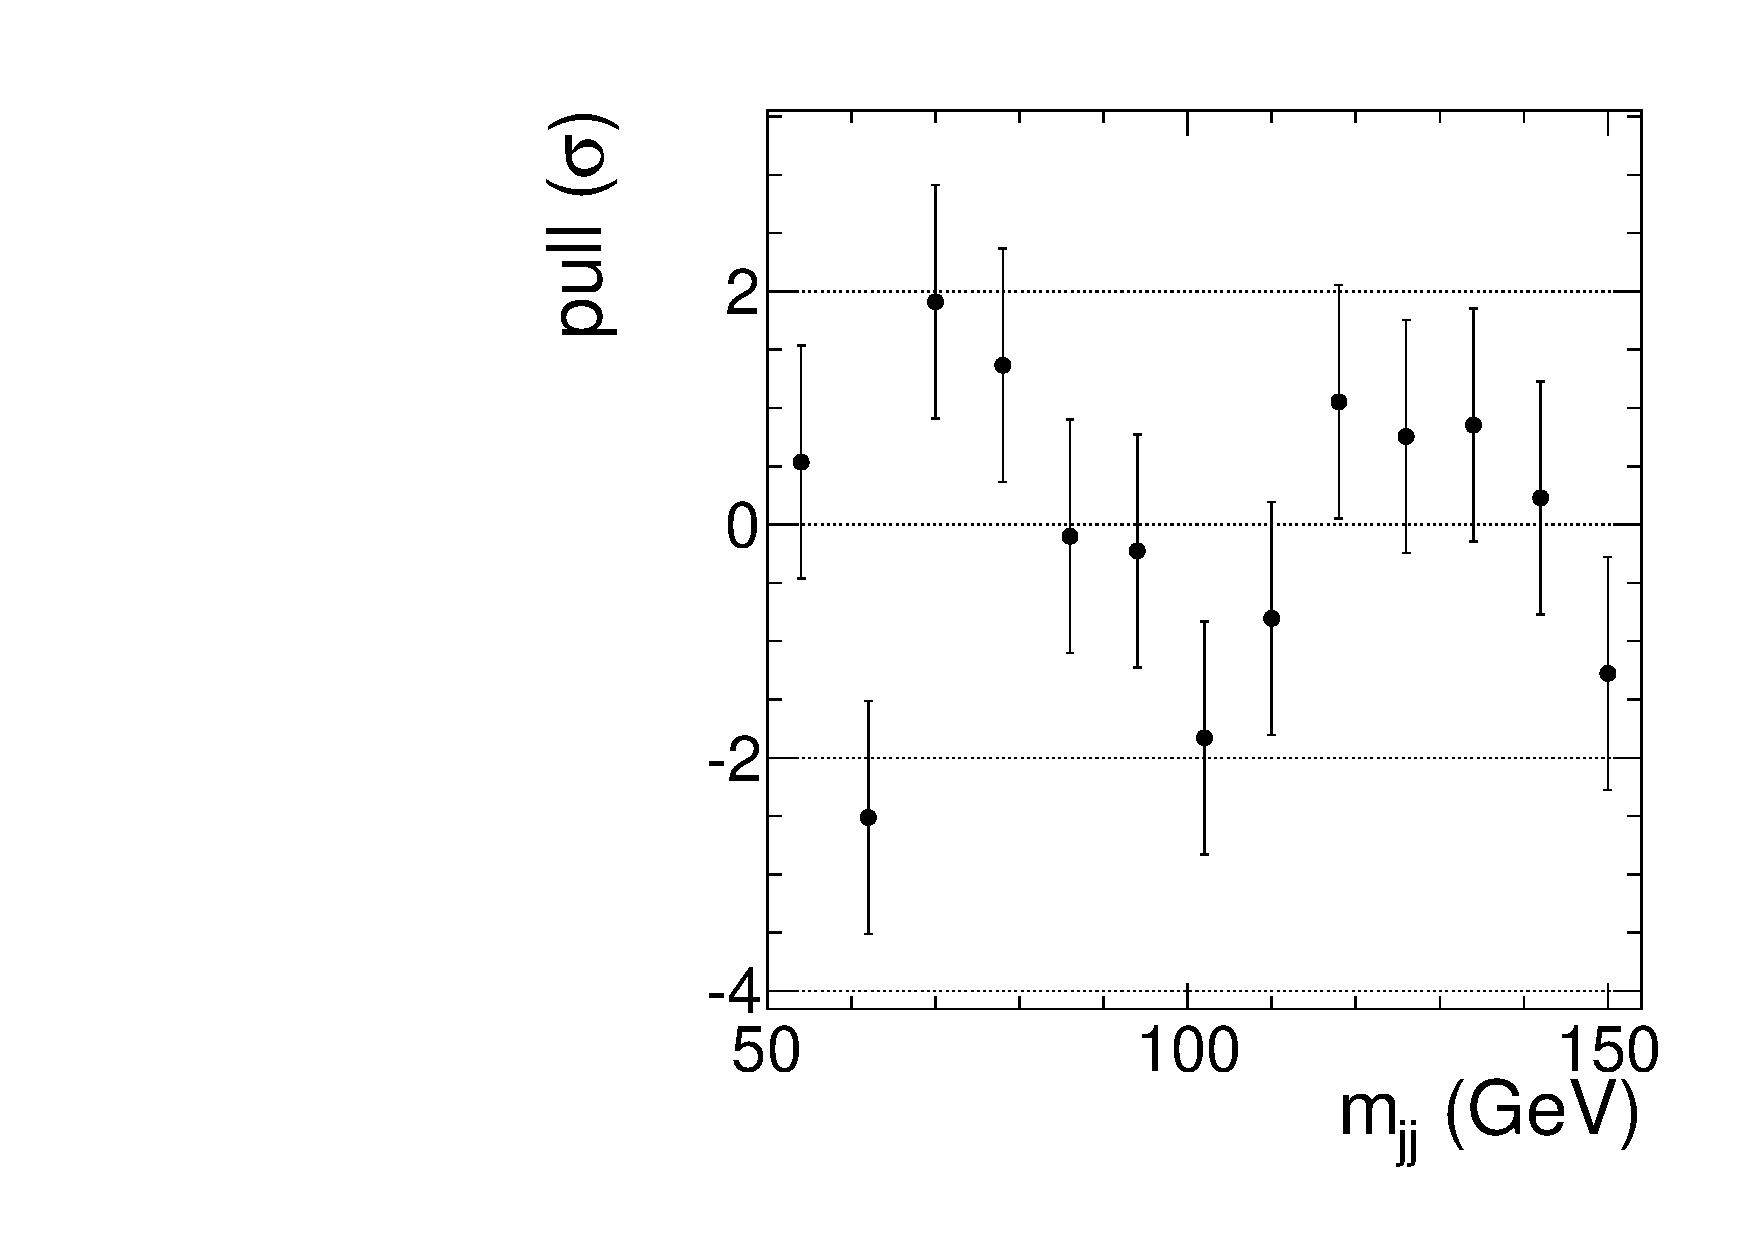
\includegraphics[width=0.49\textwidth]{plots/2012_FOURBSHAPES/HWW170lnujj_muon_mjj_pull}
  % \parbox[b][0.49\textwidth][r]{0.49\textwidth}{pull to be included when unblinded.}
  \caption{\label{fig:mjj_mH170}For the SM Higgs mass of 170~GeV, the
    distribution of the dijet invariant mass $m_{jj}$ is shown with
    muons on the left and electrons on the right.}
  % The pull
  %   distribution computed as [(Data - Fit)/ Fit uncertainty] is shown
  %   on the right. } %% The signal region is blinded.}
\end{figure}

\begin{figure}[!t]
  \centering
  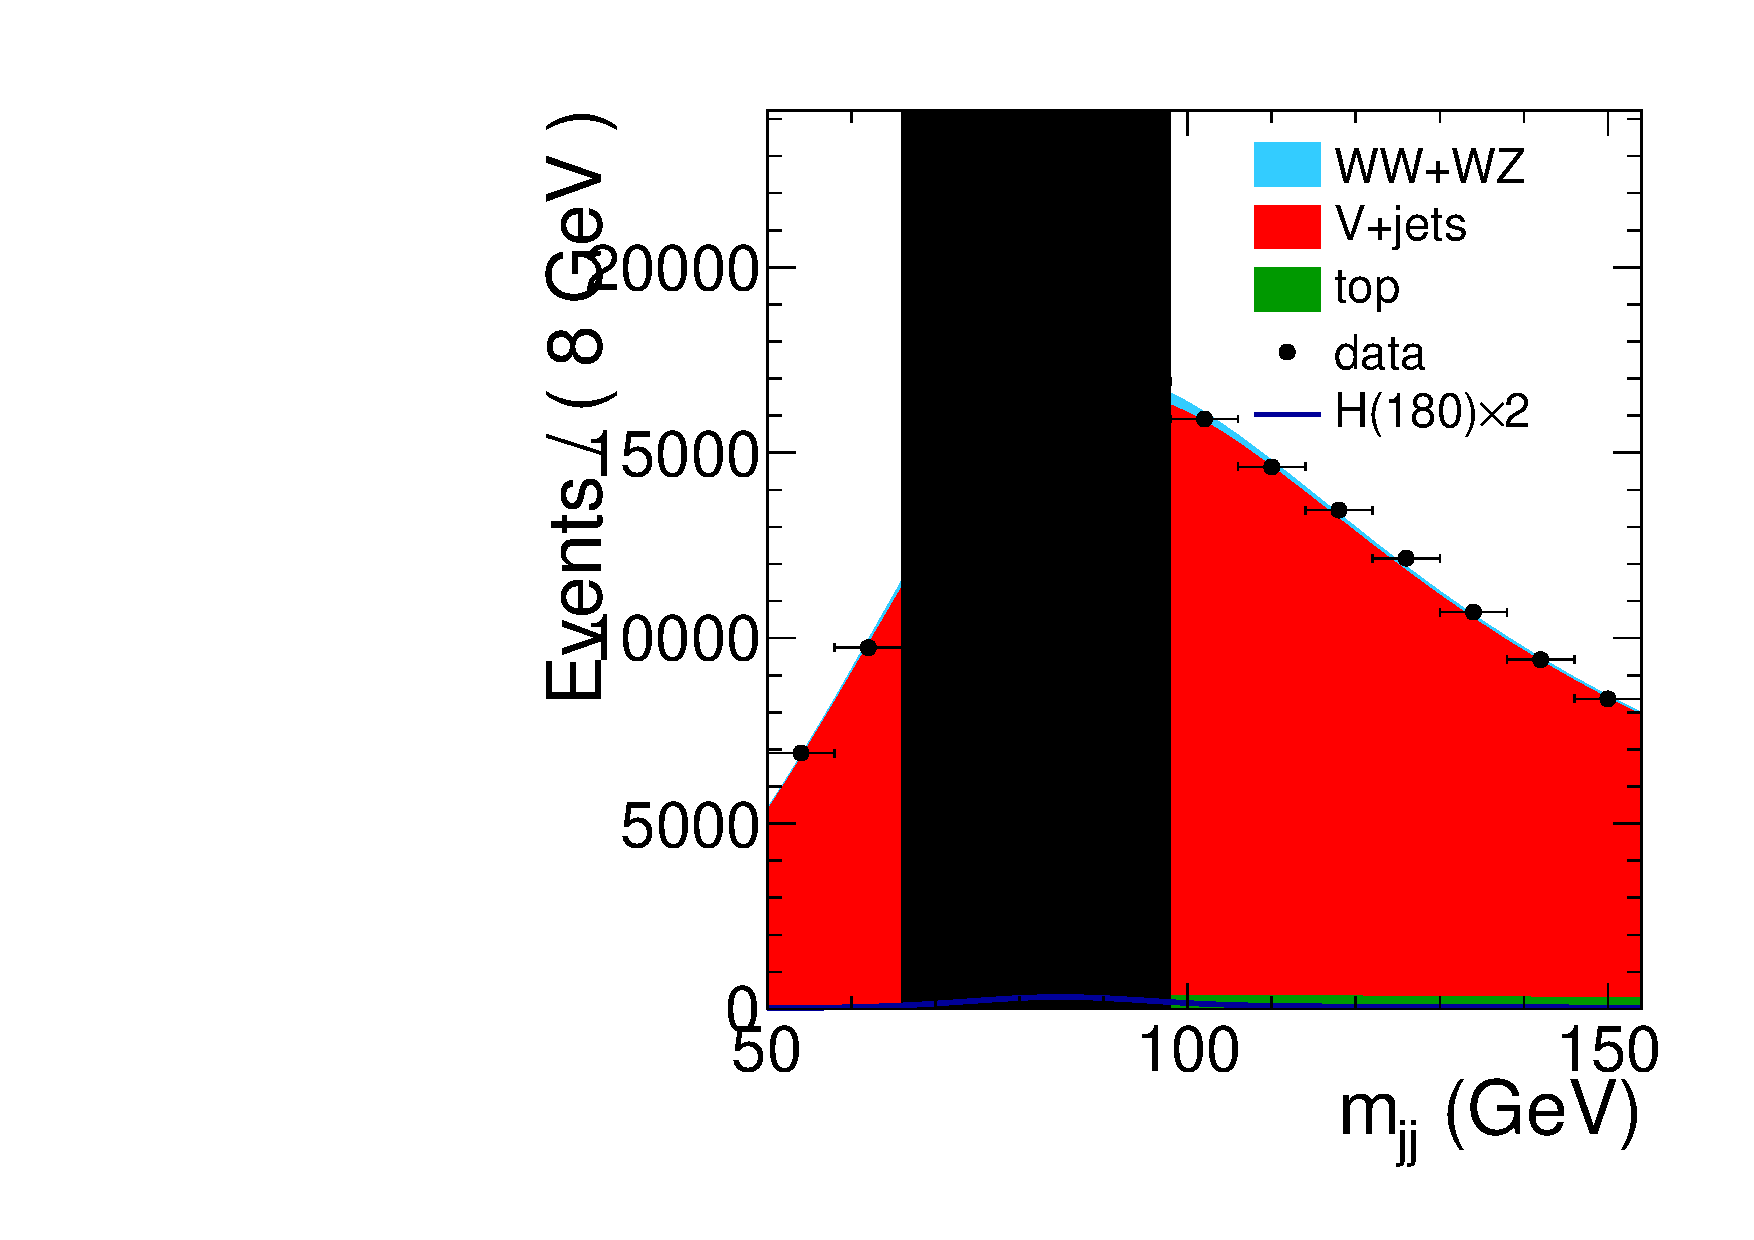
\includegraphics[width=0.49\textwidth]{plots/2012_FOURBSHAPES/HWW180lnujj_muon_mjj_stacked}
  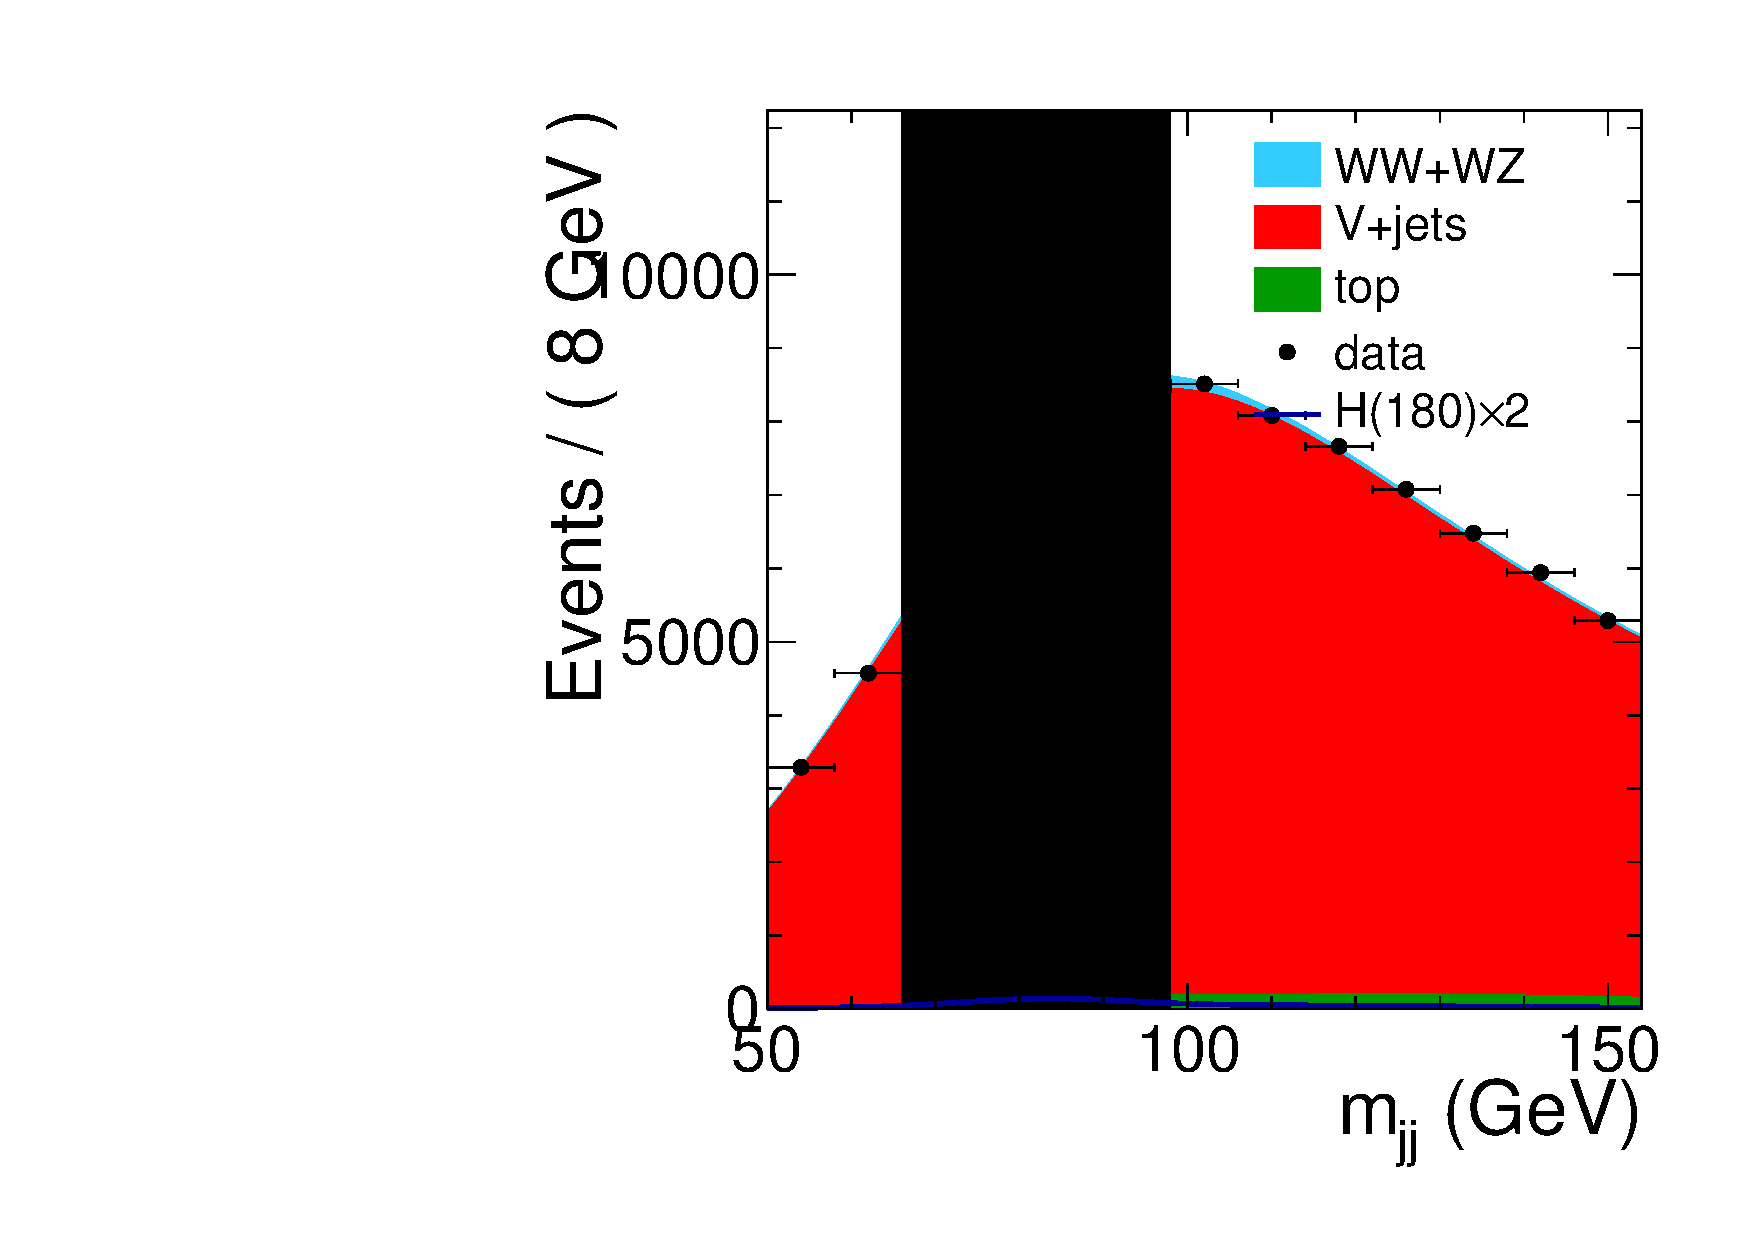
\includegraphics[width=0.49\textwidth]{plots/2012_FOURBSHAPES/HWW180lnujj_electron_mjj_stacked}
  %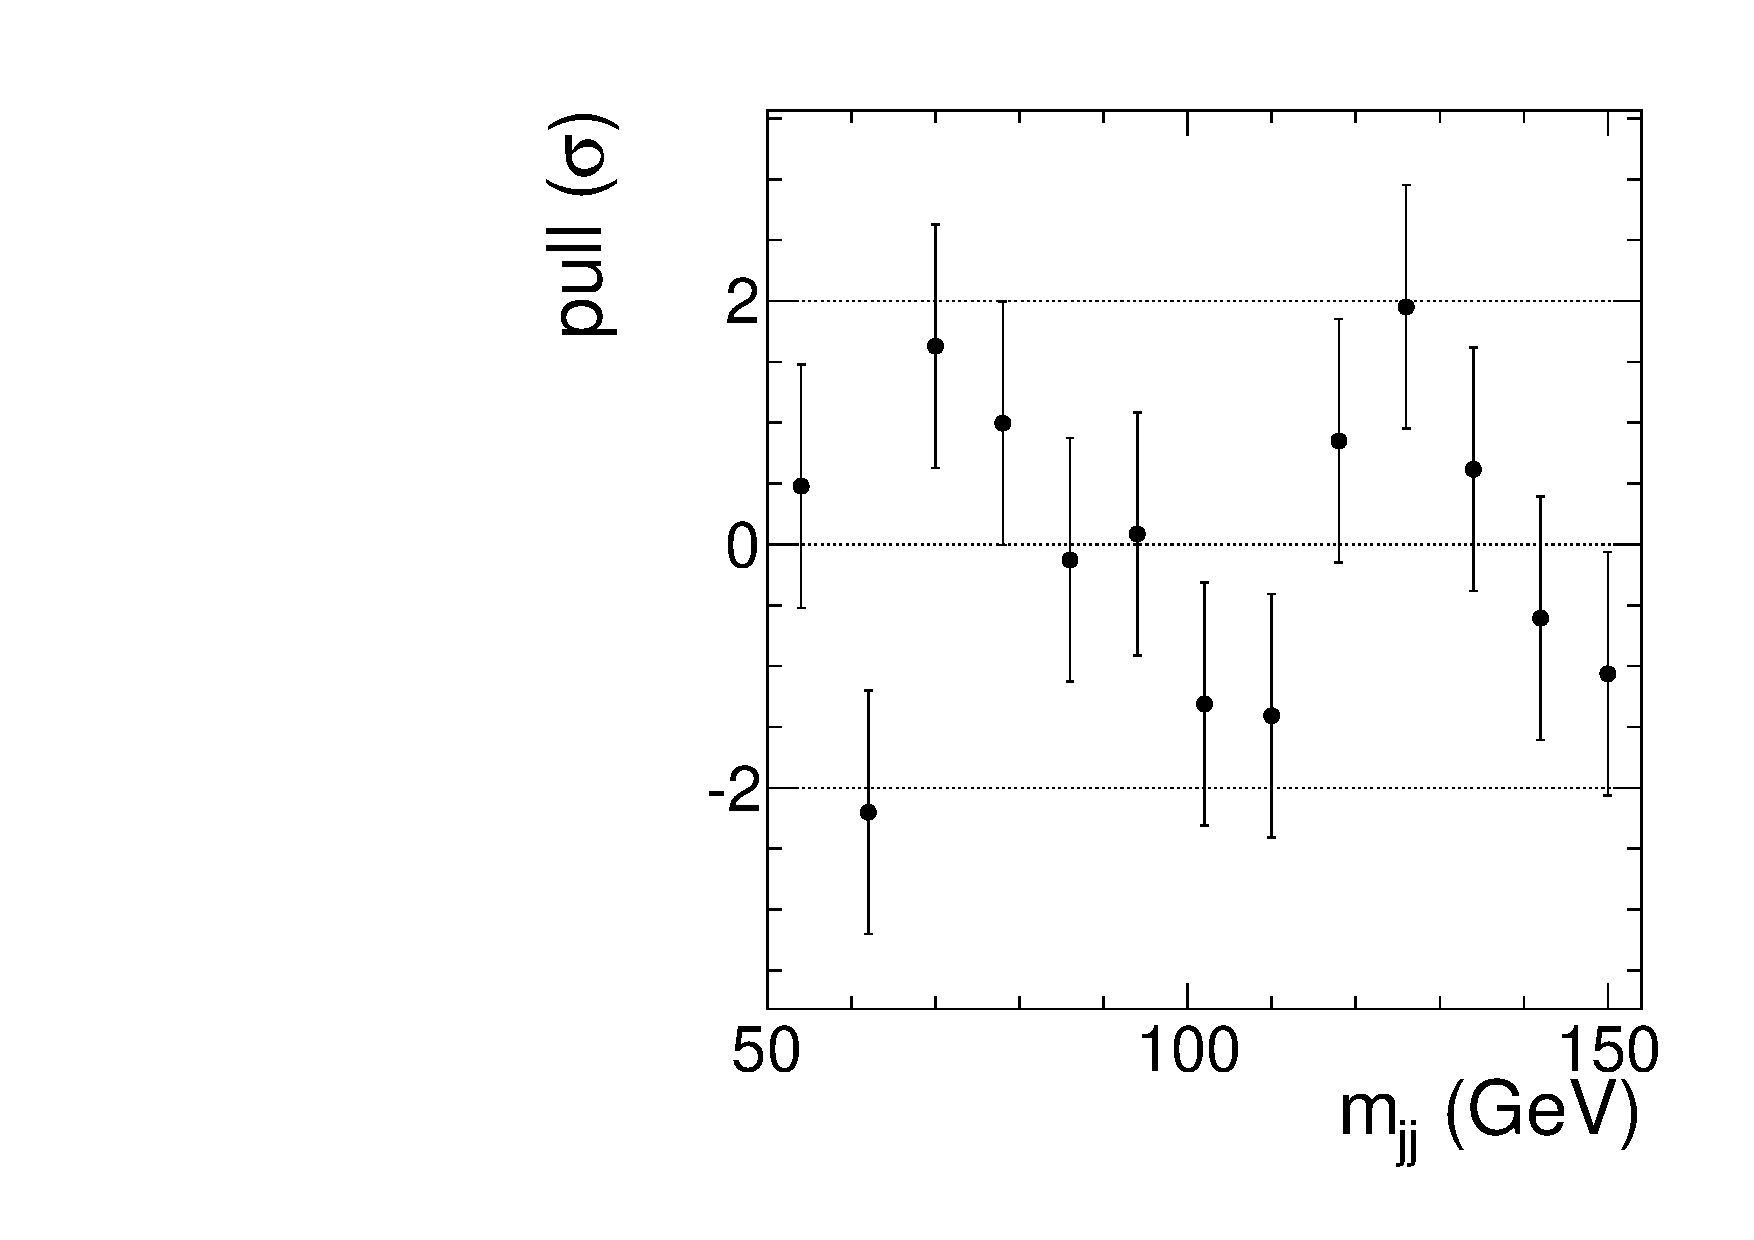
\includegraphics[width=0.49\textwidth]{plots/2012_FOURBSHAPES/HWW180lnujj_muon_mjj_pull}
  % \parbox[b][0.49\textwidth][r]{0.49\textwidth}{pull to be included when unblinded.}
  \caption{\label{fig:mjj_mH180}For the SM Higgs mass of 180~GeV, the
    distribution of the dijet invariant mass $m_{jj}$ is shown with
    muons on the left and electrons on the right.}
  % The pull
  %   distribution computed as [(Data - Fit)/ Fit uncertainty] is shown
  %   on the right. } %% The signal region is blinded.}
\end{figure}

\begin{figure}[!t]
  \centering
  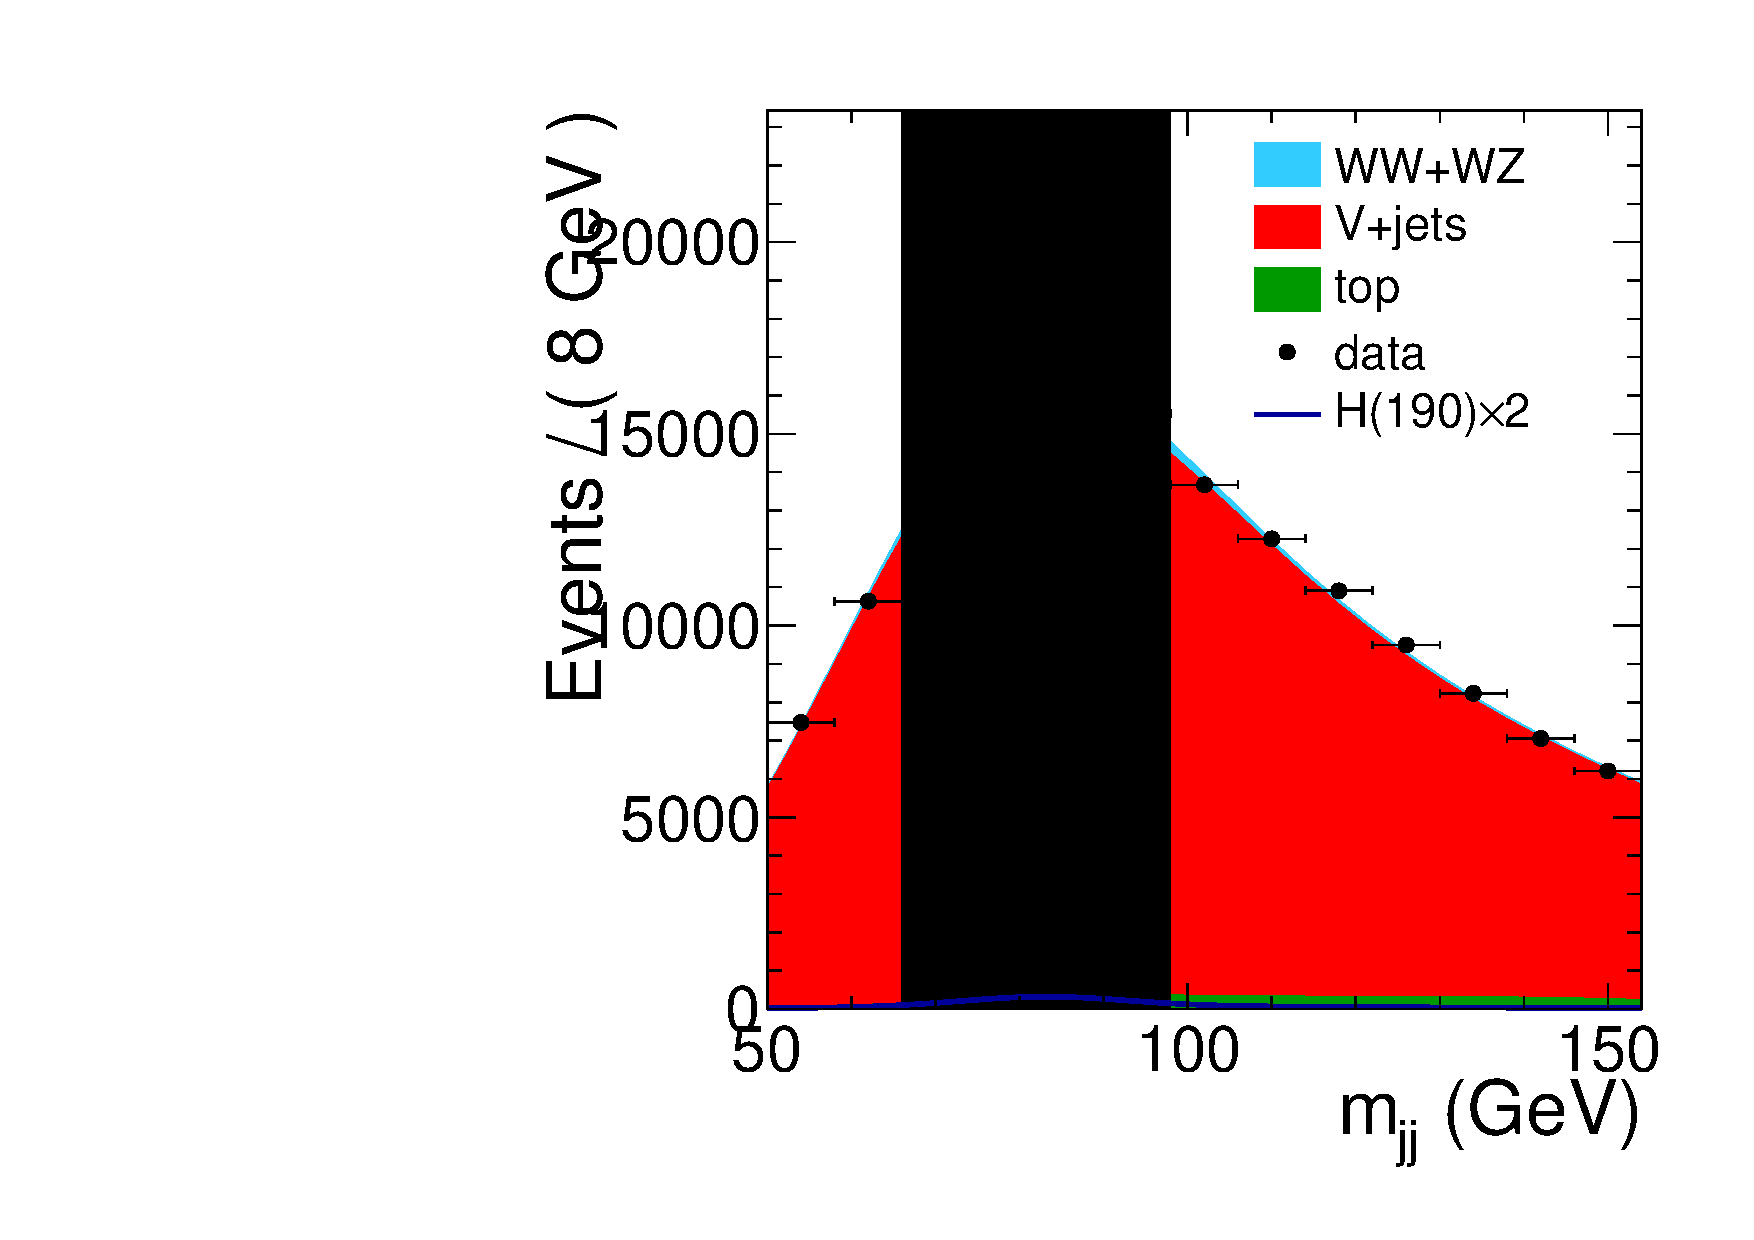
\includegraphics[width=0.49\textwidth]{plots/2012_FOURBSHAPES/HWW190lnujj_muon_mjj_stacked}
  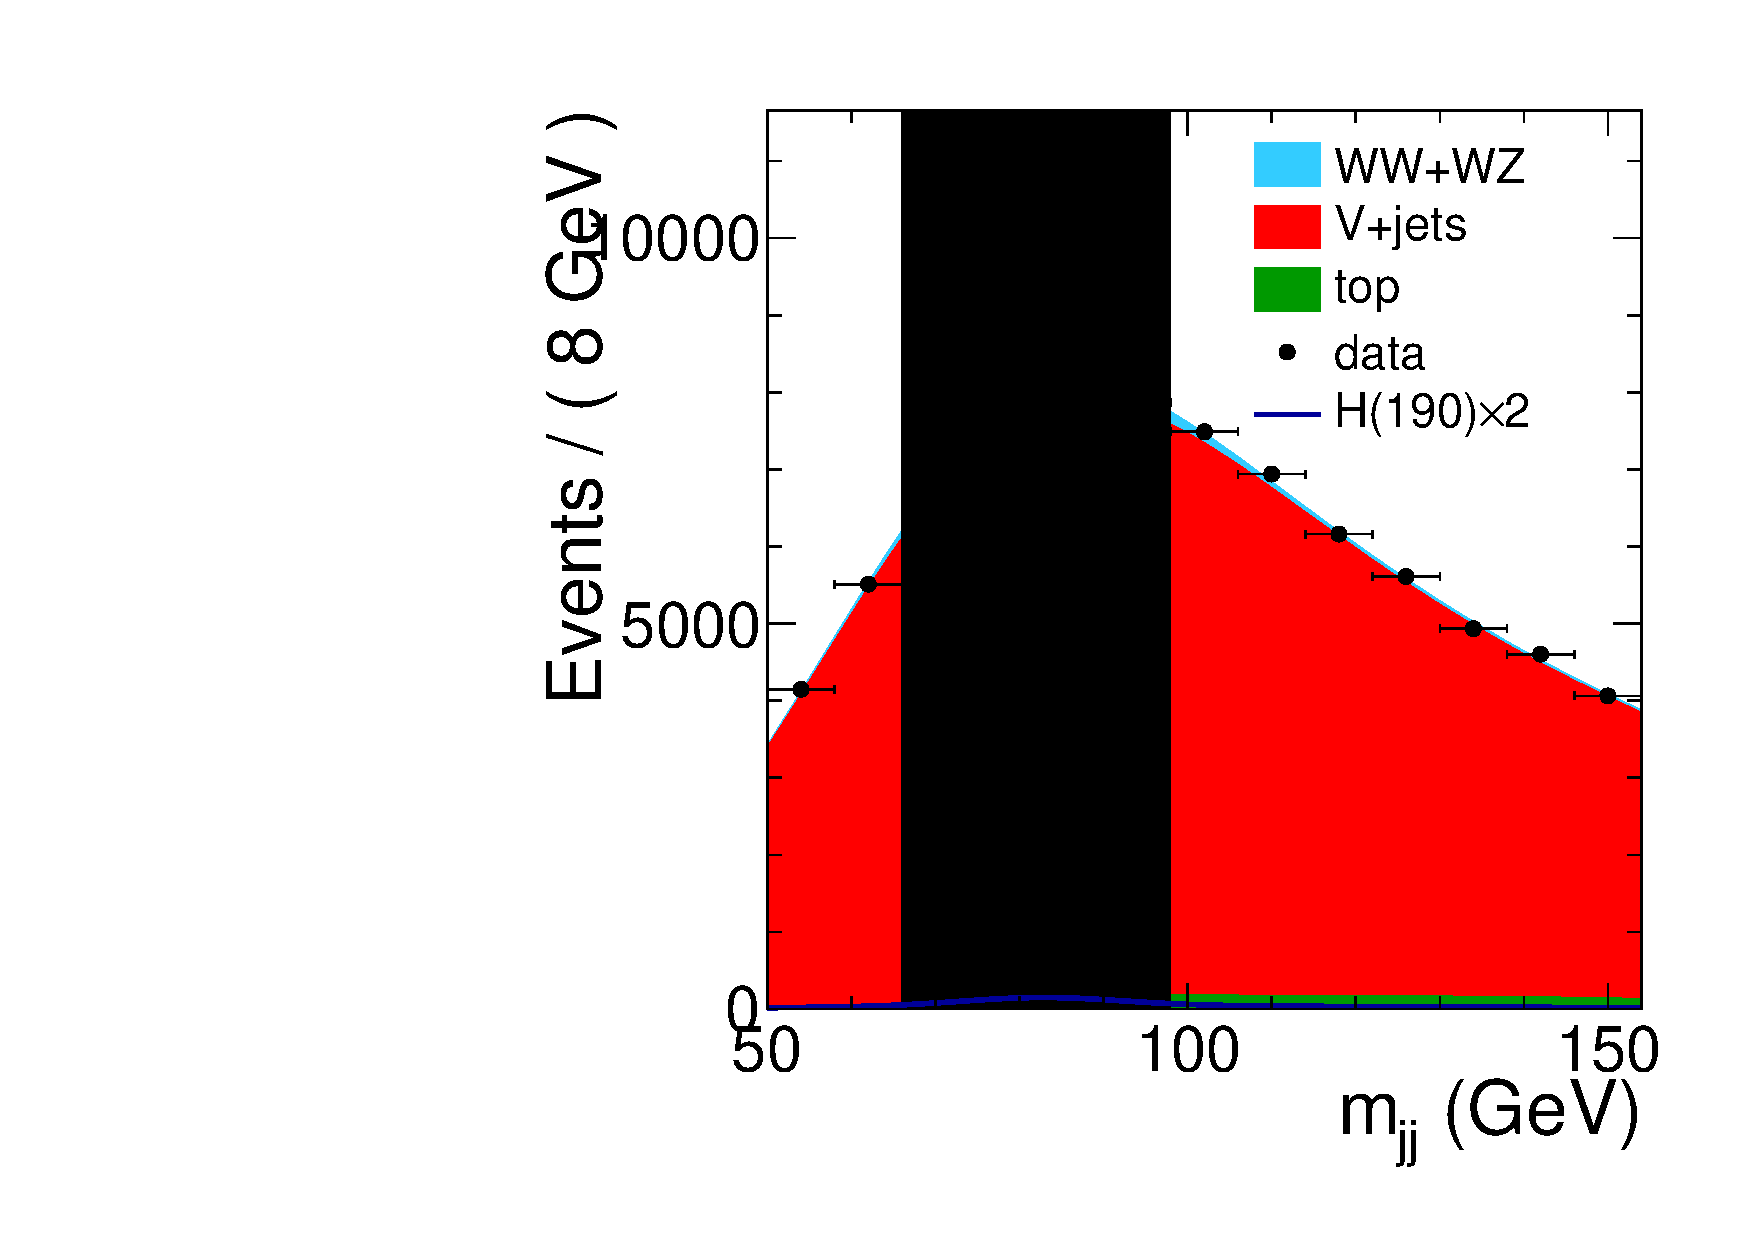
\includegraphics[width=0.49\textwidth]{plots/2012_FOURBSHAPES/HWW190lnujj_electron_mjj_stacked}
  %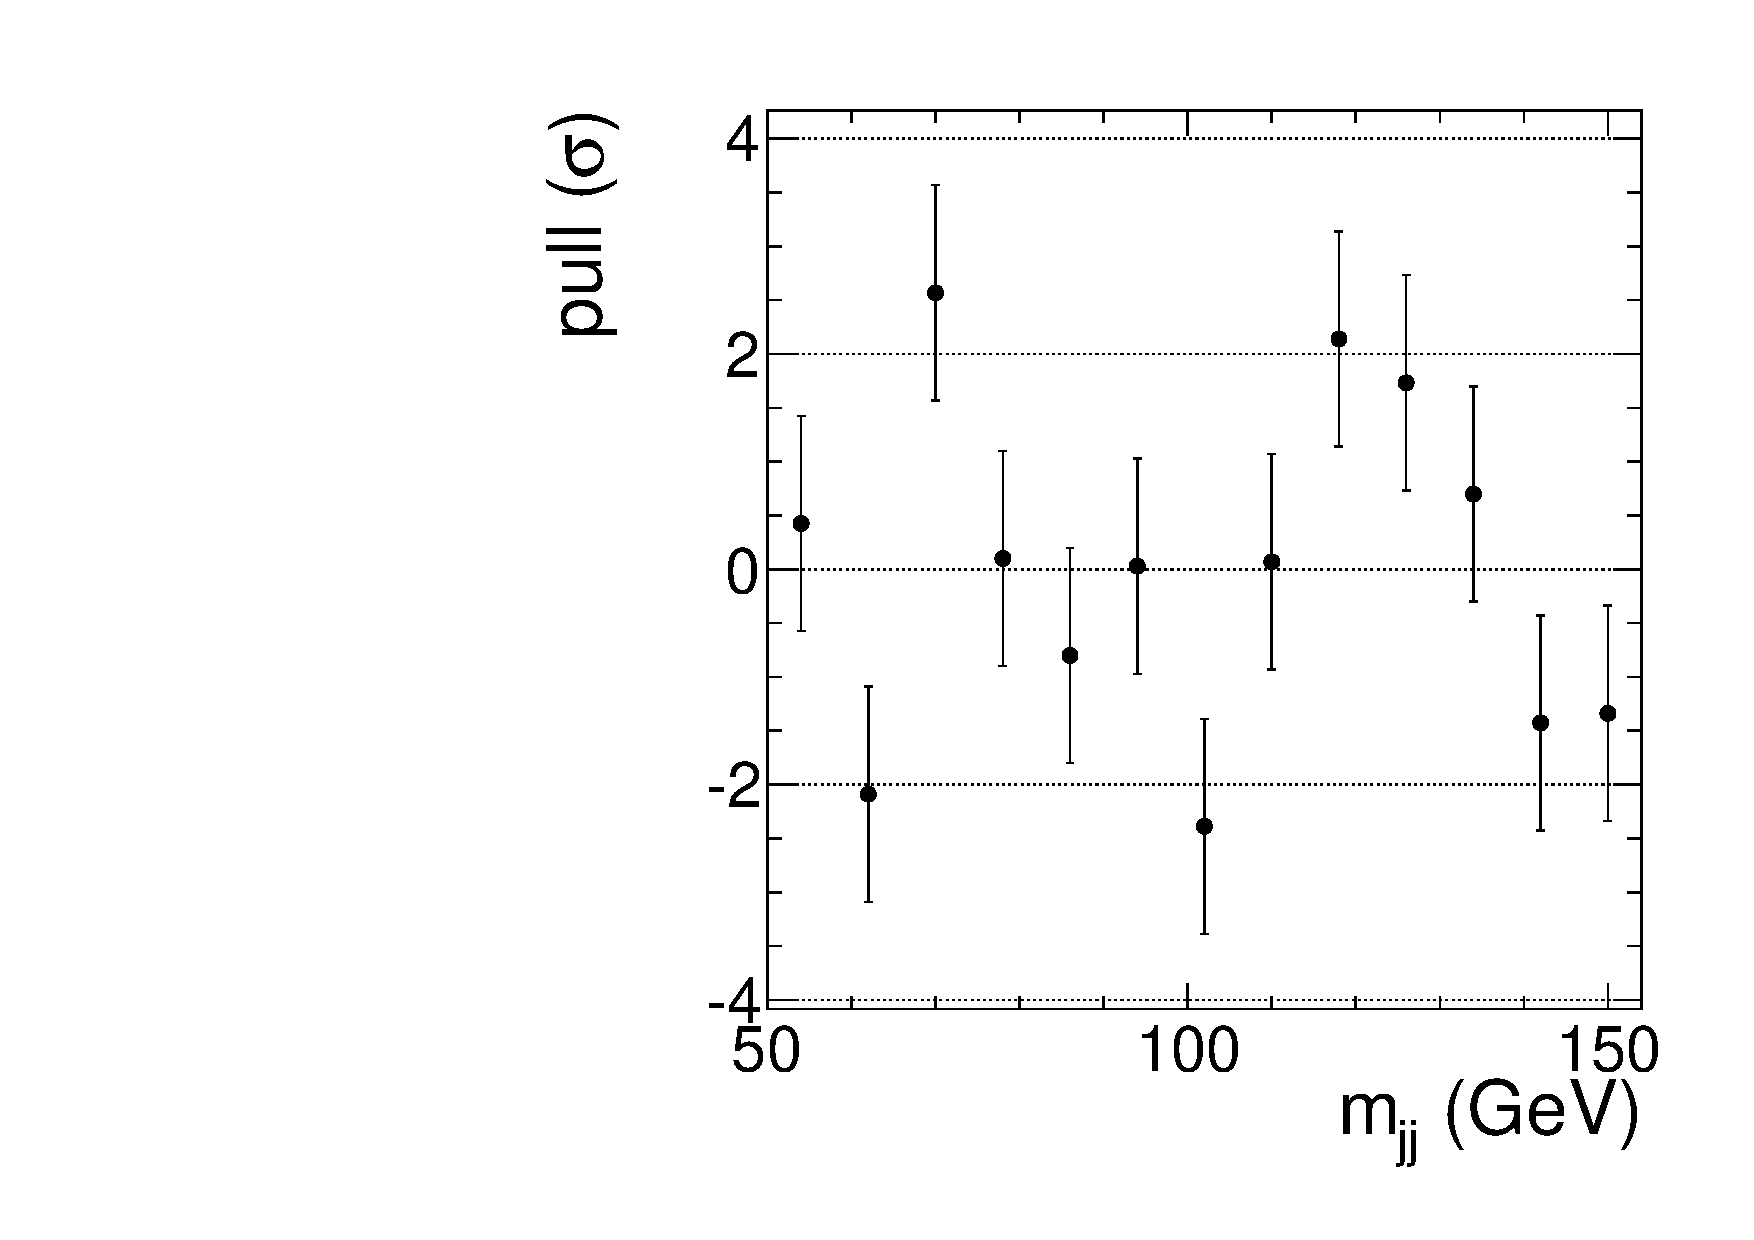
\includegraphics[width=0.49\textwidth]{plots/2012_FOURBSHAPES/HWW190lnujj_muon_mjj_pull}
  % \parbox[b][0.49\textwidth][r]{0.49\textwidth}{pull to be included when unblinded.}
  \caption{\label{fig:mjj_mH190}For the SM Higgs mass of 190~GeV, the
    distribution of the dijet invariant mass $m_{jj}$ is shown with
    muons on the left and electrons on the right.}
  % The pull
  %   distribution computed as [(Data - Fit)/ Fit uncertainty] is shown
  %   on the right. } %% The signal region is blinded.}
\end{figure}

\begin{figure}[!t]
  \centering
  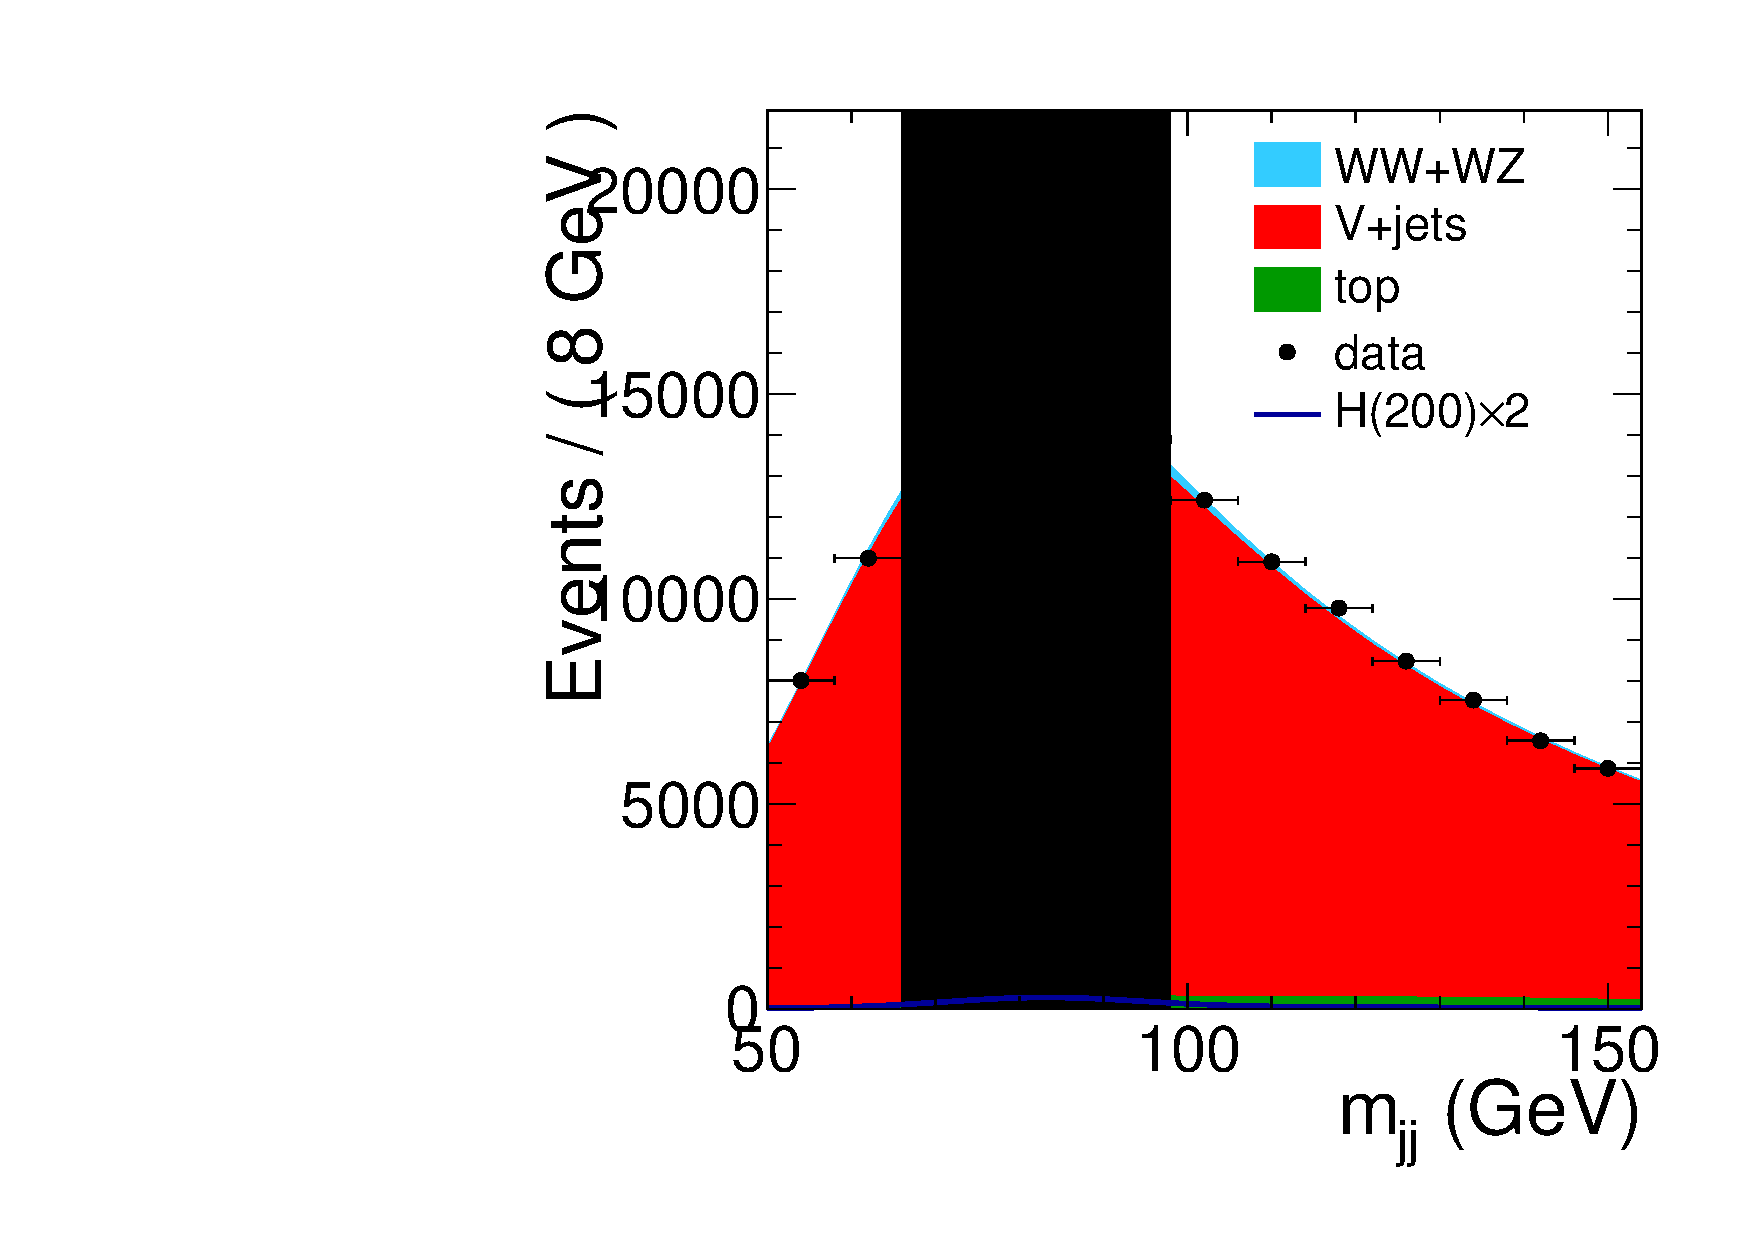
\includegraphics[width=0.49\textwidth]{plots/2012_FOURBSHAPES/HWW200lnujj_muon_mjj_stacked}
  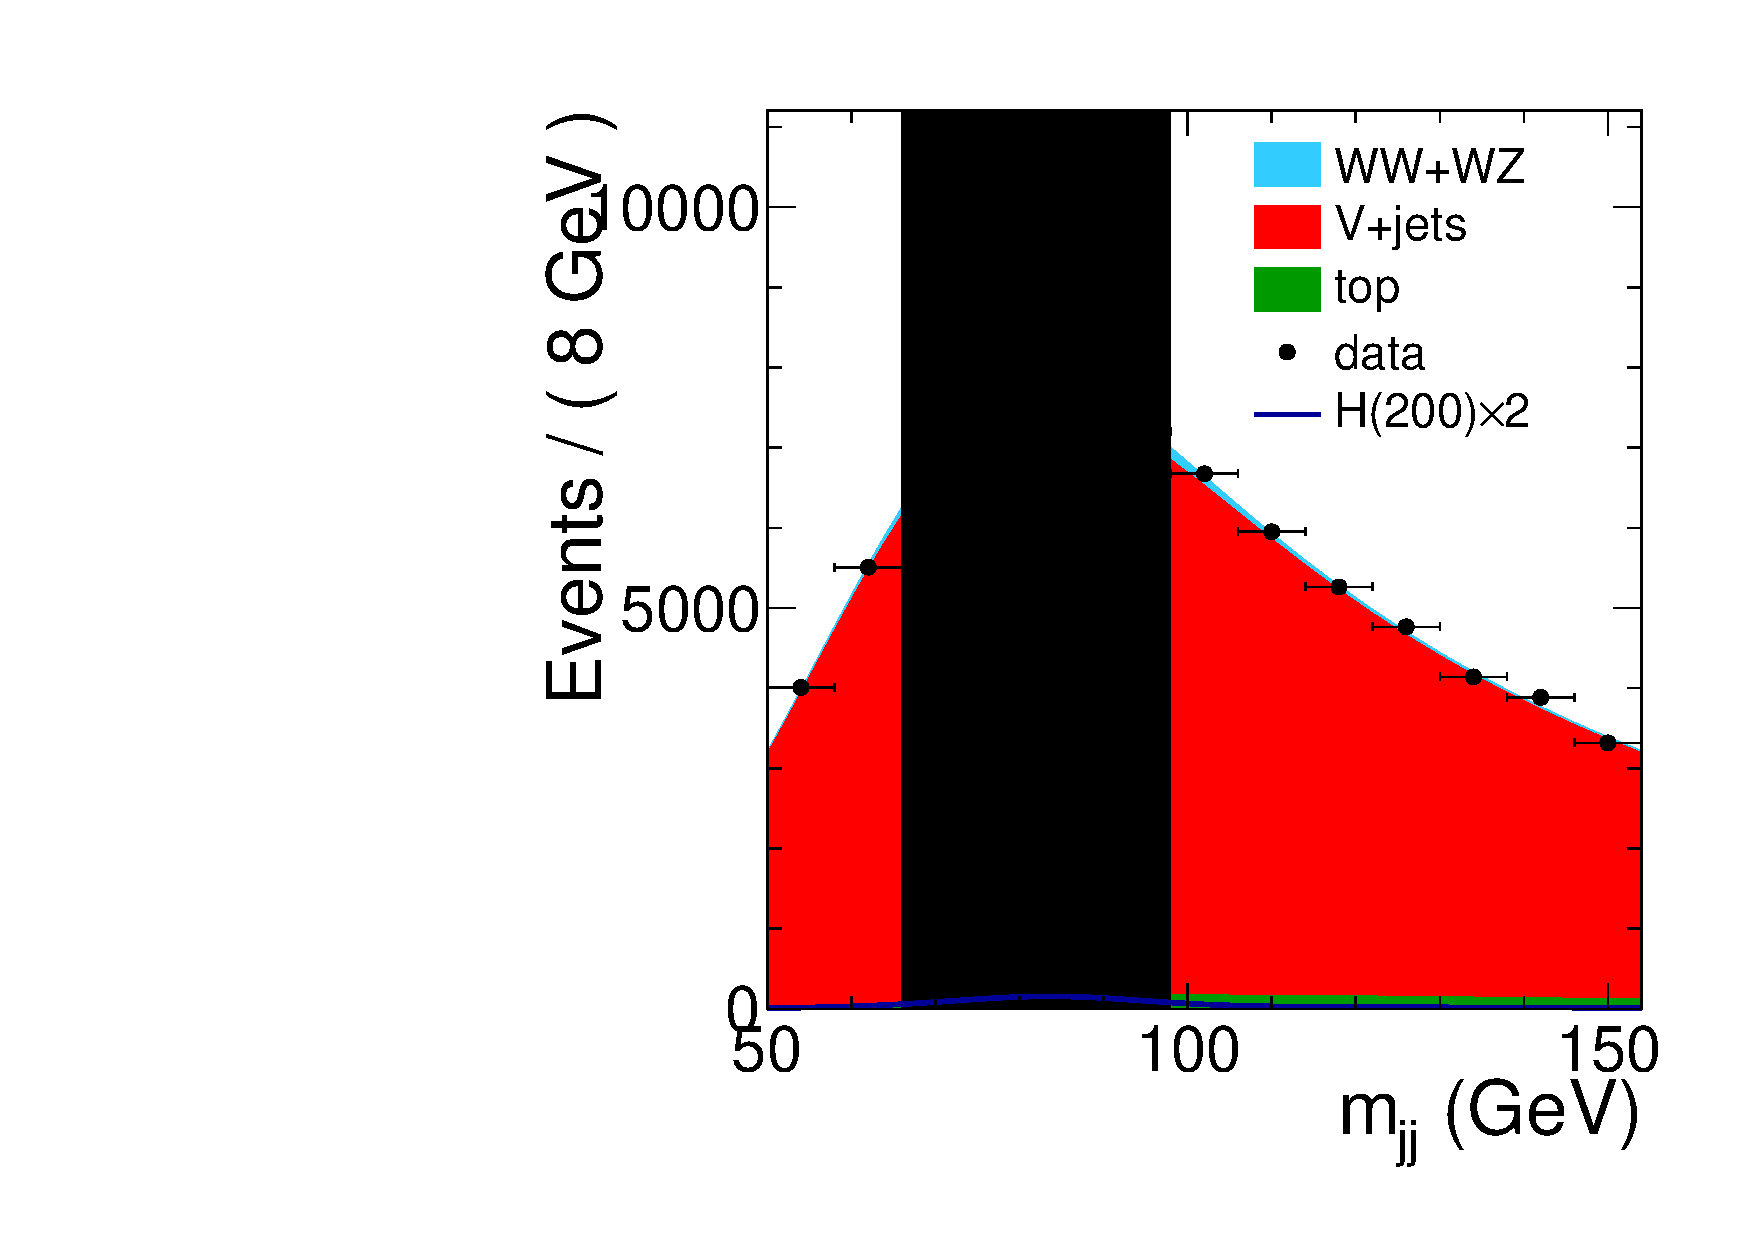
\includegraphics[width=0.49\textwidth]{plots/2012_FOURBSHAPES/HWW200lnujj_electron_mjj_stacked}
  %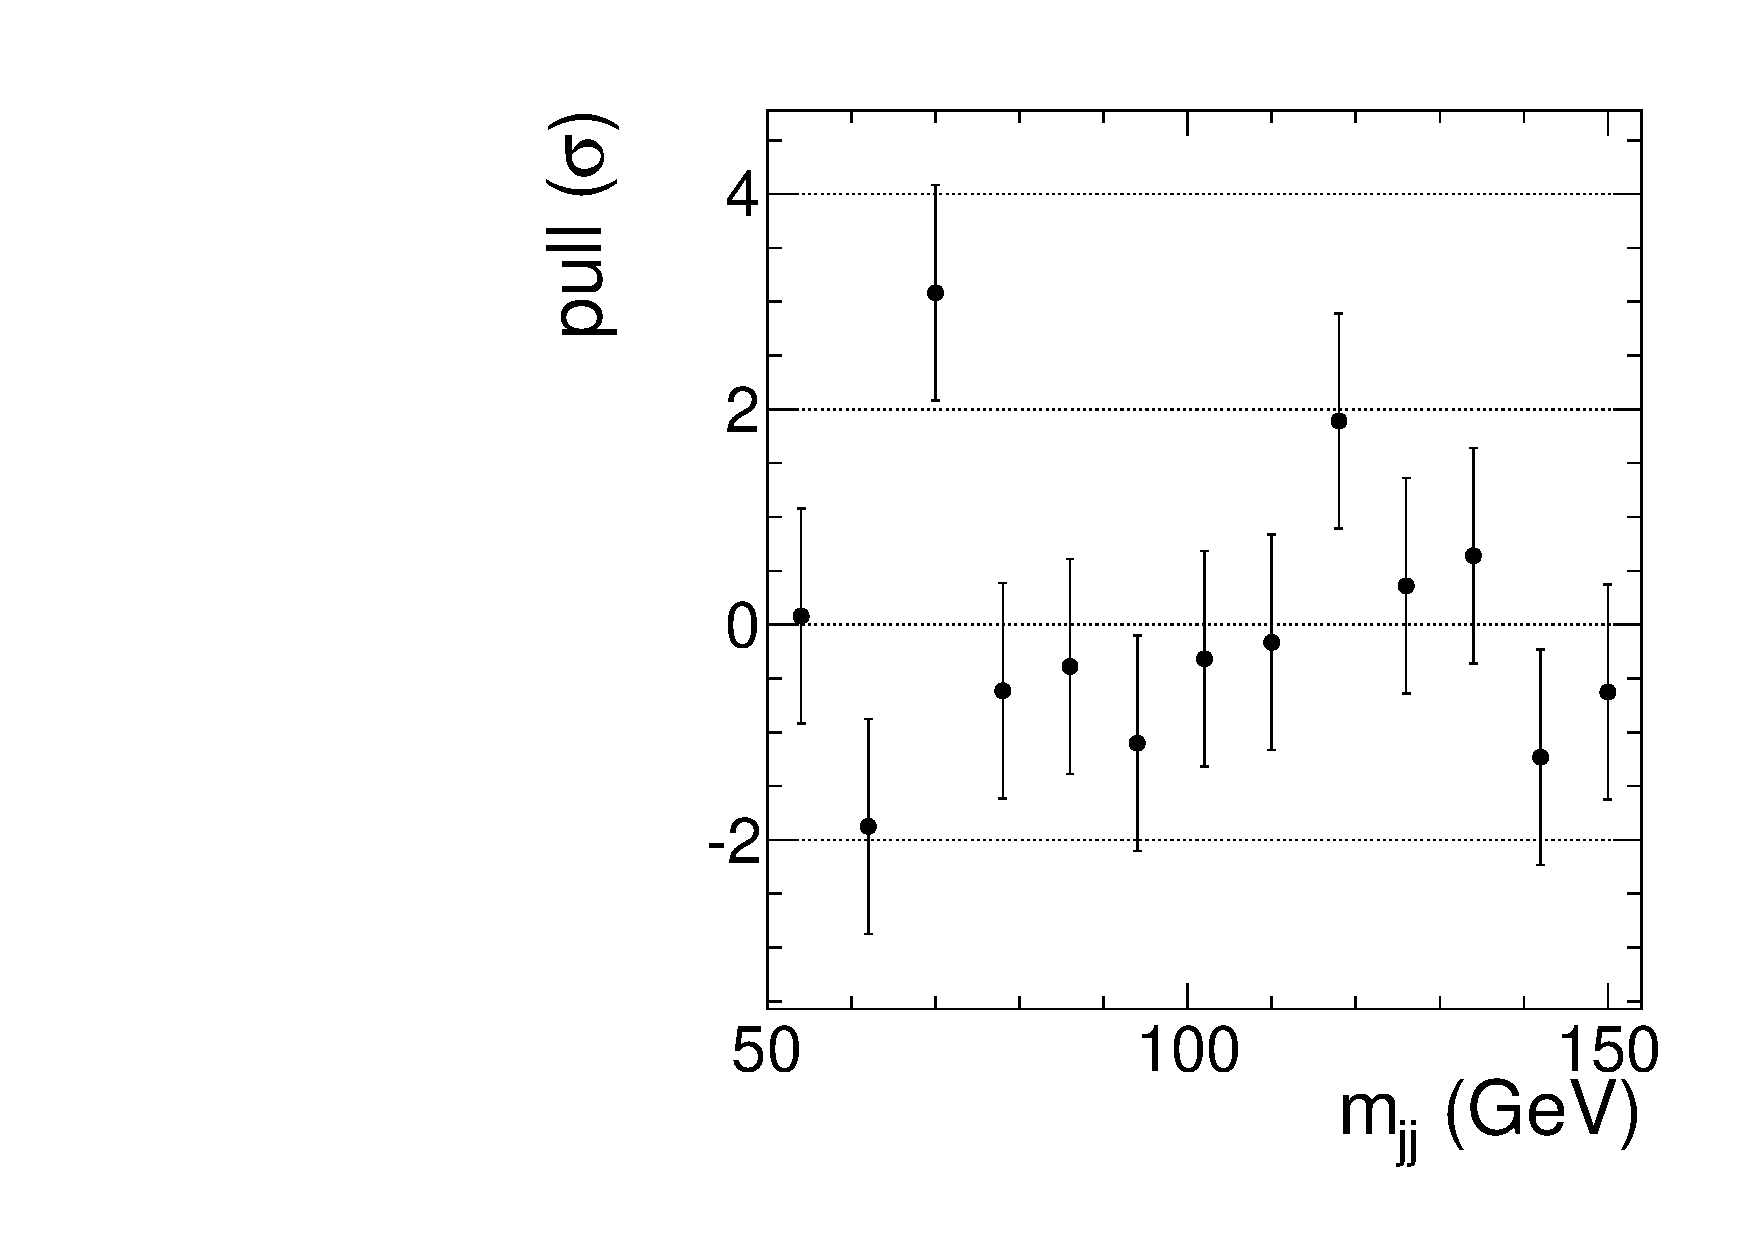
\includegraphics[width=0.49\textwidth]{plots/2012_FOURBSHAPES/HWW200lnujj_muon_mjj_pull}
  % \parbox[b][0.49\textwidth][r]{0.49\textwidth}{pull to be included when unblinded.}
  \caption{\label{fig:mjj_mH200}For the SM Higgs mass of 200~GeV, the
    distribution of the dijet invariant mass $m_{jj}$ is shown with
    muons on the left and electrons on the right.}
  % The pull
  %   distribution computed as [(Data - Fit)/ Fit uncertainty] is shown
  %   on the right. } %% The signal region is blinded.}
\end{figure}

\begin{figure}[!t]
  \centering
  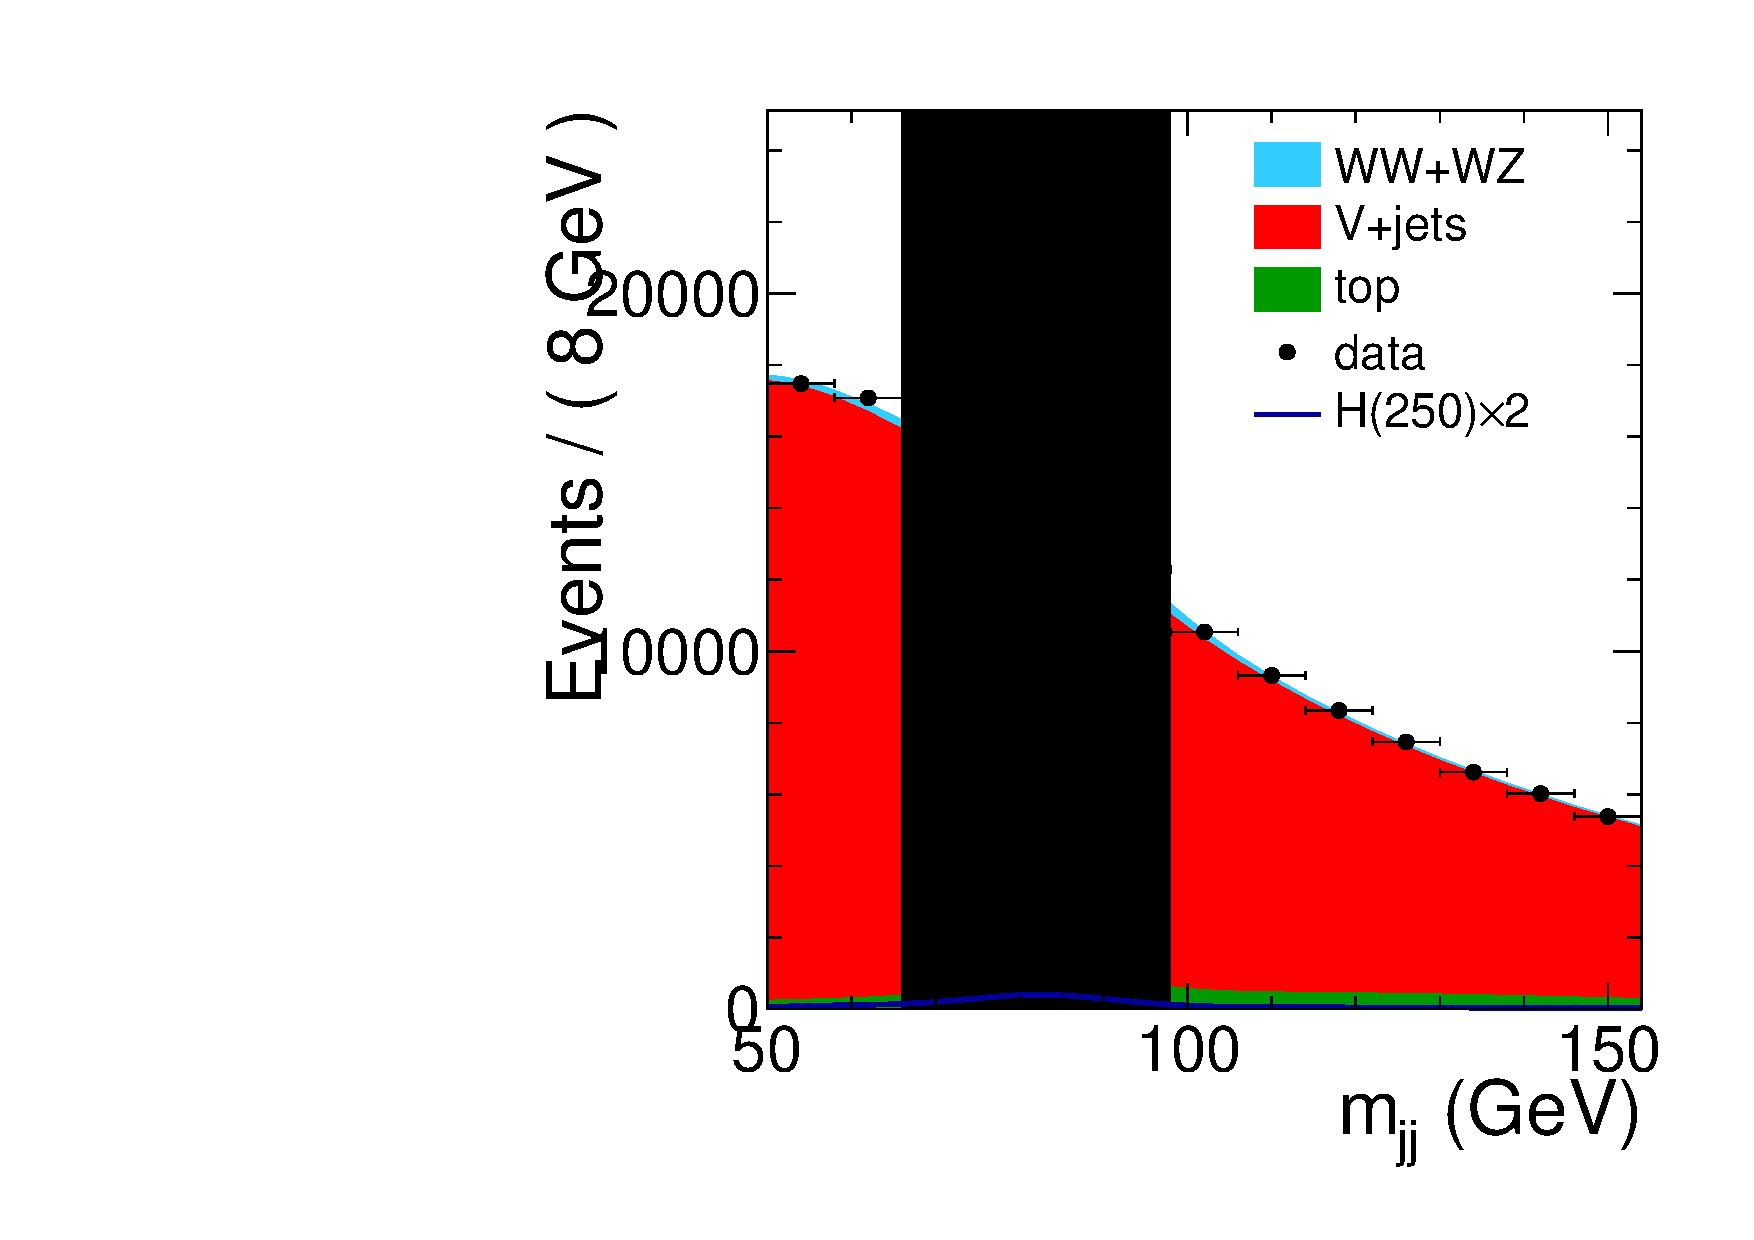
\includegraphics[width=0.49\textwidth]{plots/2012_FOURBSHAPES/HWW250lnujj_muon_mjj_stacked}
  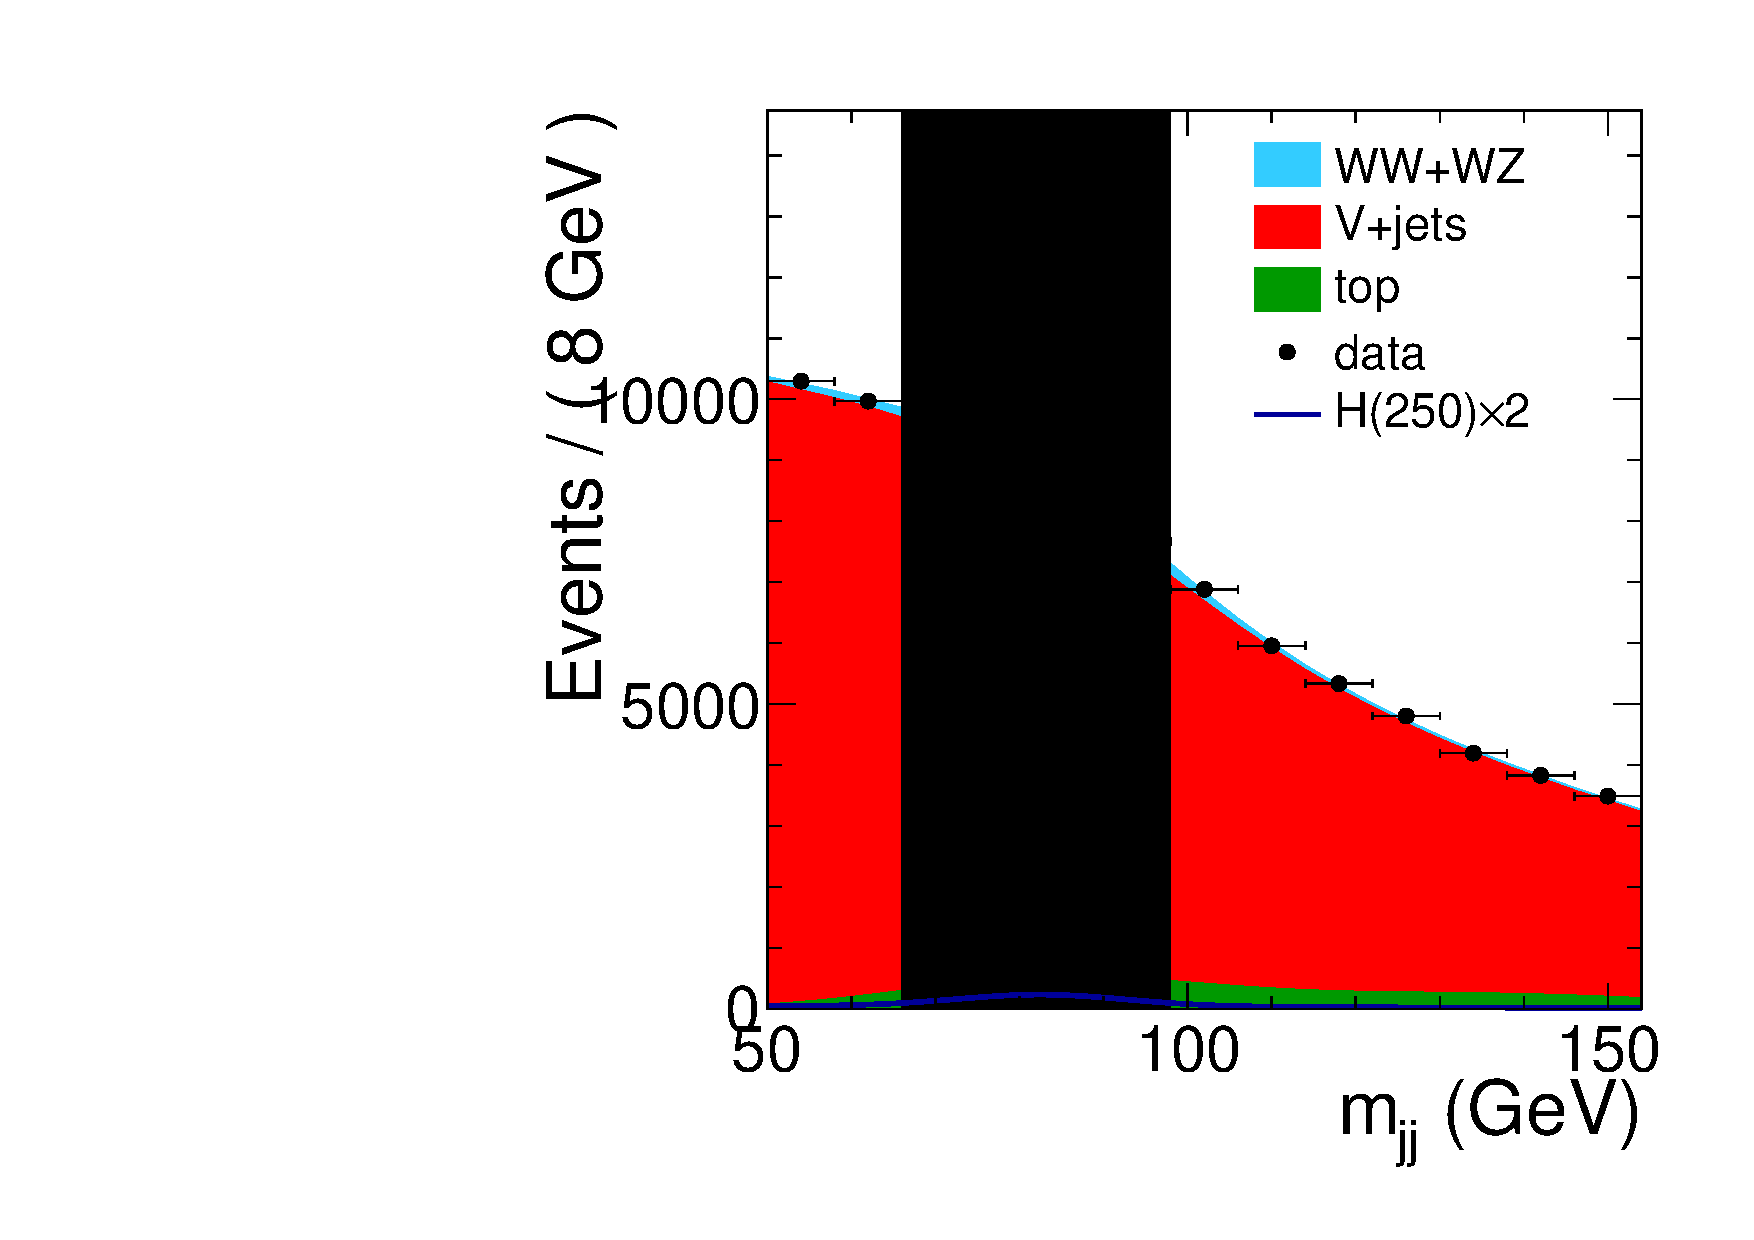
\includegraphics[width=0.49\textwidth]{plots/2012_FOURBSHAPES/HWW250lnujj_electron_mjj_stacked}
  %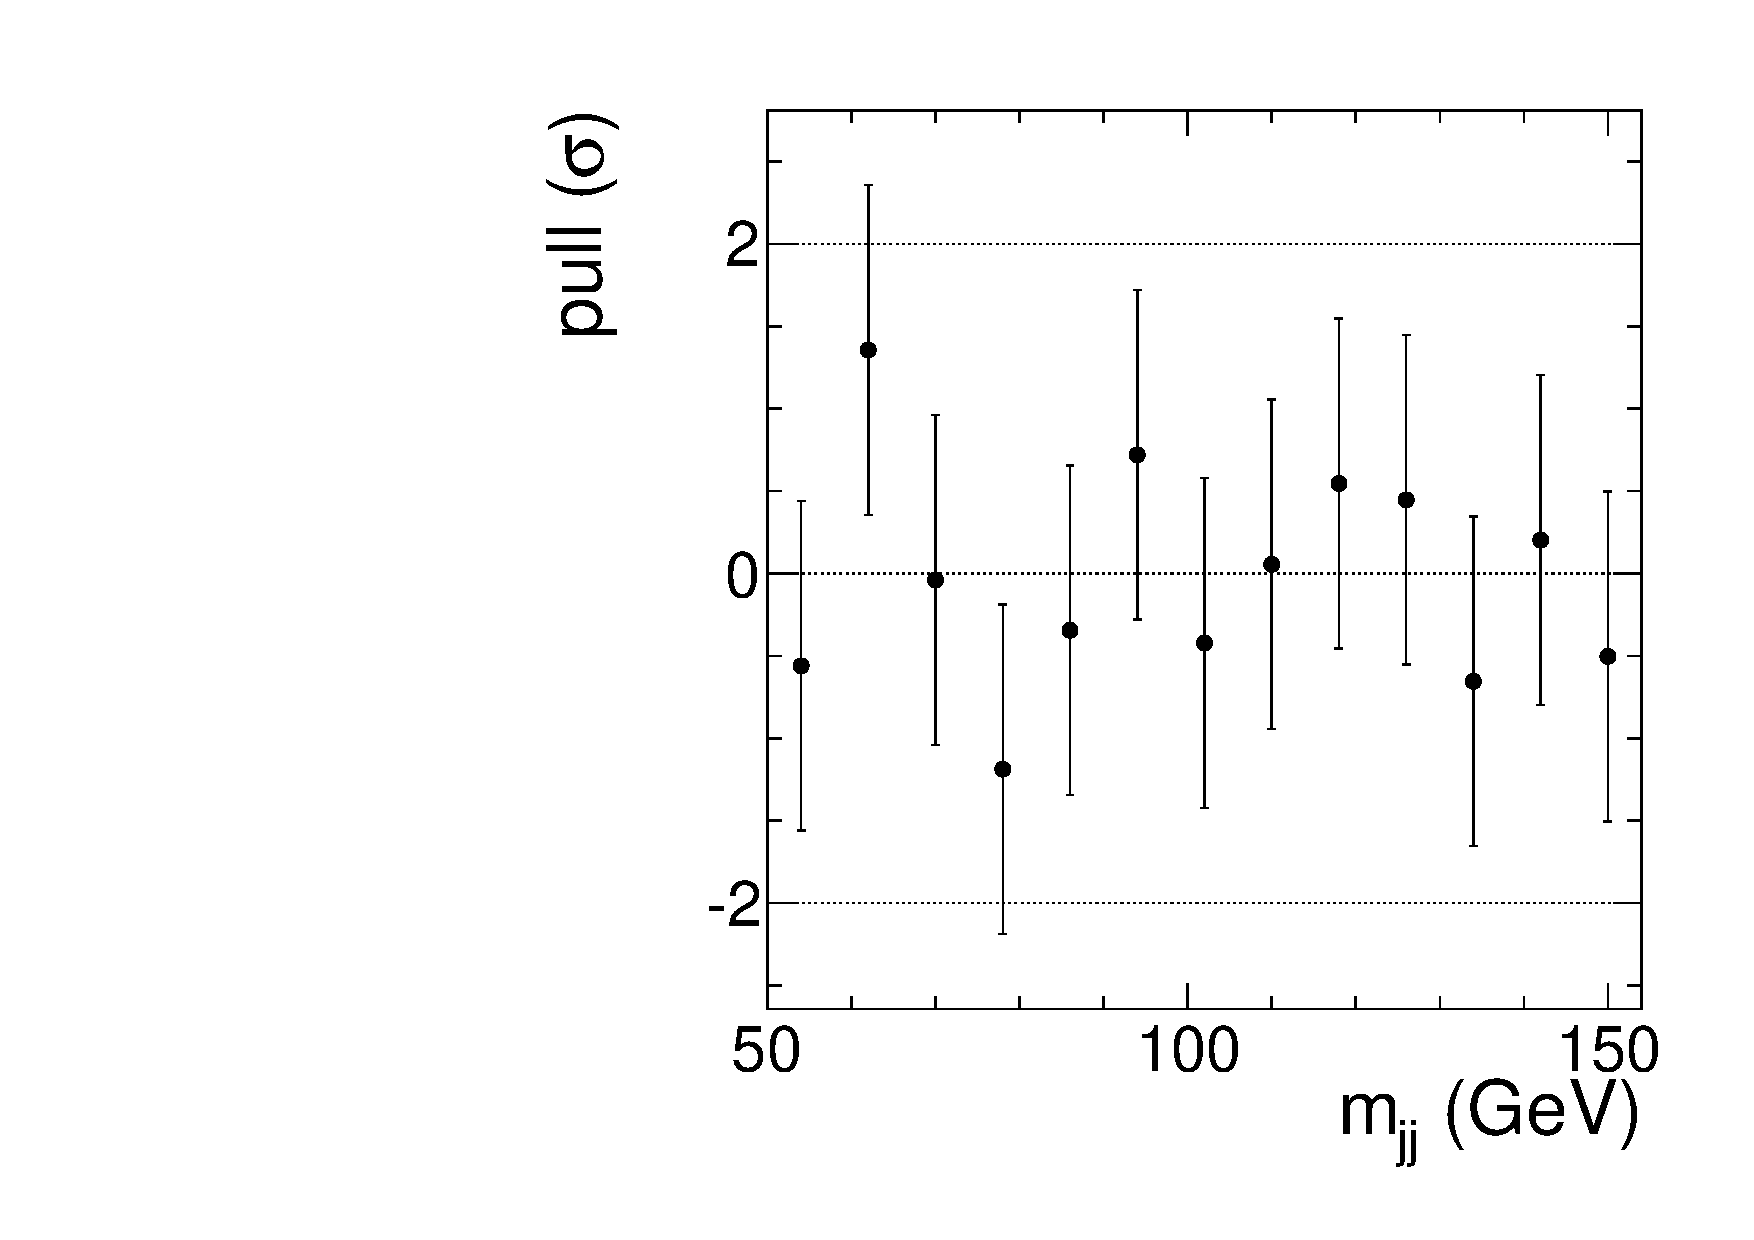
\includegraphics[width=0.49\textwidth]{plots/2012_FOURBSHAPES/HWW250lnujj_muon_mjj_pull}
  % \parbox[b][0.49\textwidth][r]{0.49\textwidth}{pull to be included when unblinded.}
  \caption{\label{fig:mjj_mH250}For the SM Higgs mass of 250~GeV, the
    distribution of the dijet invariant mass $m_{jj}$ is shown with
    muons on the left and electrons on the right.}
  % The pull
  %   distribution computed as [(Data - Fit)/ Fit uncertainty] is shown
  %   on the right. } %% The signal region is blinded.}
\end{figure}

\begin{figure}[!t]
  \centering
  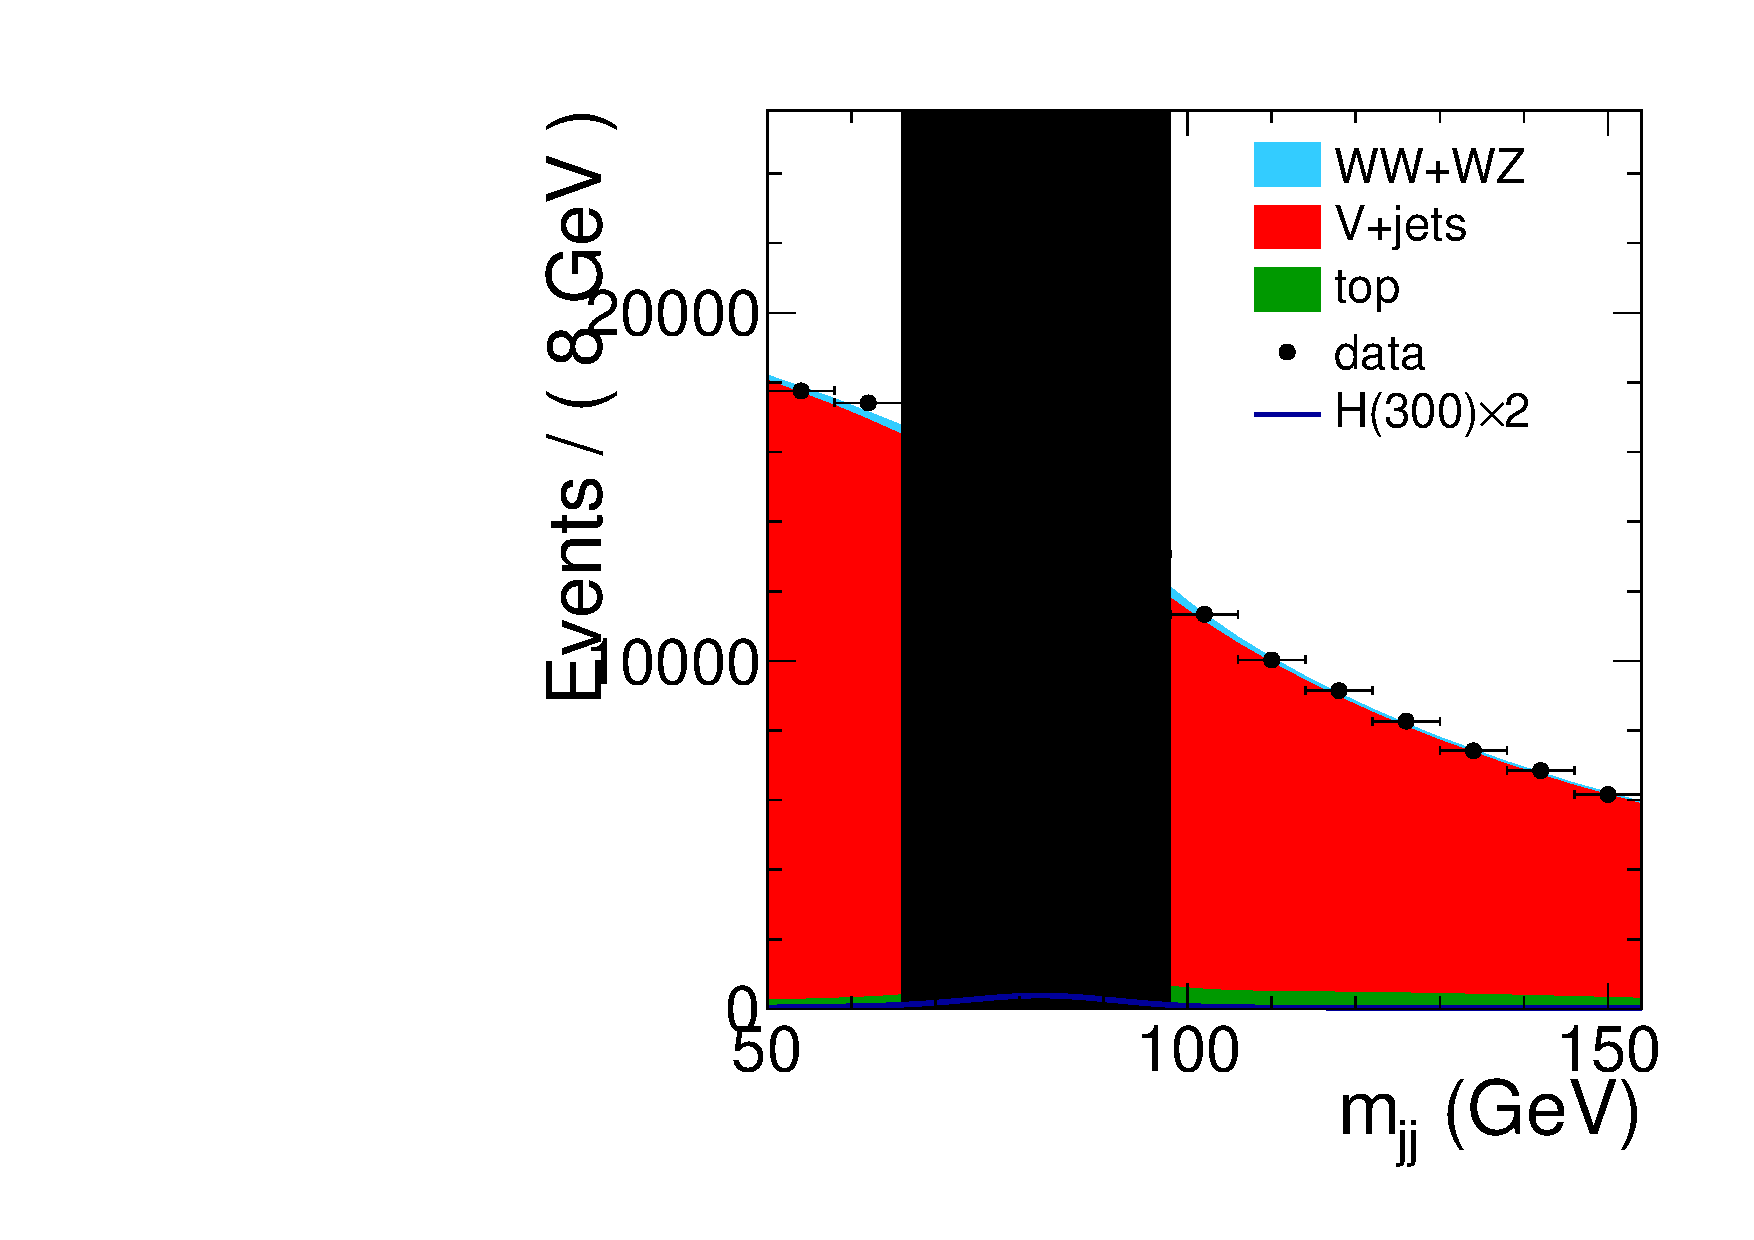
\includegraphics[width=0.49\textwidth]{plots/2012_FOURBSHAPES/HWW300lnujj_muon_mjj_stacked}
  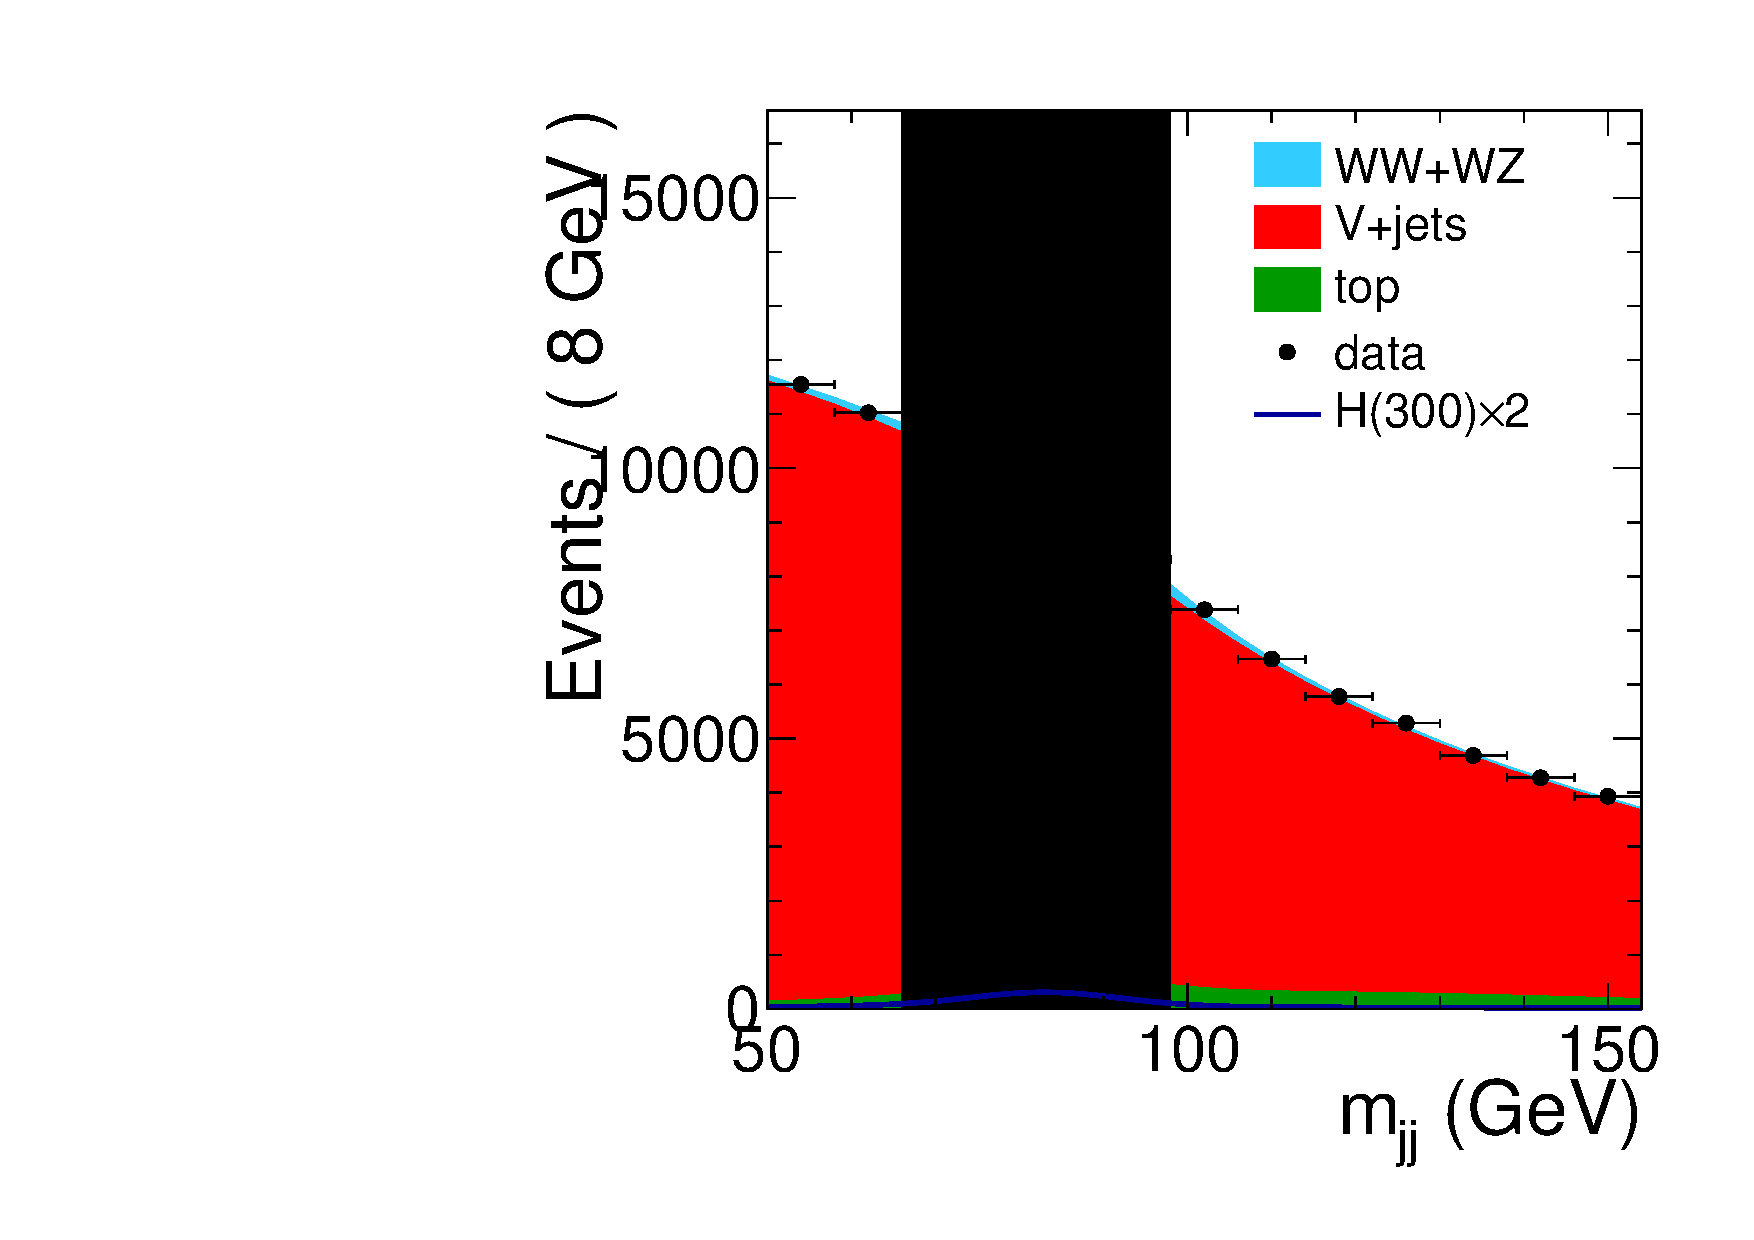
\includegraphics[width=0.49\textwidth]{plots/2012_FOURBSHAPES/HWW300lnujj_electron_mjj_stacked}
  %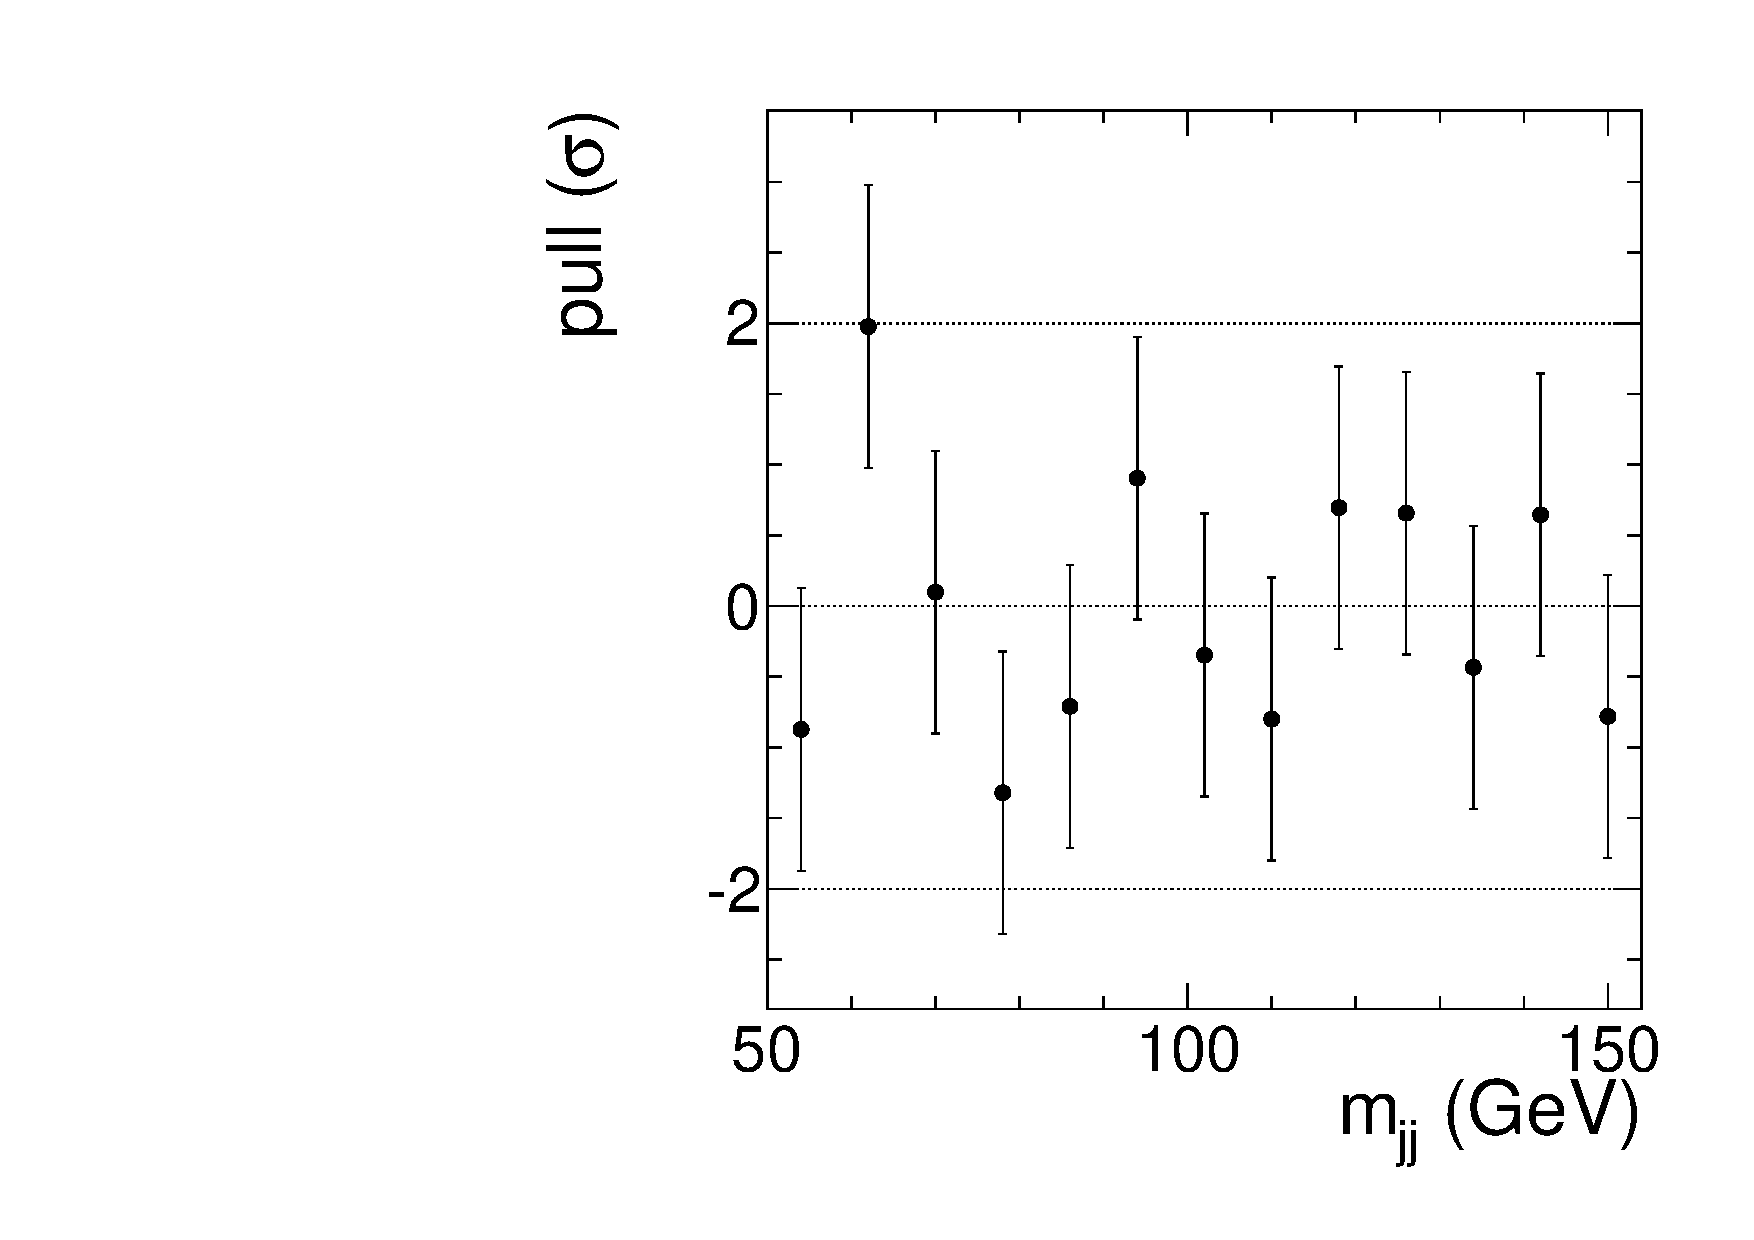
\includegraphics[width=0.49\textwidth]{plots/2012_FOURBSHAPES/HWW300lnujj_muon_mjj_pull}
  % \parbox[b][0.49\textwidth][r]{0.49\textwidth}{pull to be included when unblinded.}
  \caption{\label{fig:mjj_mH300}For the SM Higgs mass of 300~GeV, the
    distribution of the dijet invariant mass $m_{jj}$ is shown with
    muons on the left and electrons on the right.}
  % The pull
  %   distribution computed as [(Data - Fit)/ Fit uncertainty] is shown
  %   on the right. } %% The signal region is blinded.}
\end{figure}

\begin{figure}[!t]
  \centering
  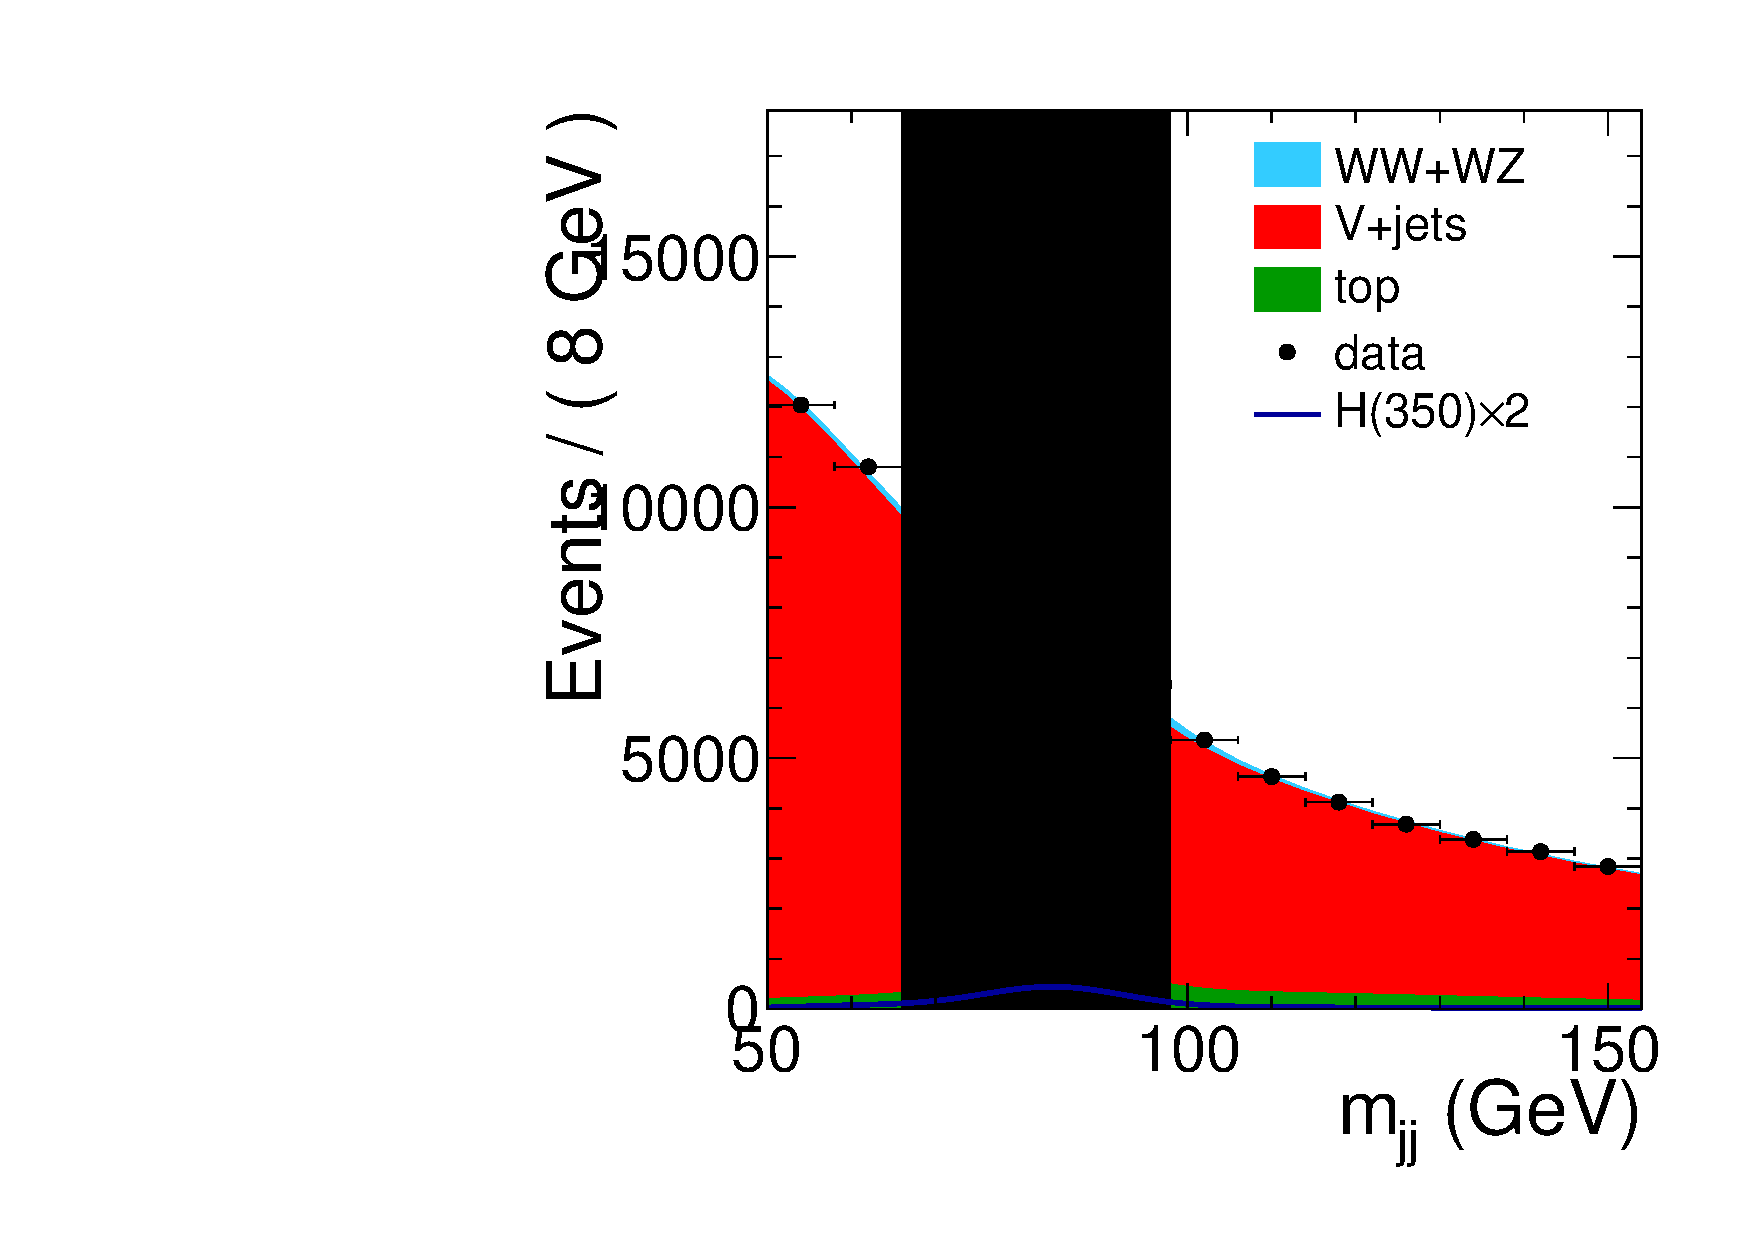
\includegraphics[width=0.49\textwidth]{plots/2012_FOURBSHAPES/HWW350lnujj_muon_mjj_stacked}
  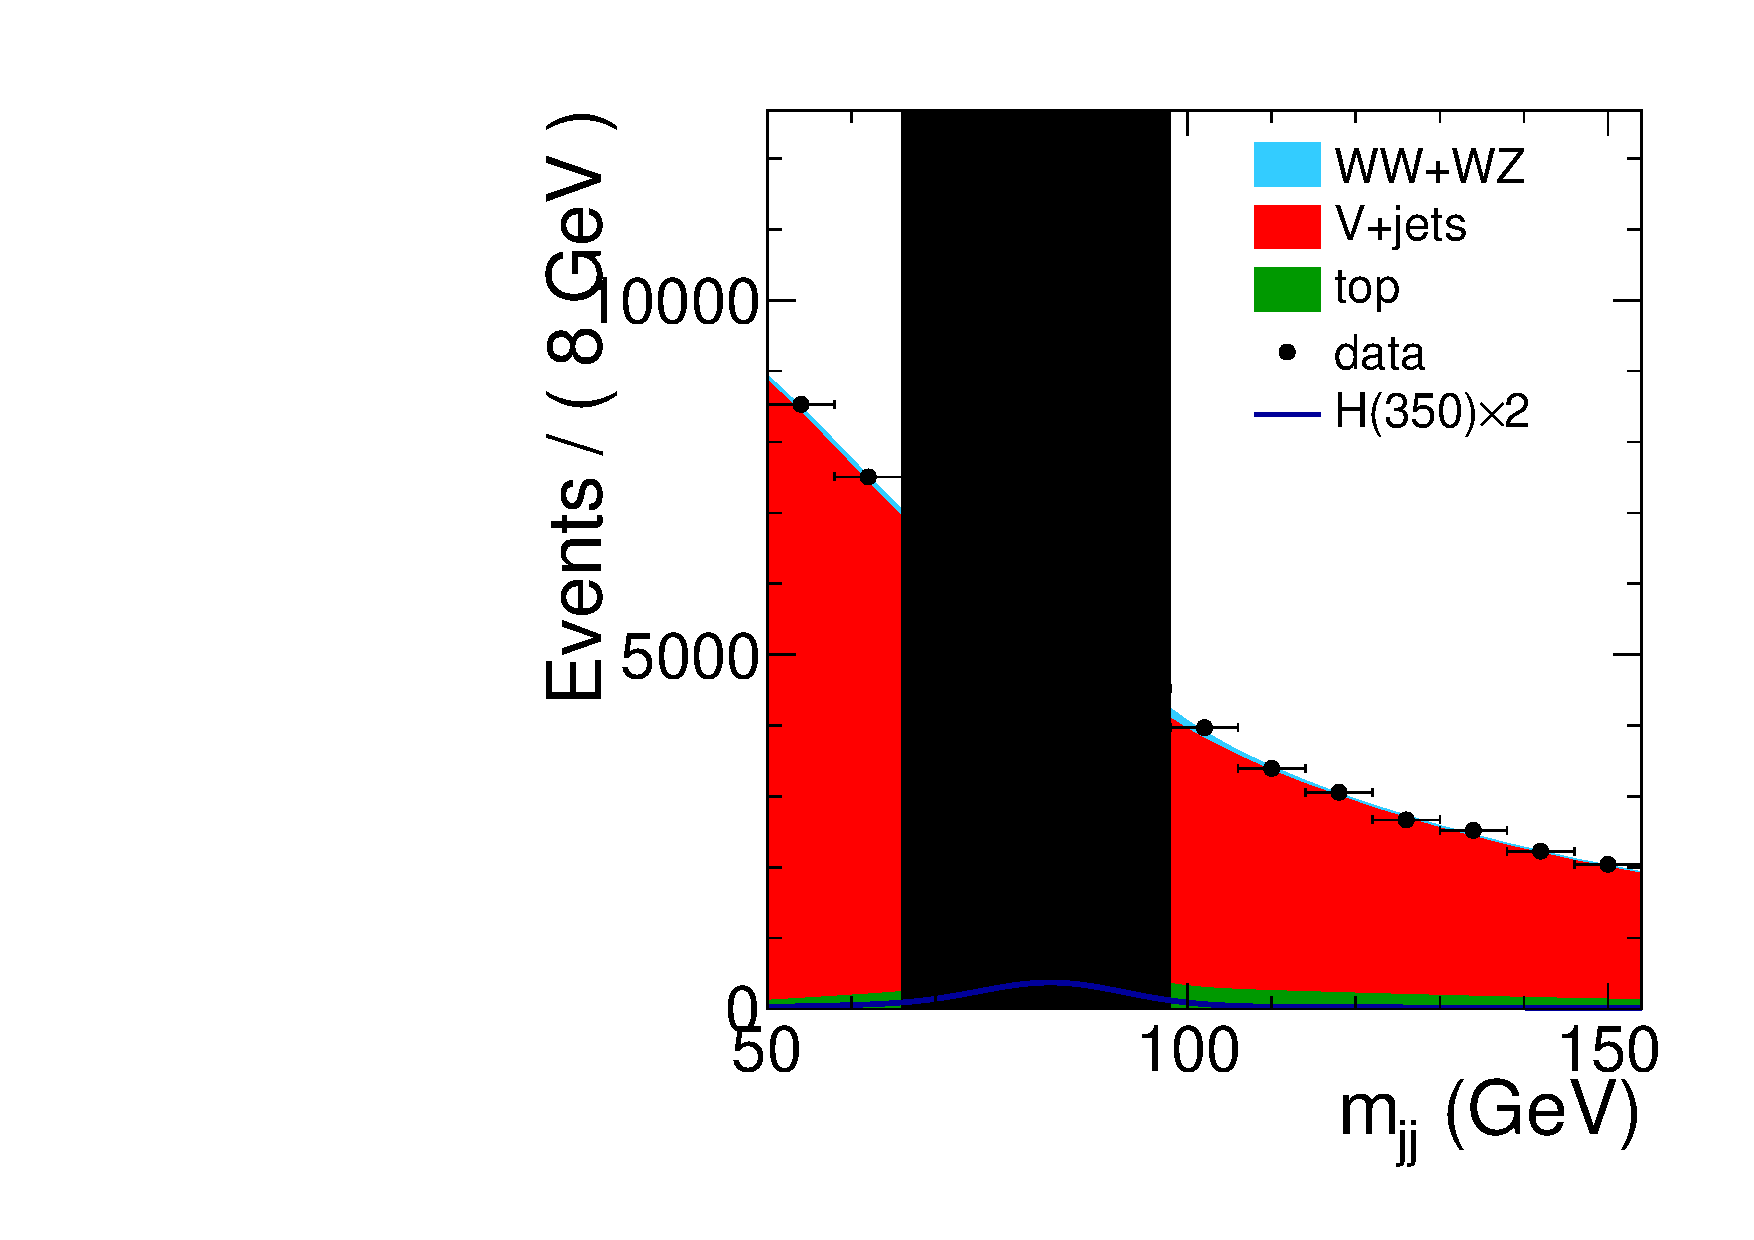
\includegraphics[width=0.49\textwidth]{plots/2012_FOURBSHAPES/HWW350lnujj_electron_mjj_stacked}
  %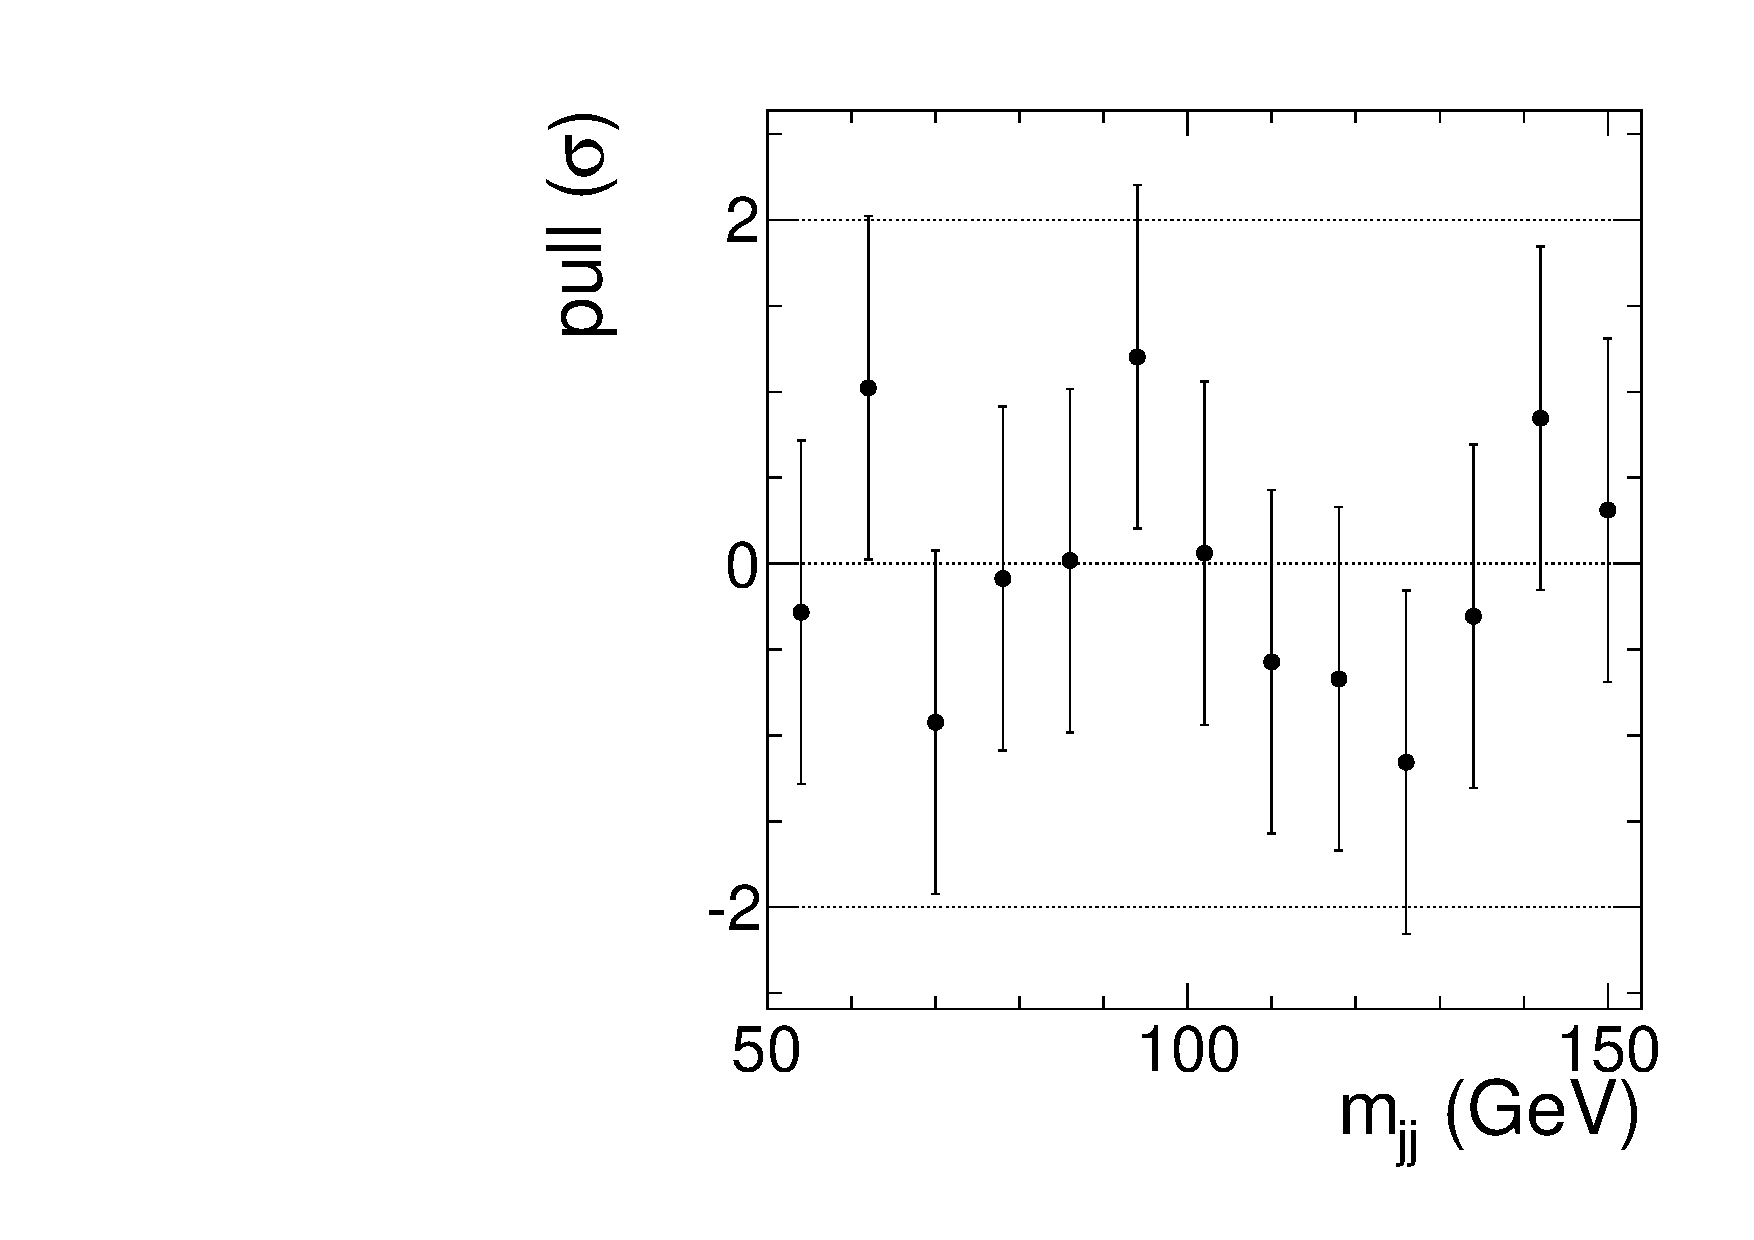
\includegraphics[width=0.49\textwidth]{plots/2012_FOURBSHAPES/HWW350lnujj_muon_mjj_pull}
  % \parbox[b][0.49\textwidth][r]{0.49\textwidth}{pull to be included when unblinded.}
  \caption{\label{fig:mjj_mH350}For the SM Higgs mass of 350~GeV, the
    distribution of the dijet invariant mass $m_{jj}$ is shown with
    muons on the left and electrons on the right.}
  % The pull
  %   distribution computed as [(Data - Fit)/ Fit uncertainty] is shown
  %   on the right. } %% The signal region is blinded.}
\end{figure}

\begin{figure}[!t]
  \centering
  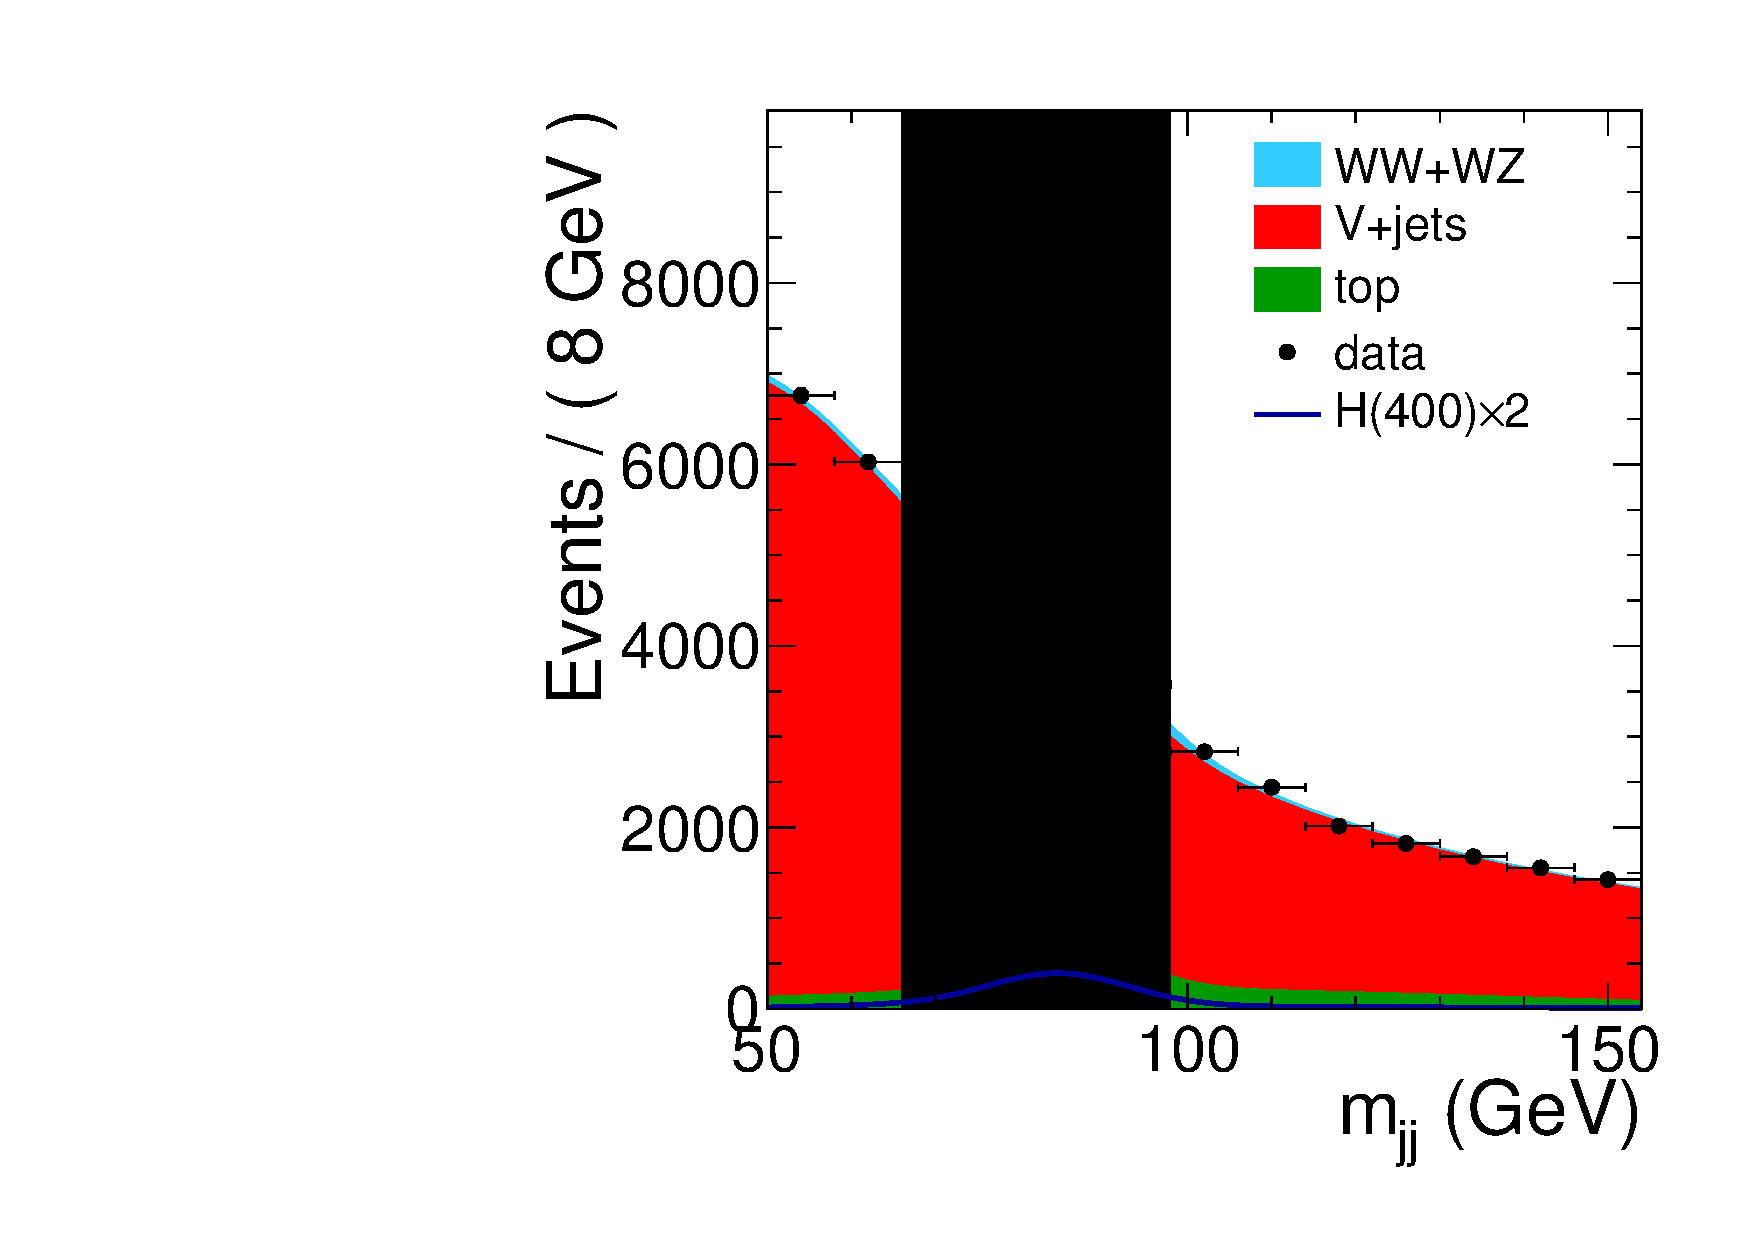
\includegraphics[width=0.49\textwidth]{plots/2012_FOURBSHAPES/HWW400lnujj_muon_mjj_stacked}
  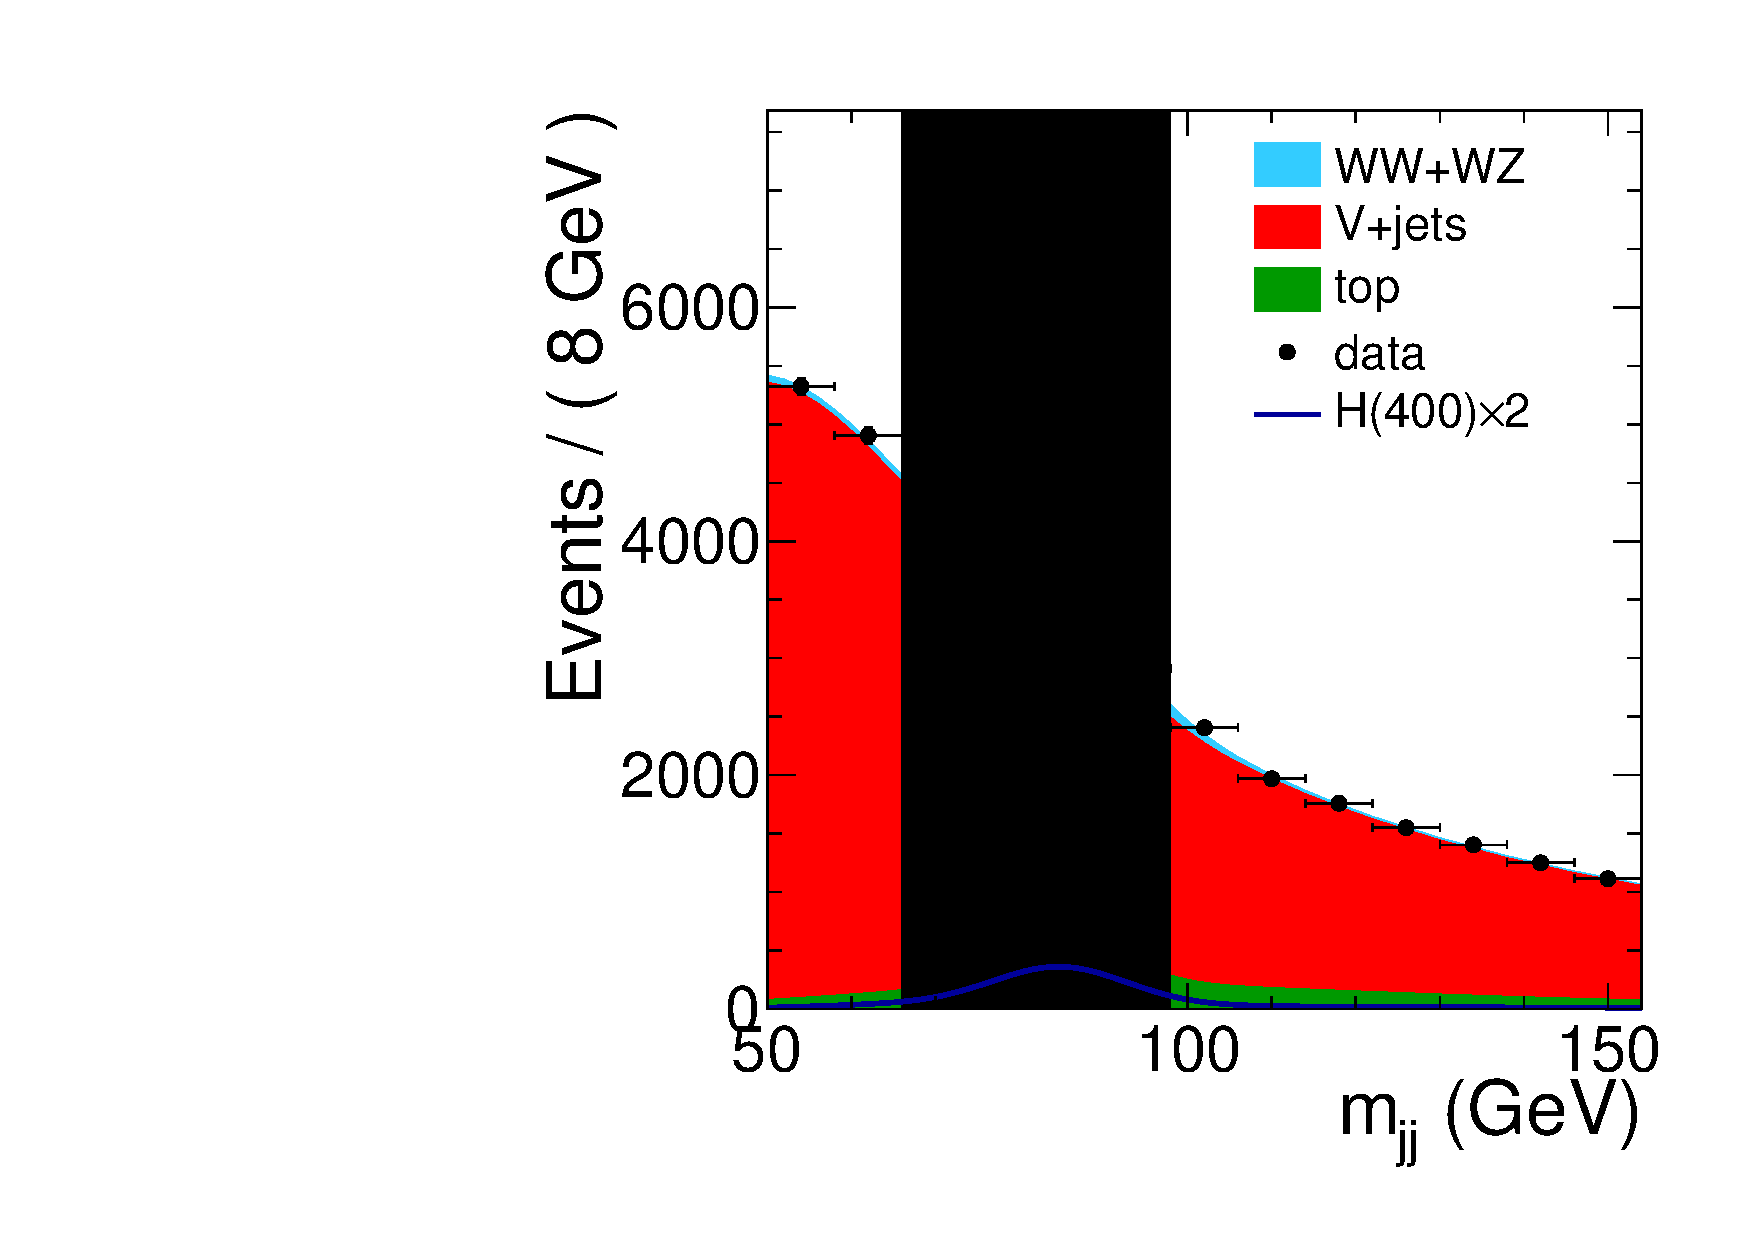
\includegraphics[width=0.49\textwidth]{plots/2012_FOURBSHAPES/HWW400lnujj_electron_mjj_stacked}
  %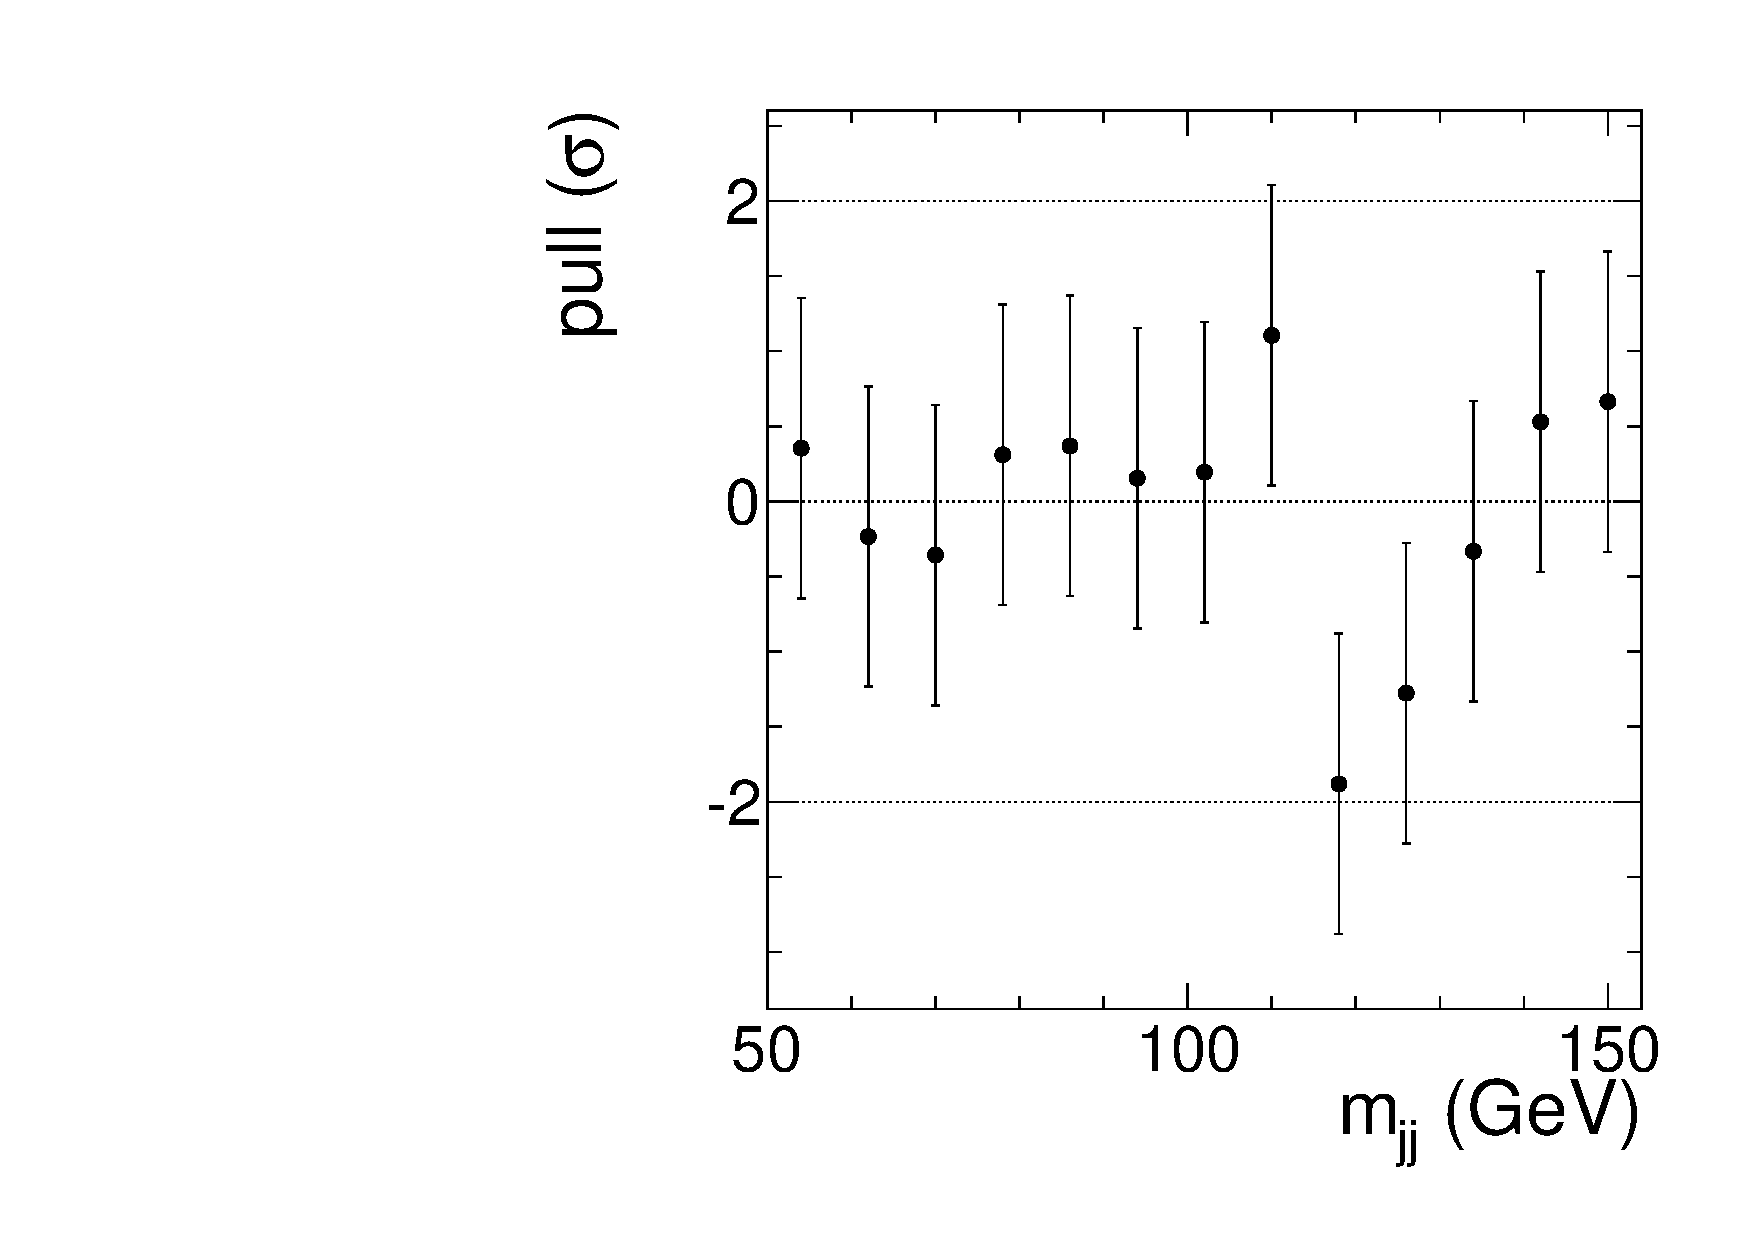
\includegraphics[width=0.49\textwidth]{plots/2012_FOURBSHAPES/HWW400lnujj_muon_mjj_pull}
  % \parbox[b][0.49\textwidth][r]{0.49\textwidth}{pull to be included when unblinded.}
  \caption{\label{fig:mjj_mH400}For the SM Higgs mass of 400~GeV, the
    distribution of the dijet invariant mass $m_{jj}$ is shown with
    muons on the left and electrons on the right.}
  % The pull
  %   distribution computed as [(Data - Fit)/ Fit uncertainty] is shown
  %   on the right. } %% The signal region is blinded.}
\end{figure}

\begin{figure}[!t]
  \centering
  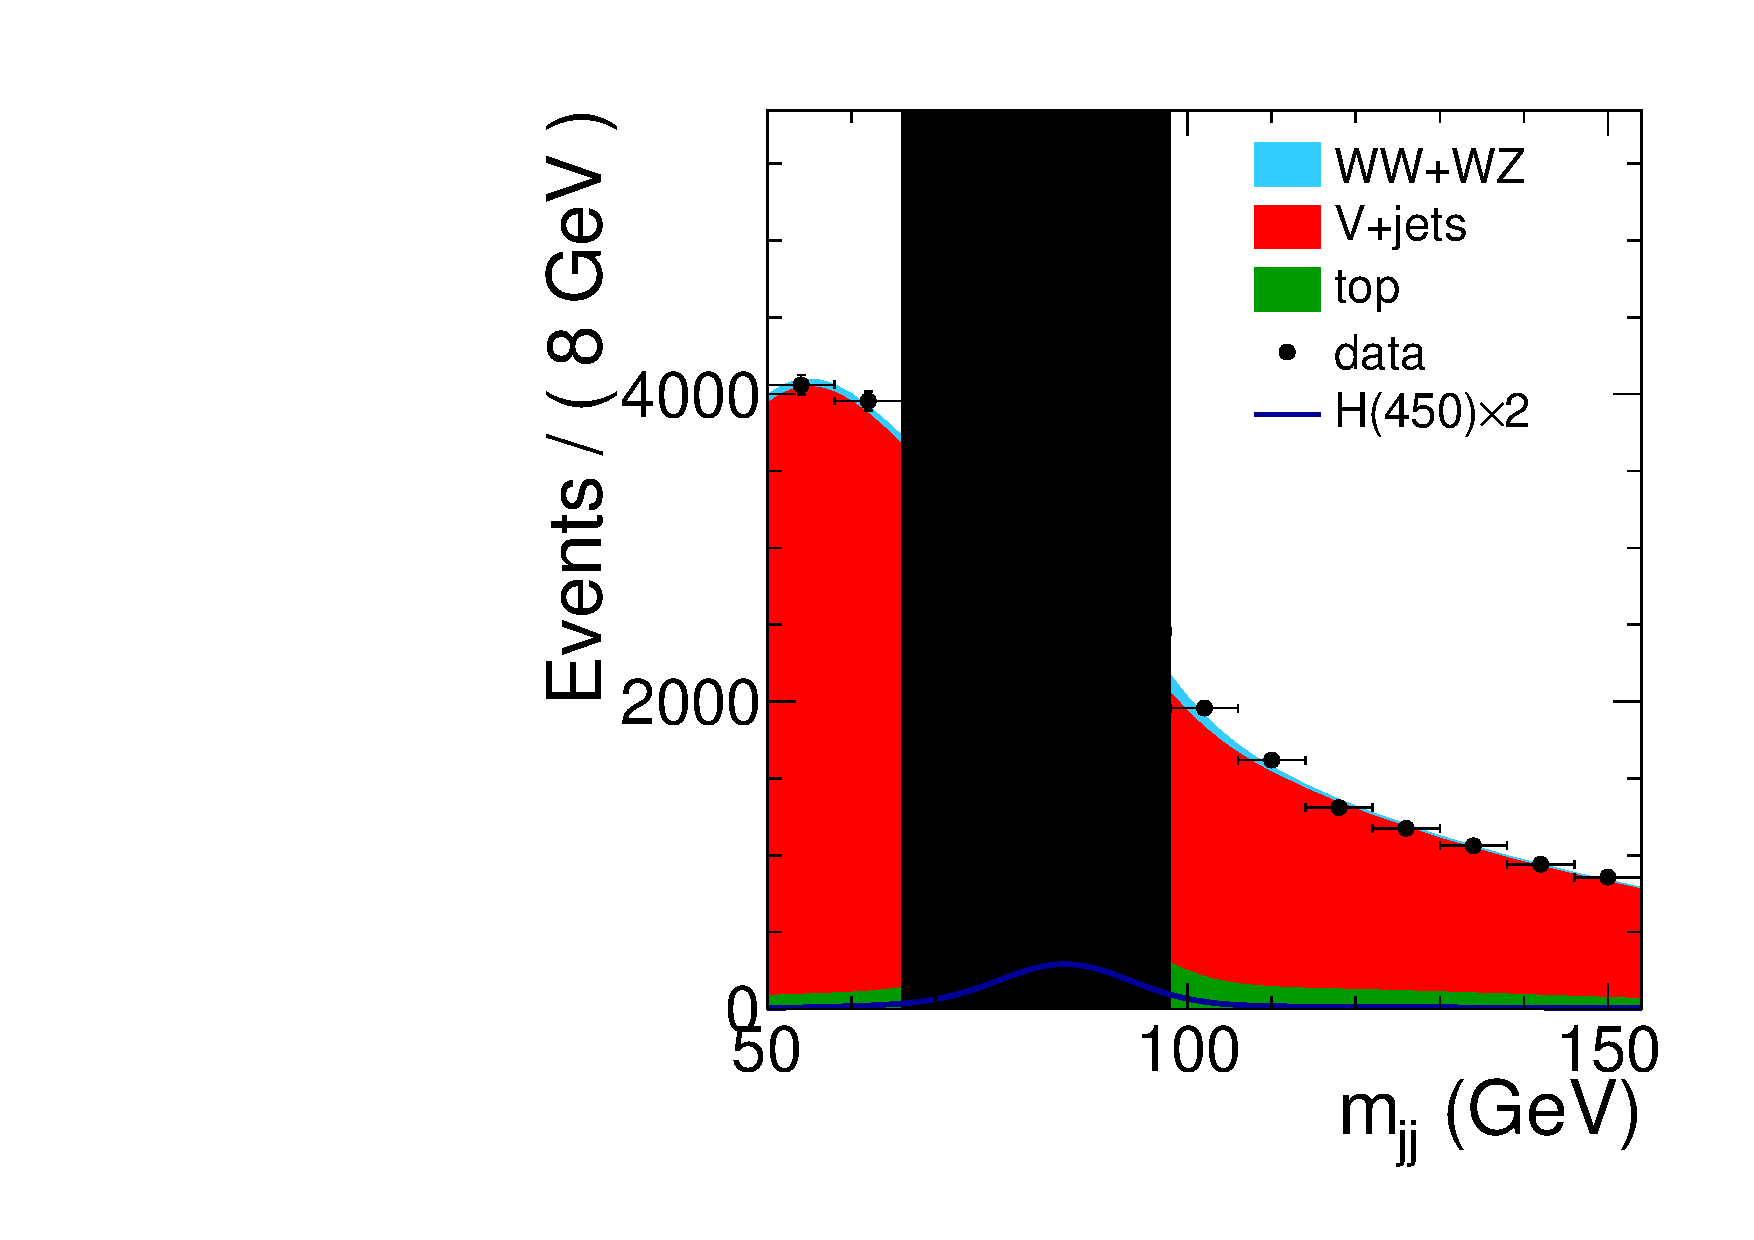
\includegraphics[width=0.49\textwidth]{plots/2012_FOURBSHAPES/HWW450lnujj_muon_mjj_stacked}
  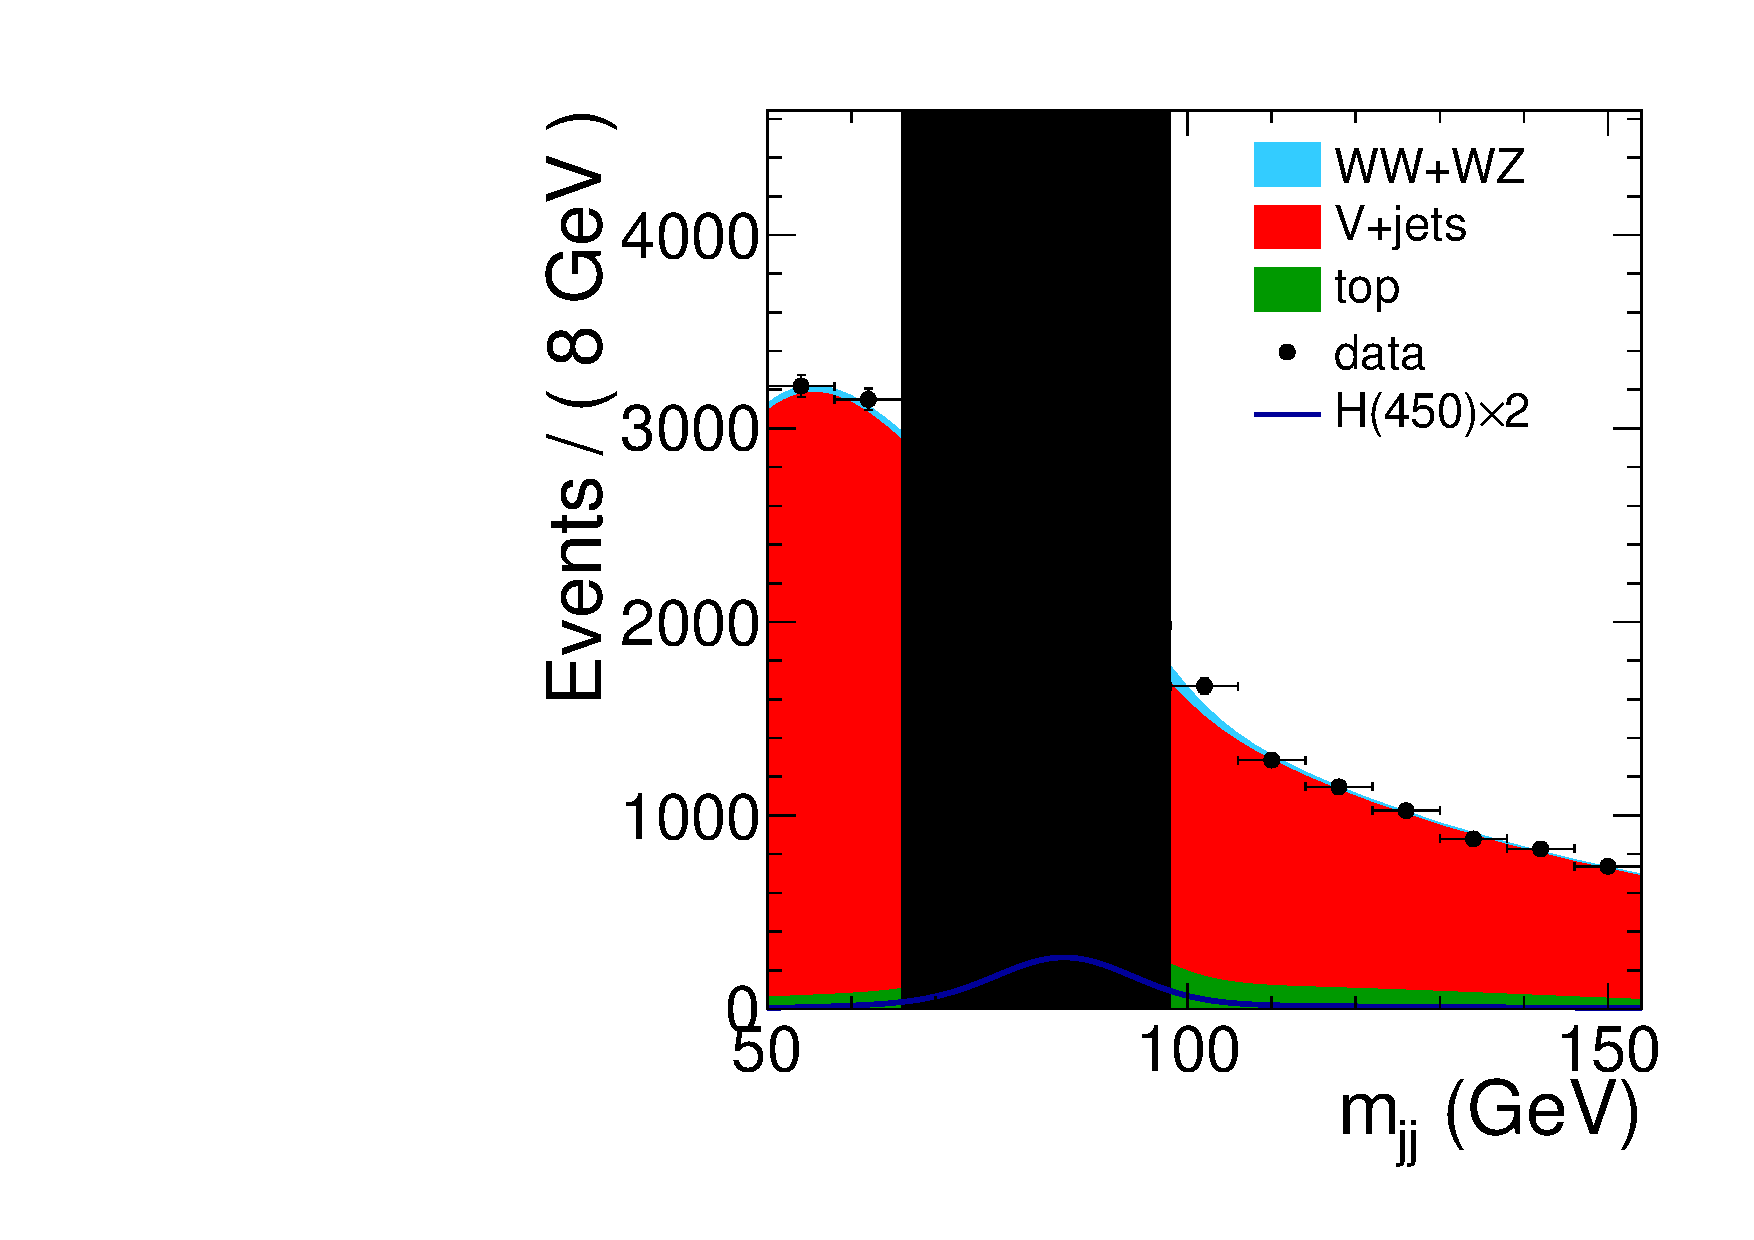
\includegraphics[width=0.49\textwidth]{plots/2012_FOURBSHAPES/HWW450lnujj_electron_mjj_stacked}
  %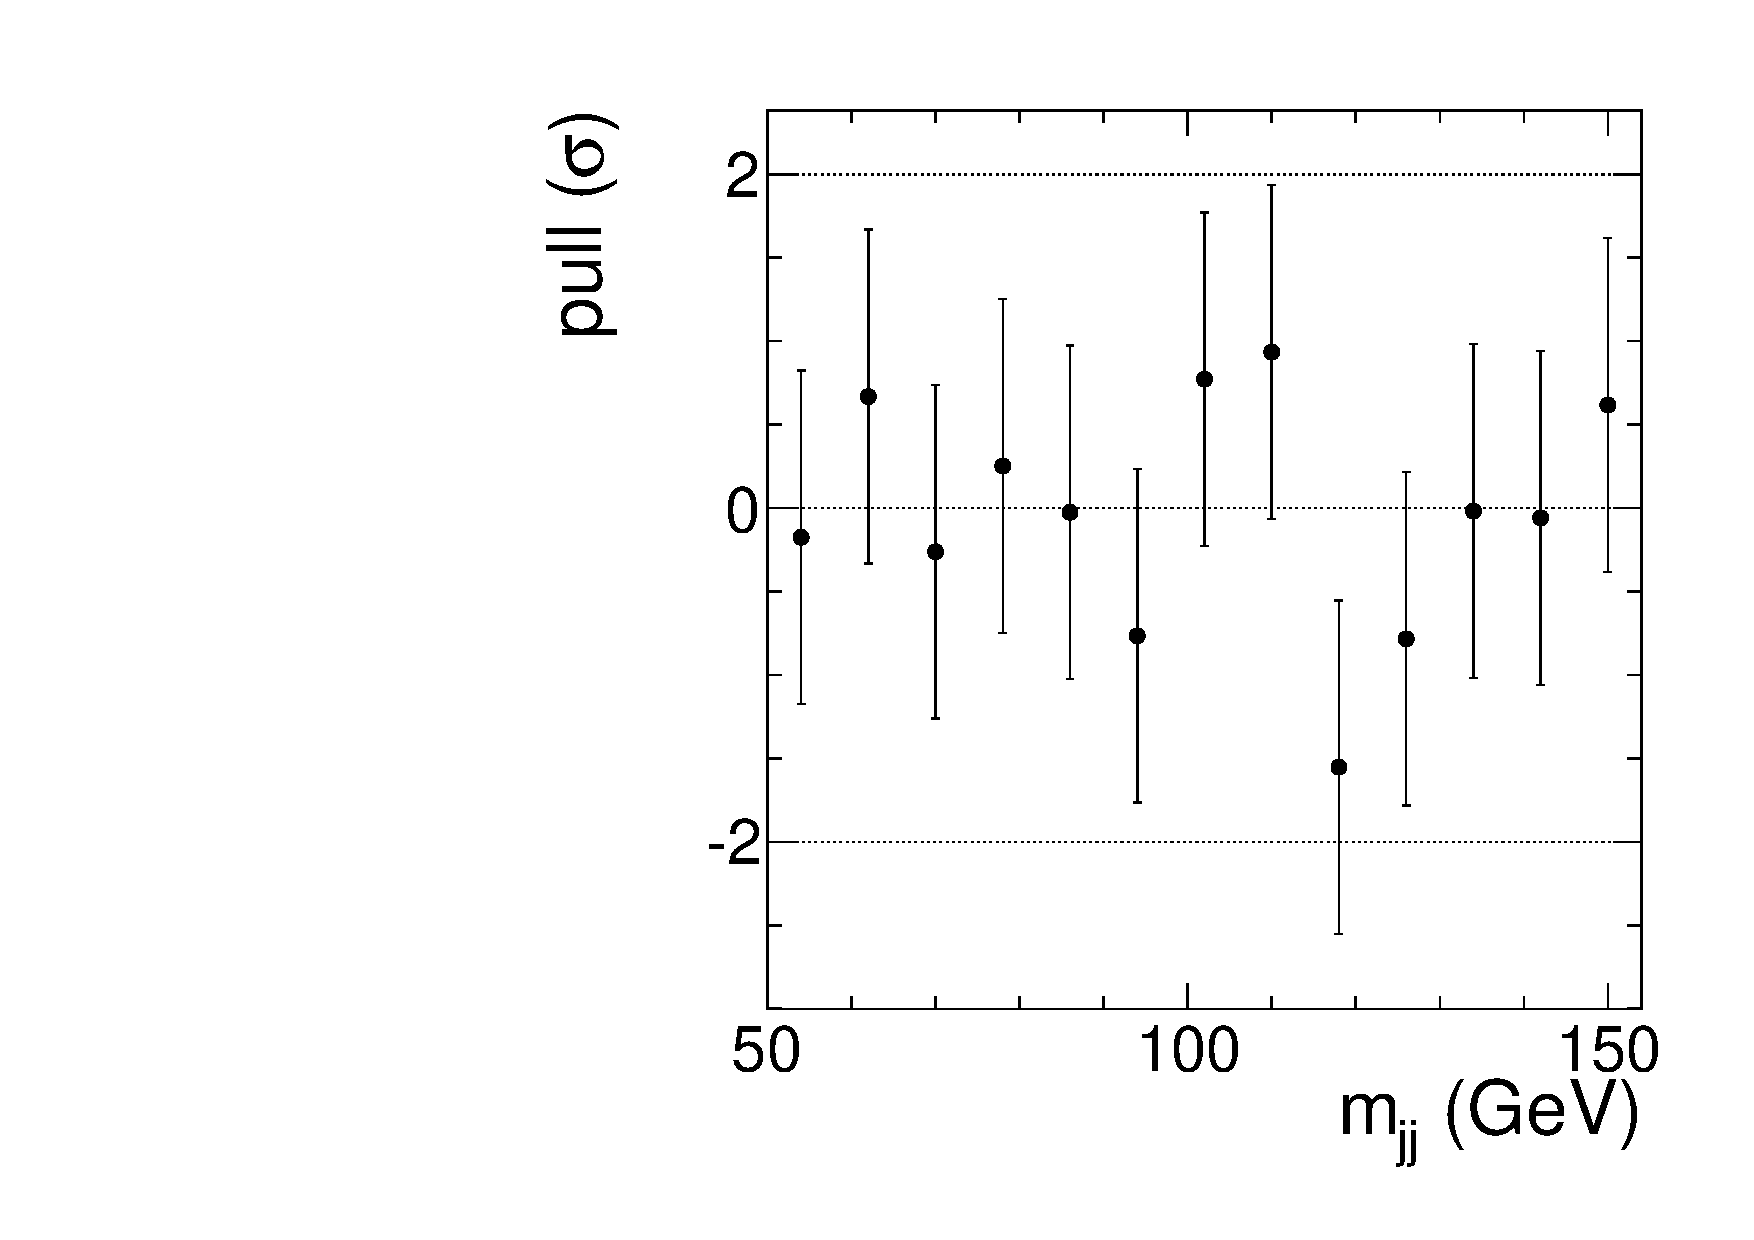
\includegraphics[width=0.49\textwidth]{plots/2012_FOURBSHAPES/HWW450lnujj_muon_mjj_pull}
  % \parbox[b][0.49\textwidth][r]{0.49\textwidth}{pull to be included when unblinded.}
  \caption{\label{fig:mjj_mH450}For the SM Higgs mass of 450~GeV, the
    distribution of the dijet invariant mass $m_{jj}$ is shown with
    muons on the left and electrons on the right.}
  % The pull
  %   distribution computed as [(Data - Fit)/ Fit uncertainty] is shown
  %   on the right. } %% The signal region is blinded.}
\end{figure}

\begin{figure}[!t]
  \centering
  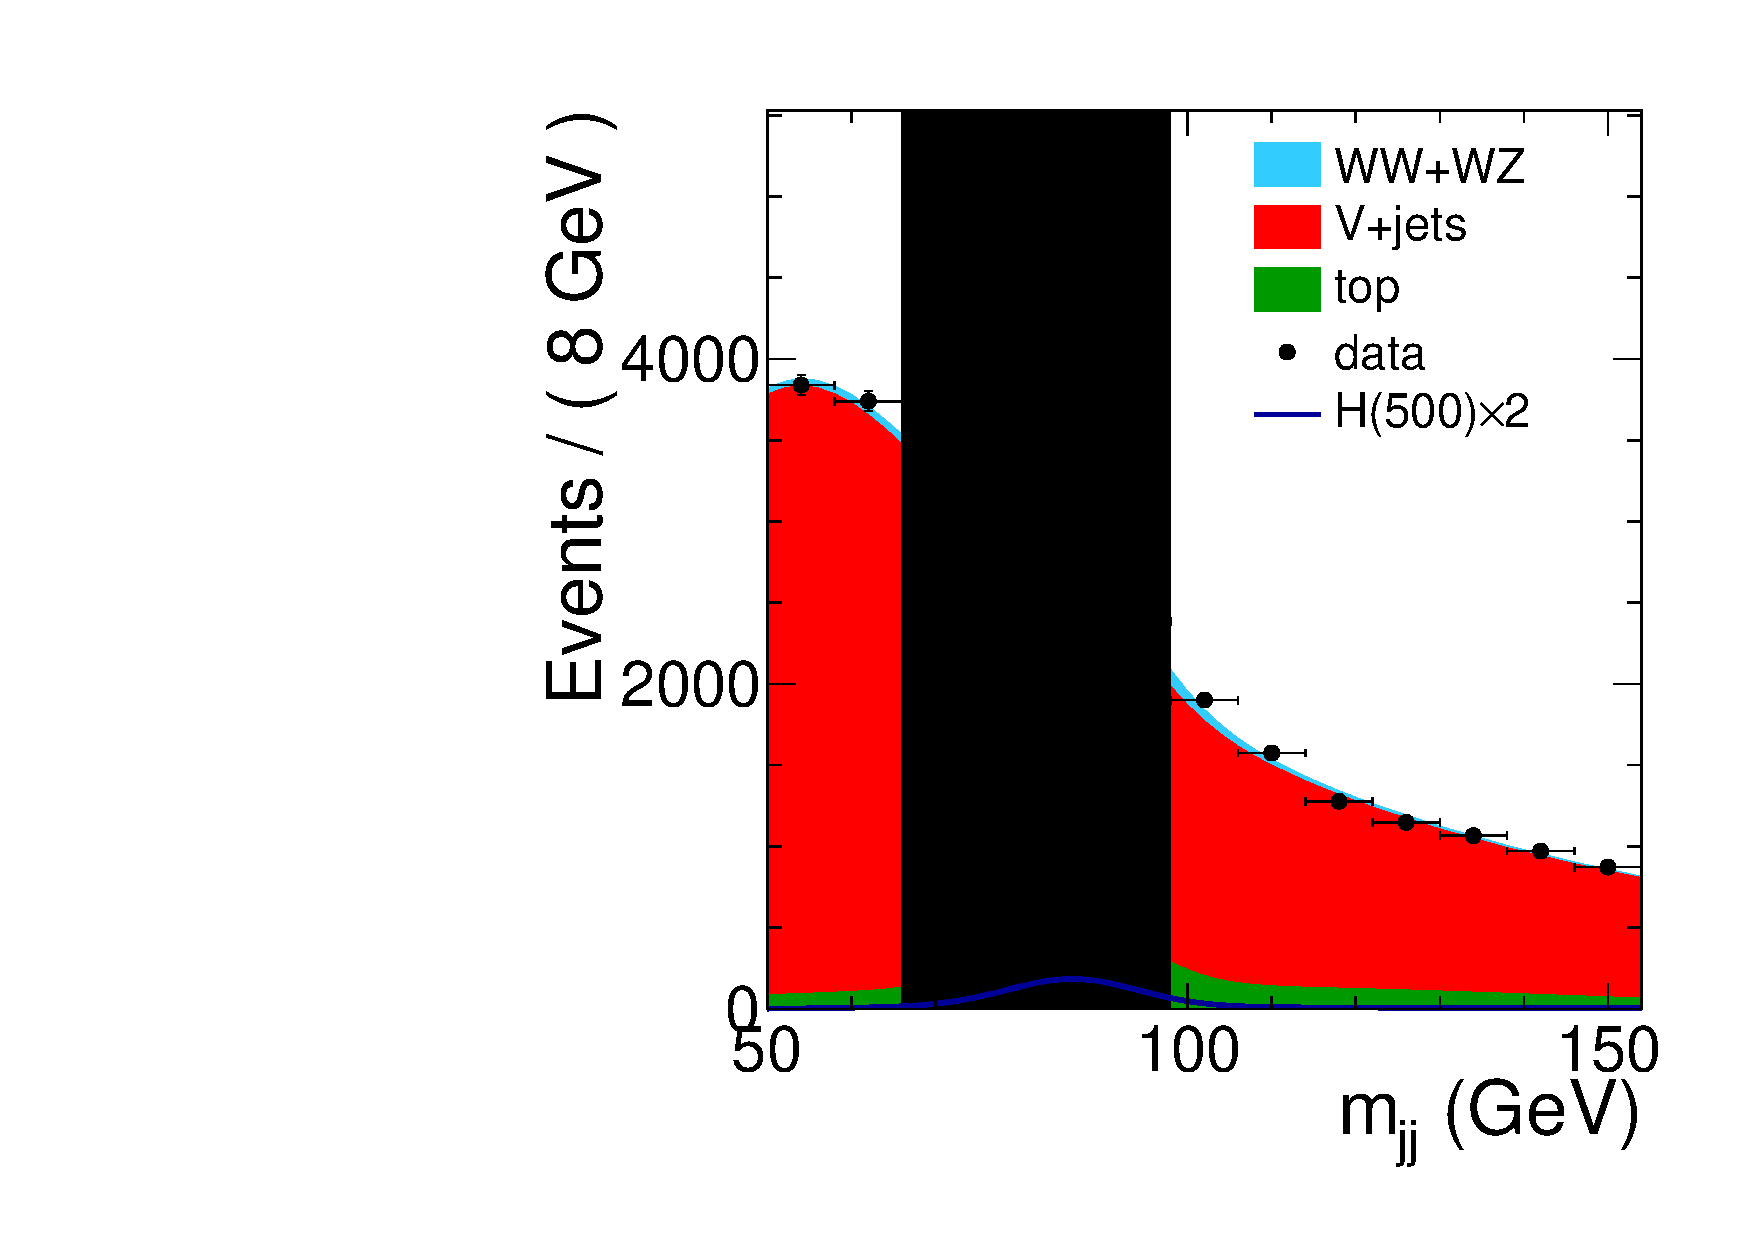
\includegraphics[width=0.49\textwidth]{plots/2012_FOURBSHAPES/HWW500lnujj_muon_mjj_stacked}
  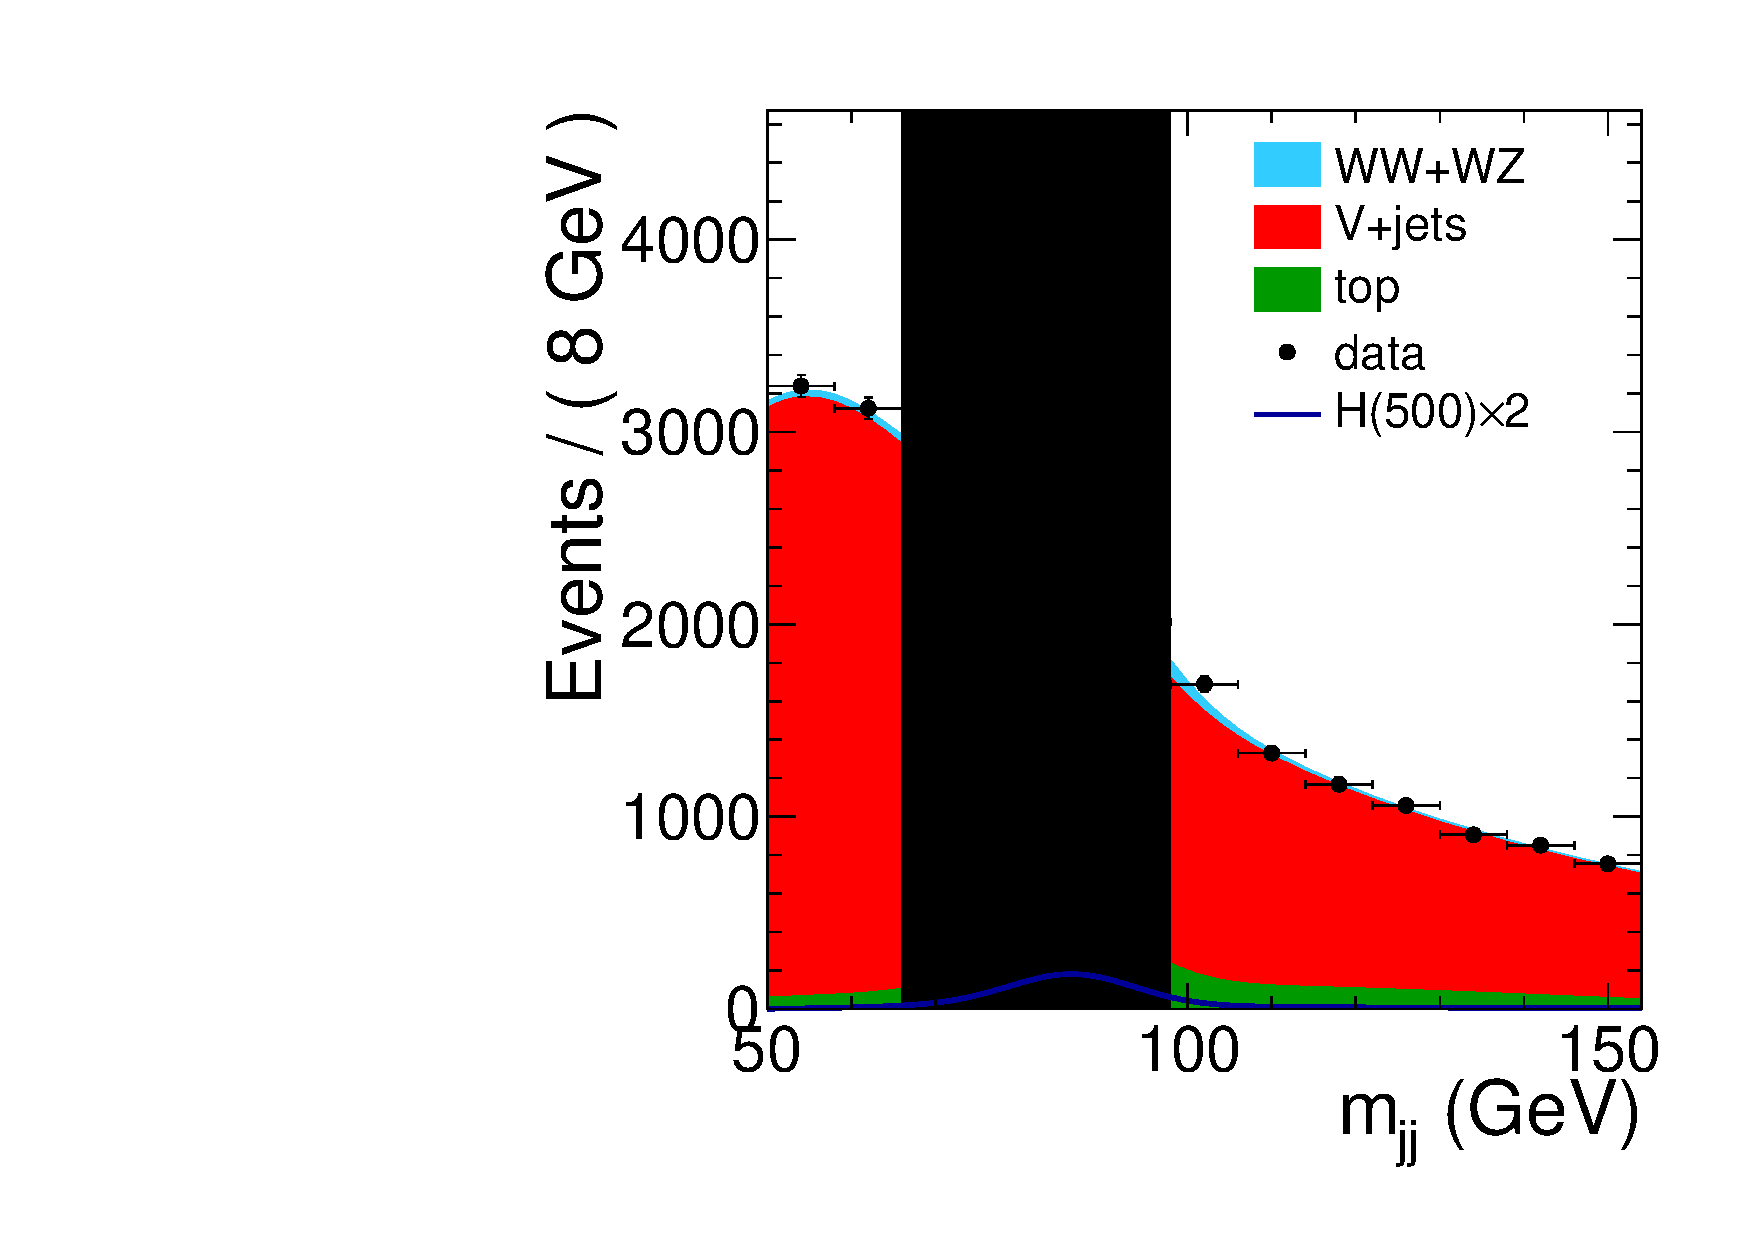
\includegraphics[width=0.49\textwidth]{plots/2012_FOURBSHAPES/HWW500lnujj_electron_mjj_stacked}
  %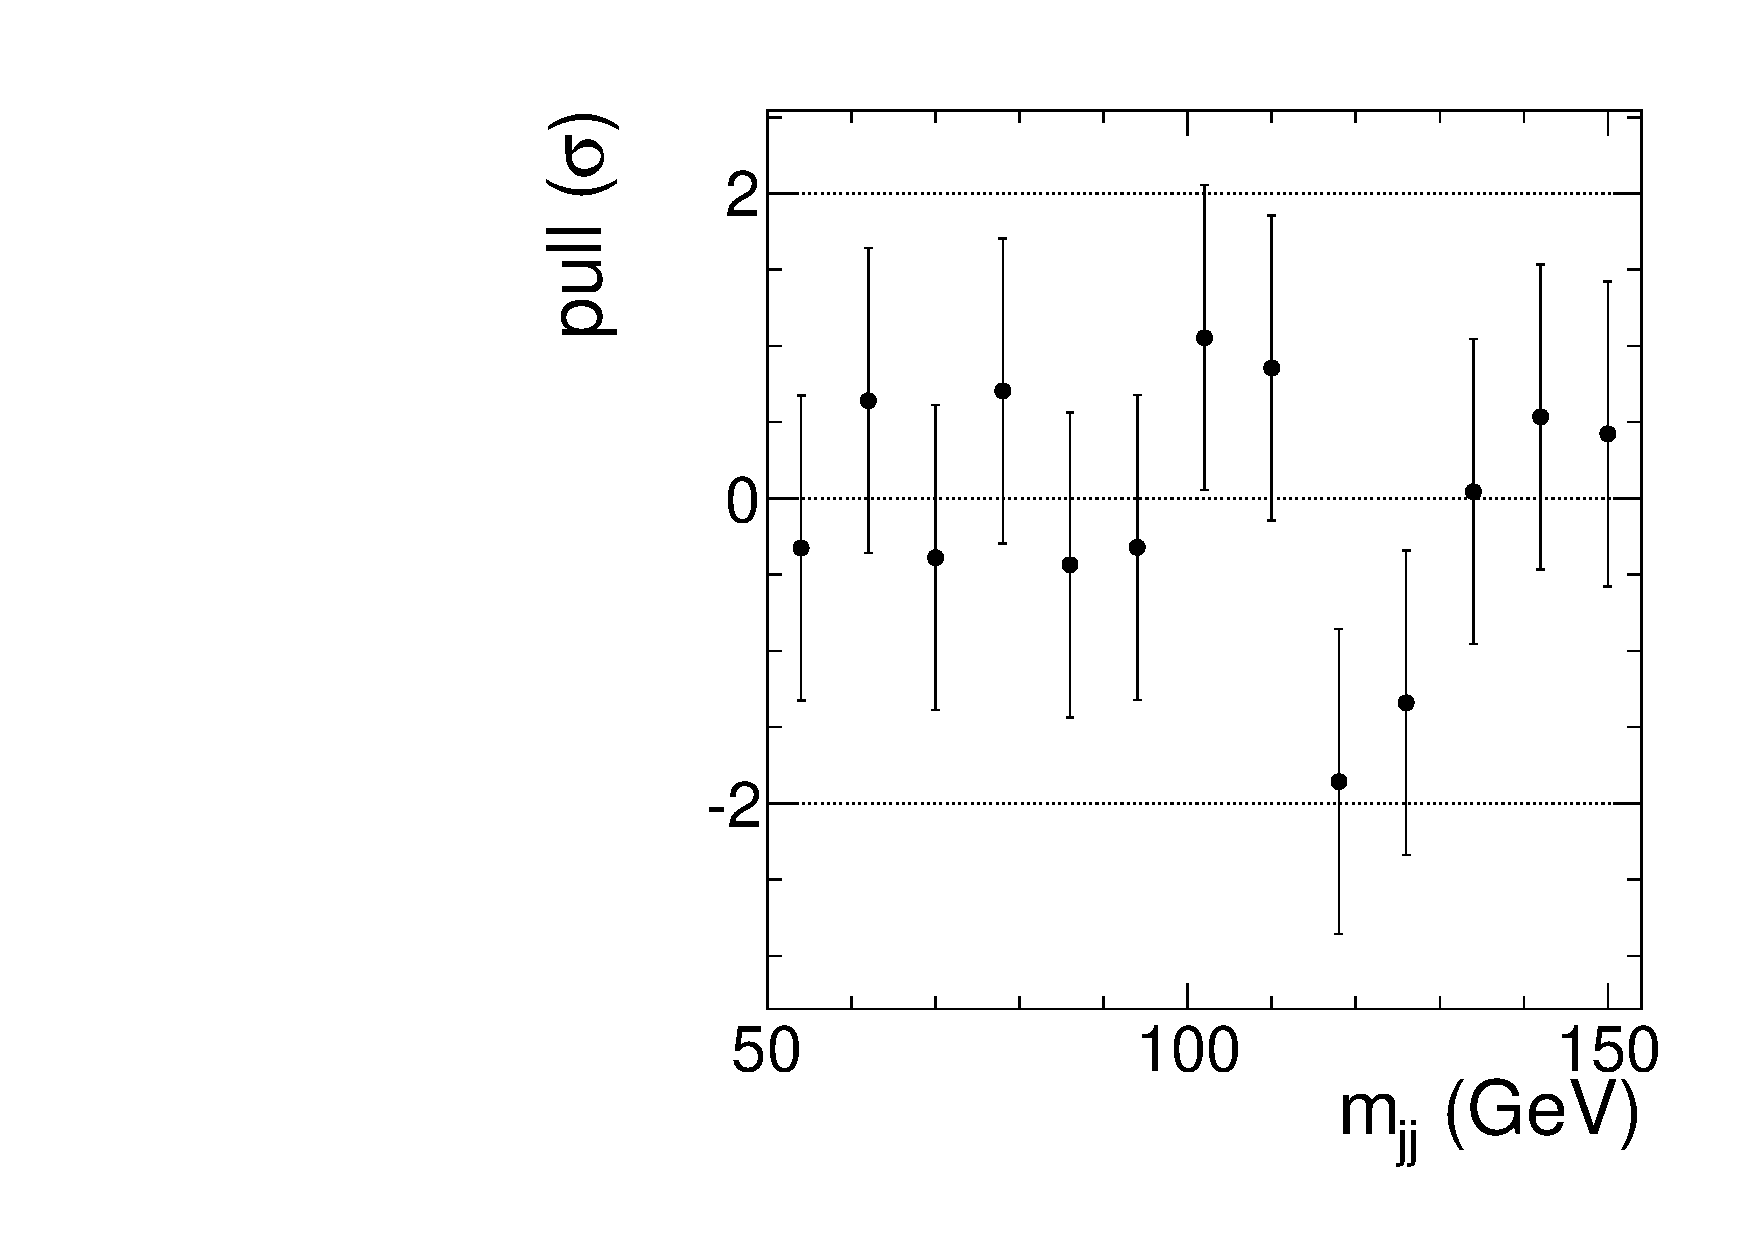
\includegraphics[width=0.49\textwidth]{plots/2012_FOURBSHAPES/HWW500lnujj_muon_mjj_pull}
  % \parbox[b][0.49\textwidth][r]{0.49\textwidth}{pull to be included when unblinded.}
  \caption{\label{fig:mjj_mH500}For the SM Higgs mass of 500~GeV, the
    distribution of the dijet invariant mass $m_{jj}$ is shown with
    muons on the left and electrons on the right.}
  % The pull
  %   distribution computed as [(Data - Fit)/ Fit uncertainty] is shown
  %   on the right. } %% The signal region is blinded.}
\end{figure}

\begin{figure}[!t]
  \centering
  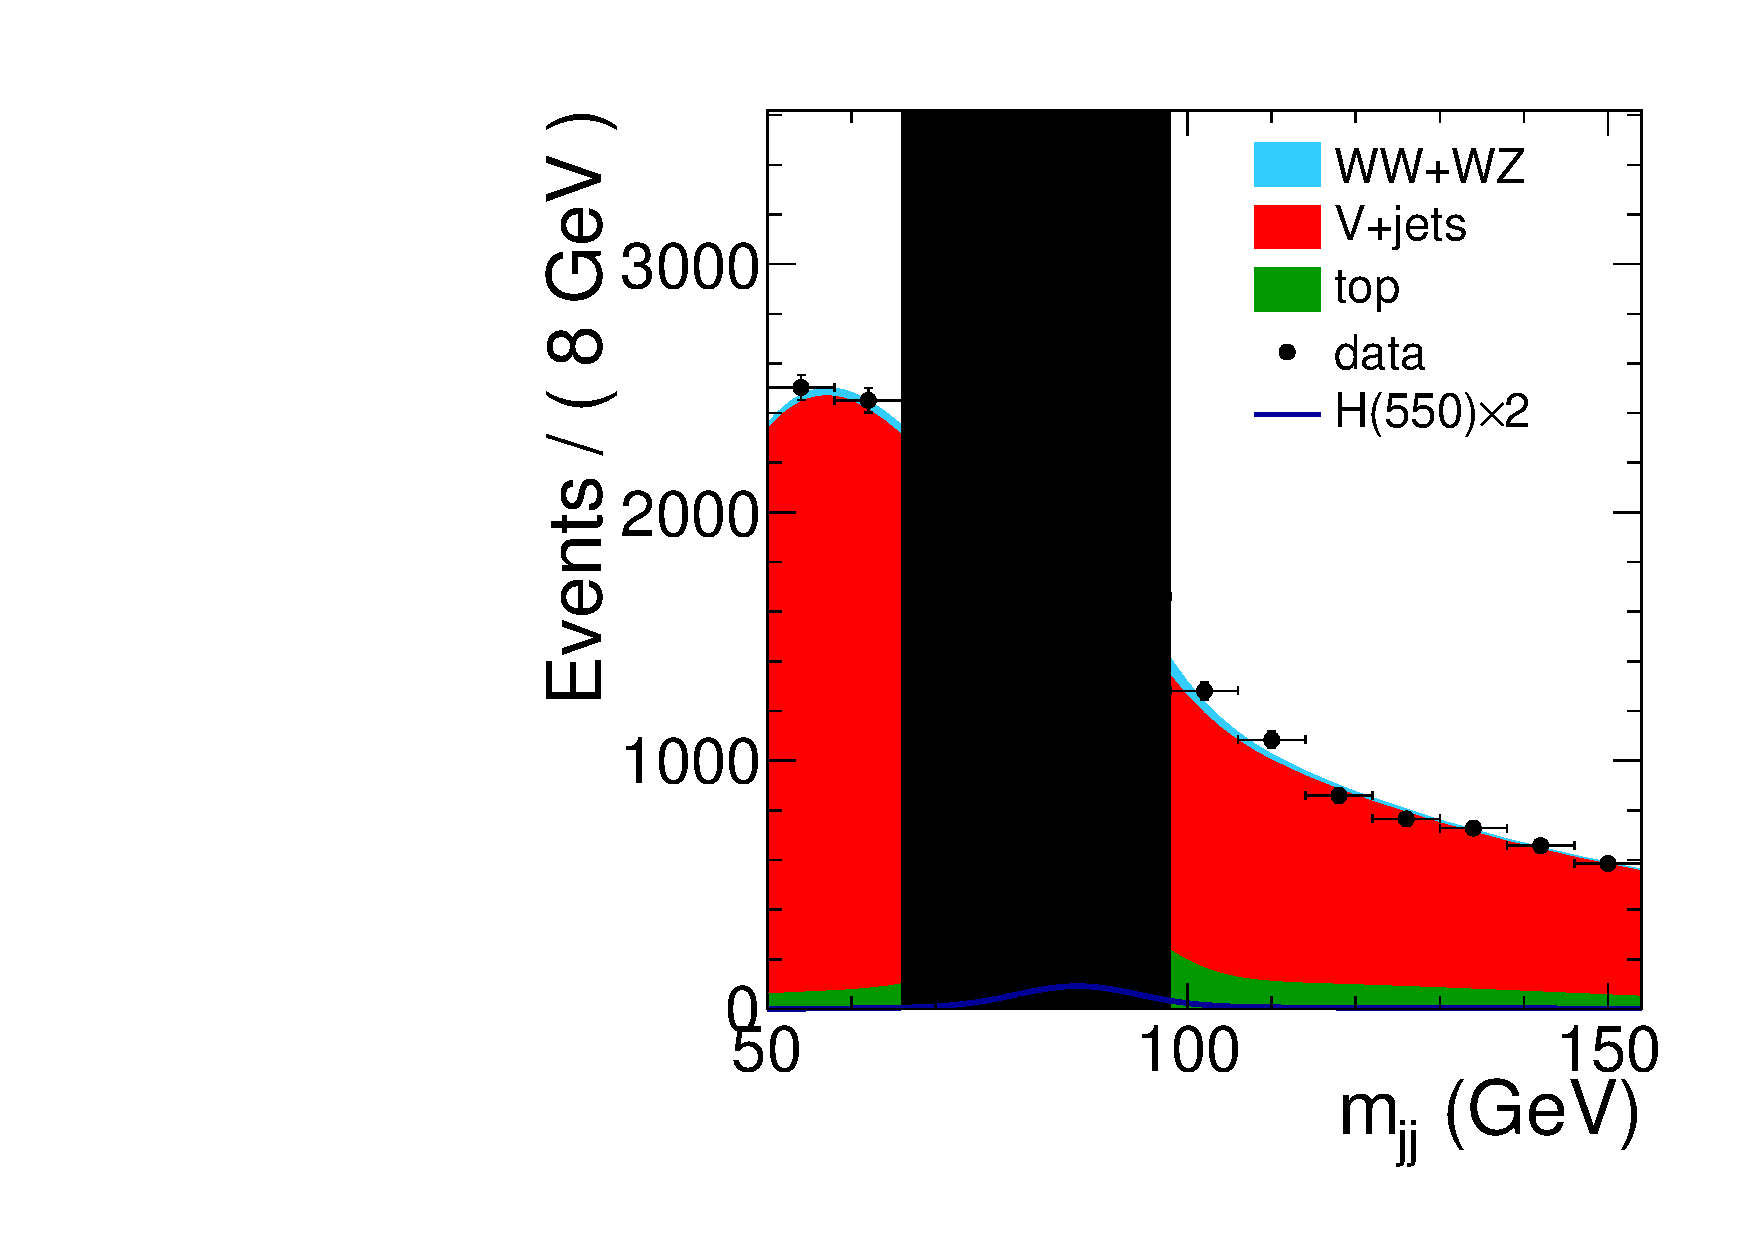
\includegraphics[width=0.49\textwidth]{plots/2012_FOURBSHAPES/HWW550lnujj_muon_mjj_stacked}
  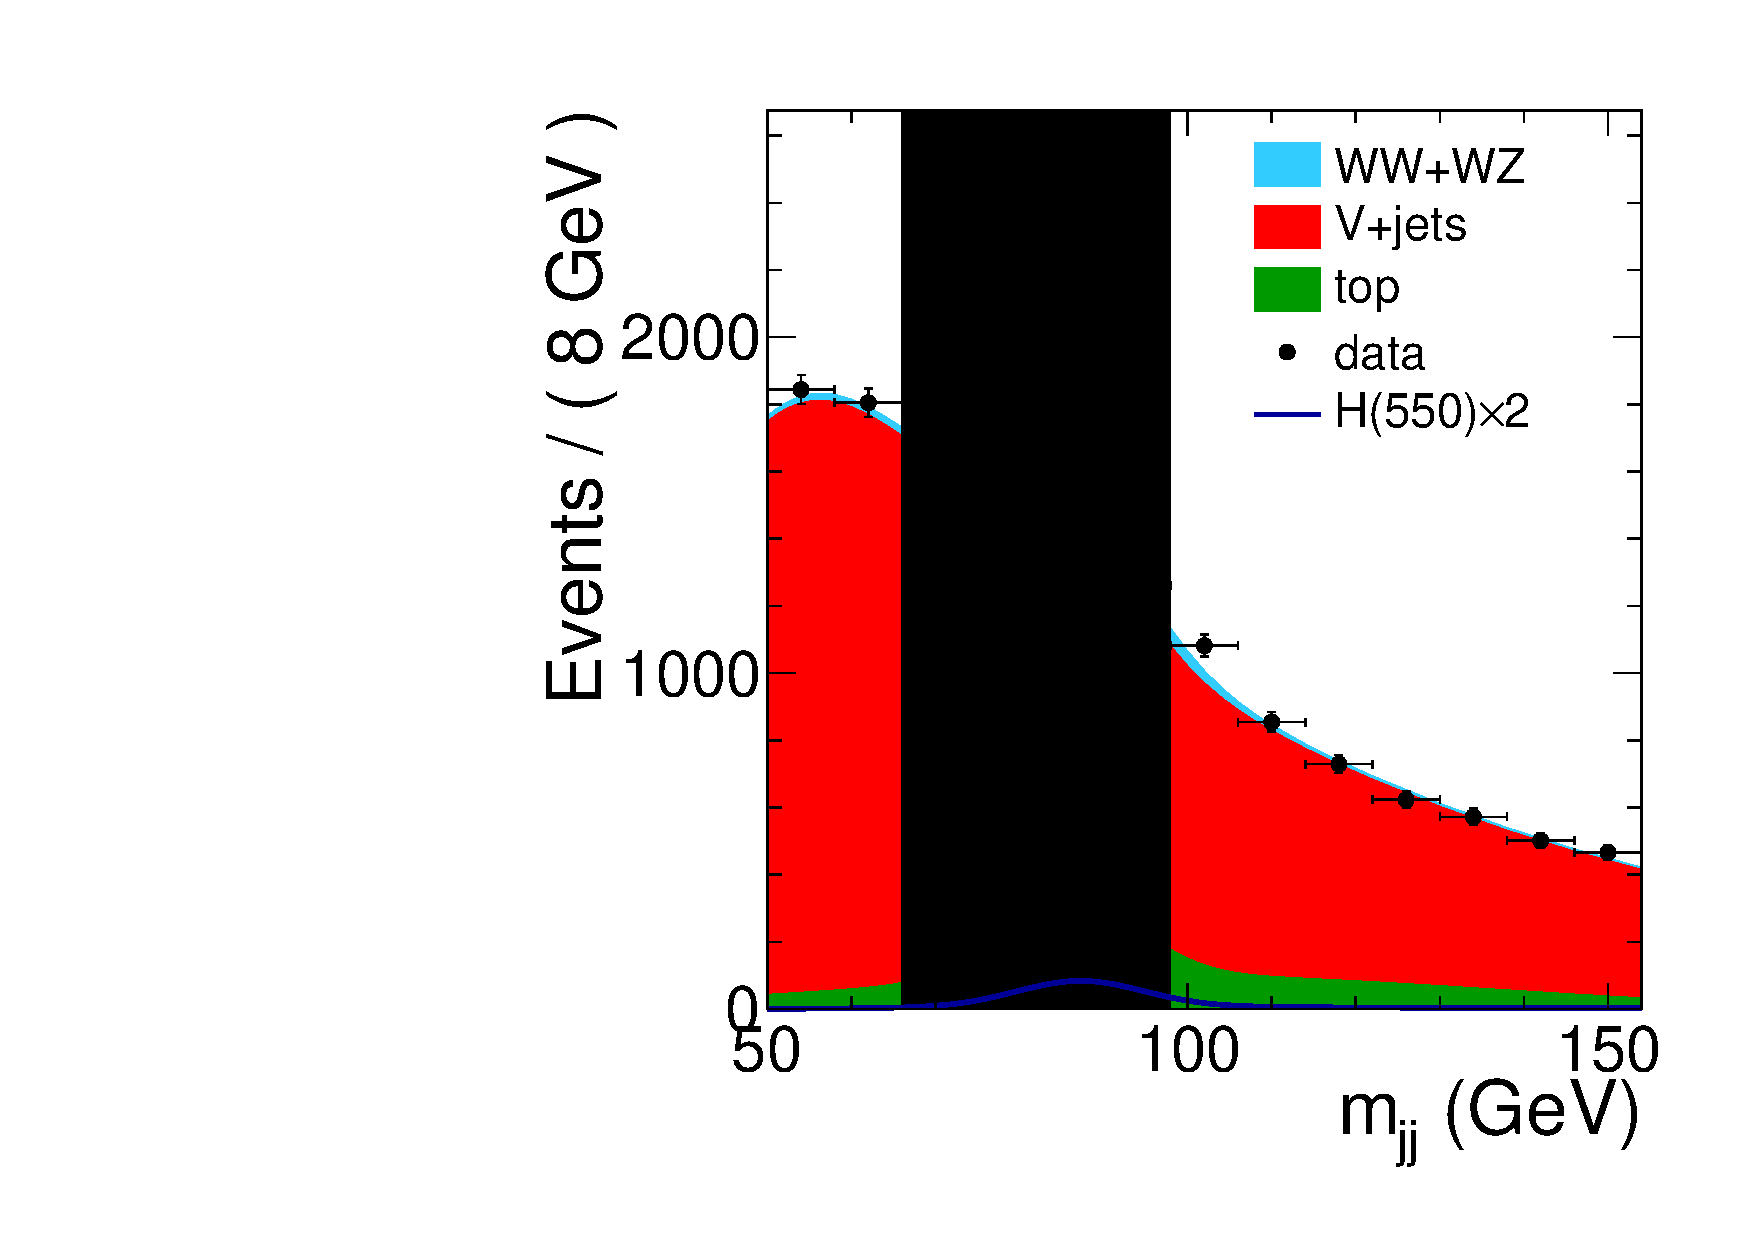
\includegraphics[width=0.49\textwidth]{plots/2012_FOURBSHAPES/HWW550lnujj_electron_mjj_stacked}
  %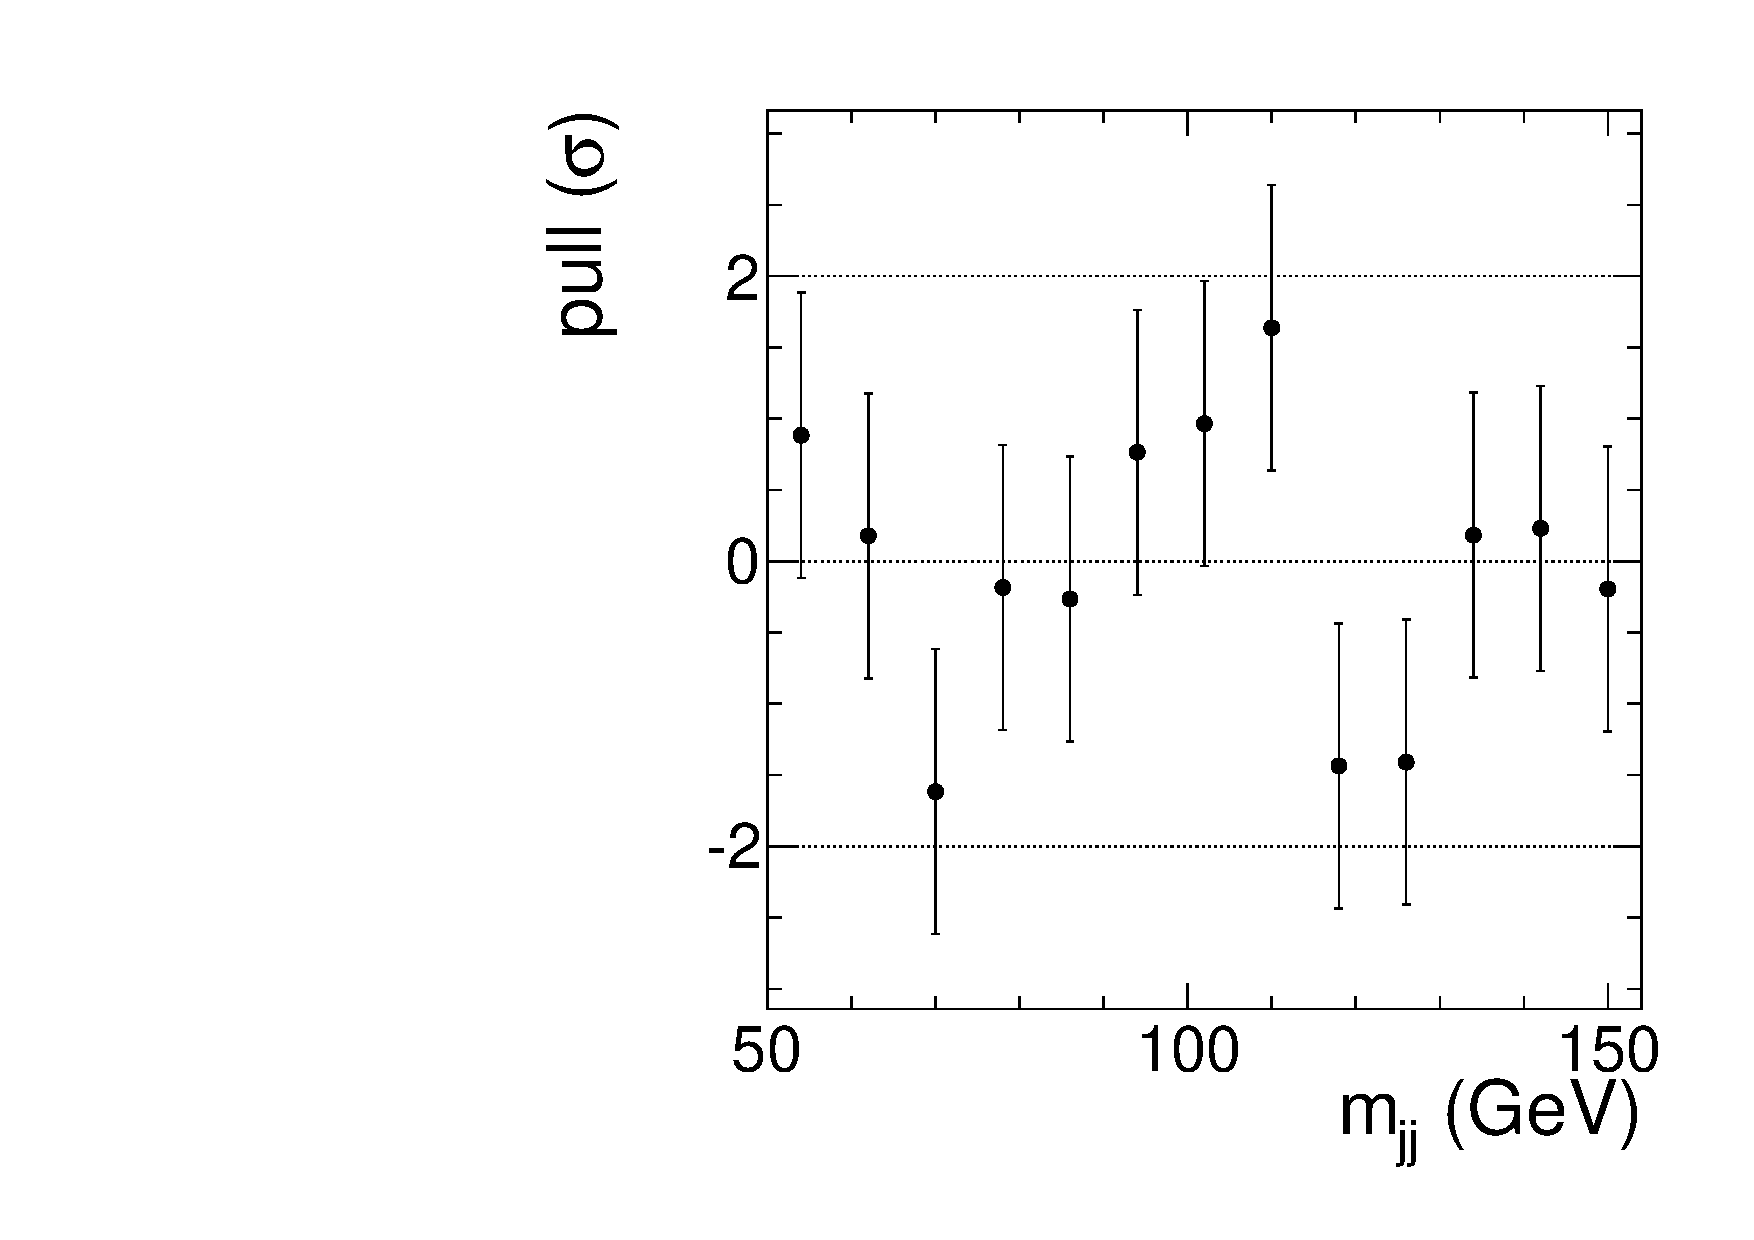
\includegraphics[width=0.49\textwidth]{plots/2012_FOURBSHAPES/HWW550lnujj_muon_mjj_pull}
  % \parbox[b][0.49\textwidth][r]{0.49\textwidth}{pull to be included when unblinded.}
  \caption{\label{fig:mjj_mH550}For the SM Higgs mass of 550~GeV, the
    distribution of the dijet invariant mass $m_{jj}$ is shown with
    muons on the left and electrons on the right.}
  % The pull
  %   distribution computed as [(Data - Fit)/ Fit uncertainty] is shown
  %   on the right. } %% The signal region is blinded.}
\end{figure}

\begin{figure}[!t]
  \centering
  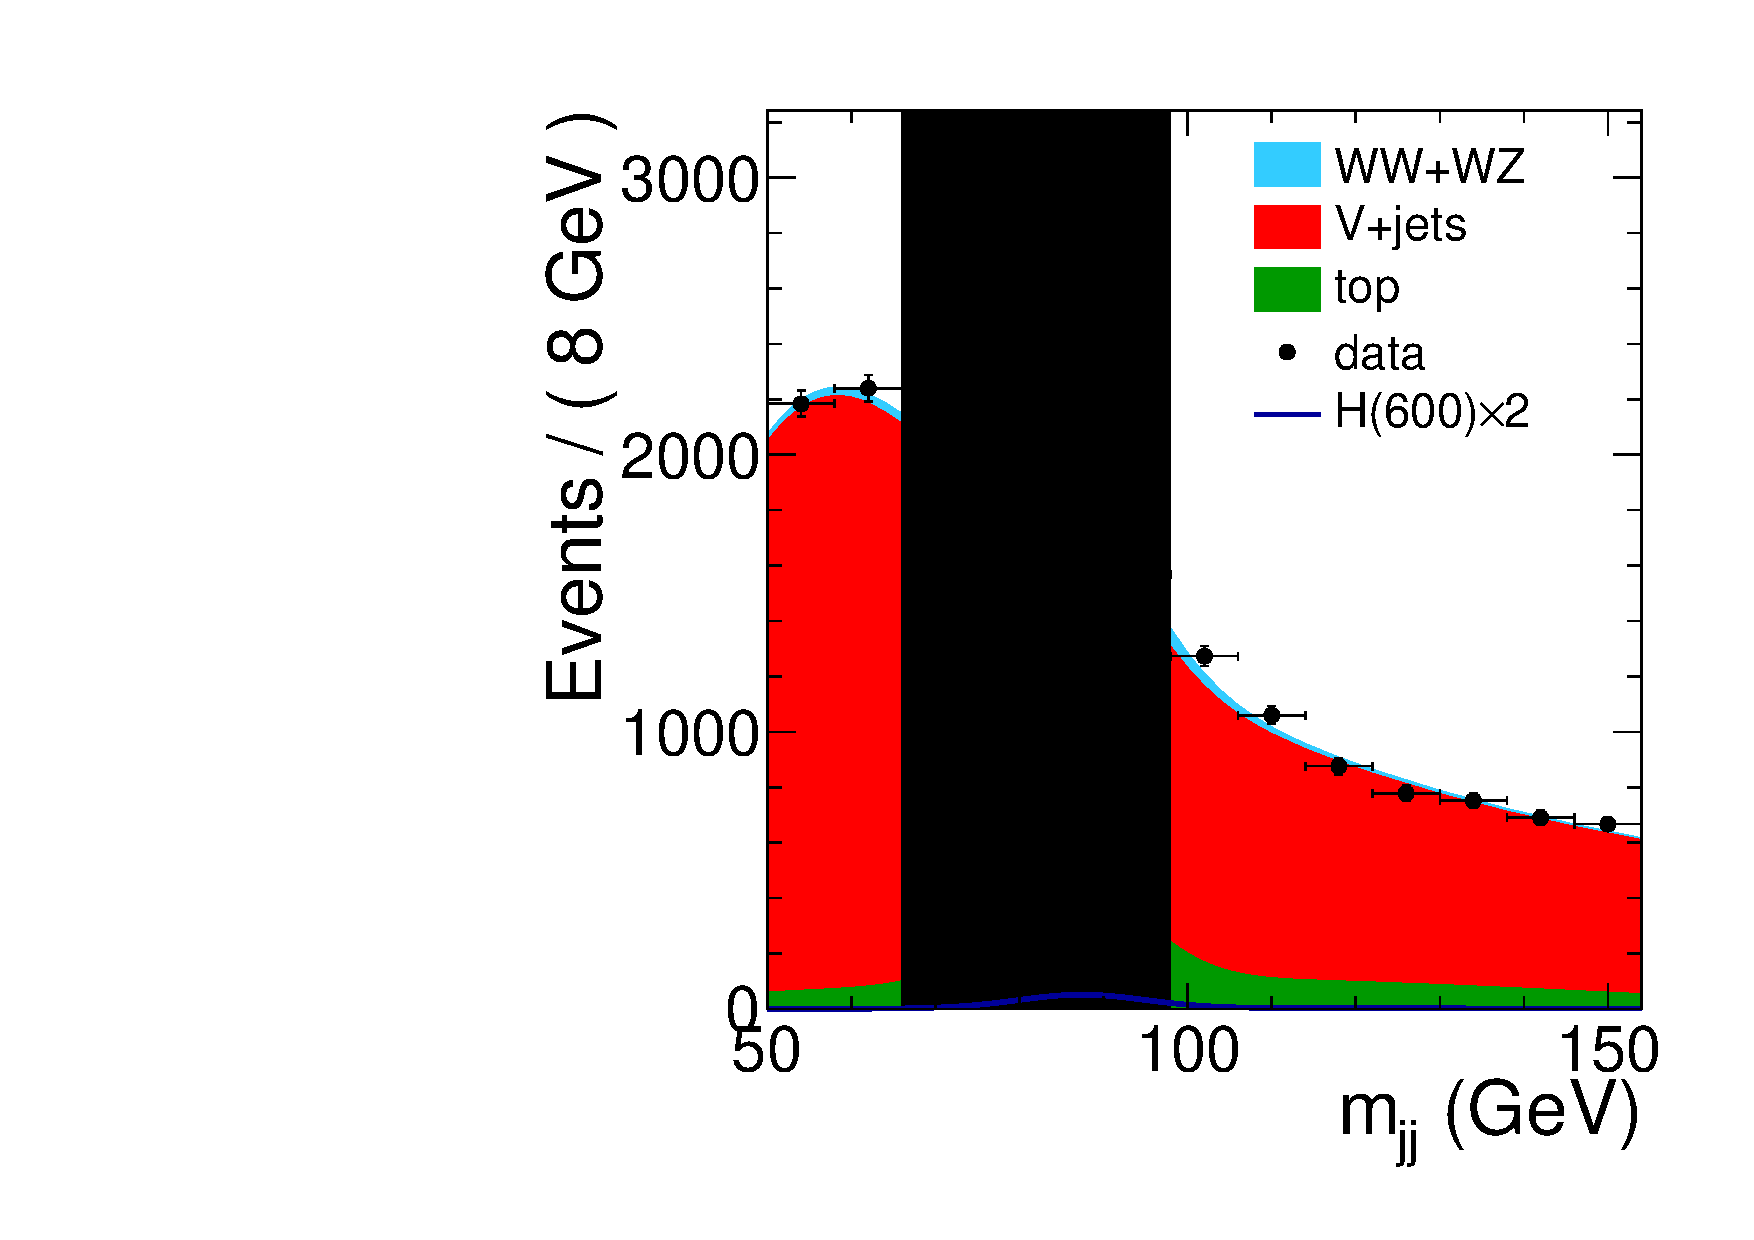
\includegraphics[width=0.49\textwidth]{plots/2012_FOURBSHAPES/HWW600lnujj_muon_mjj_stacked}
  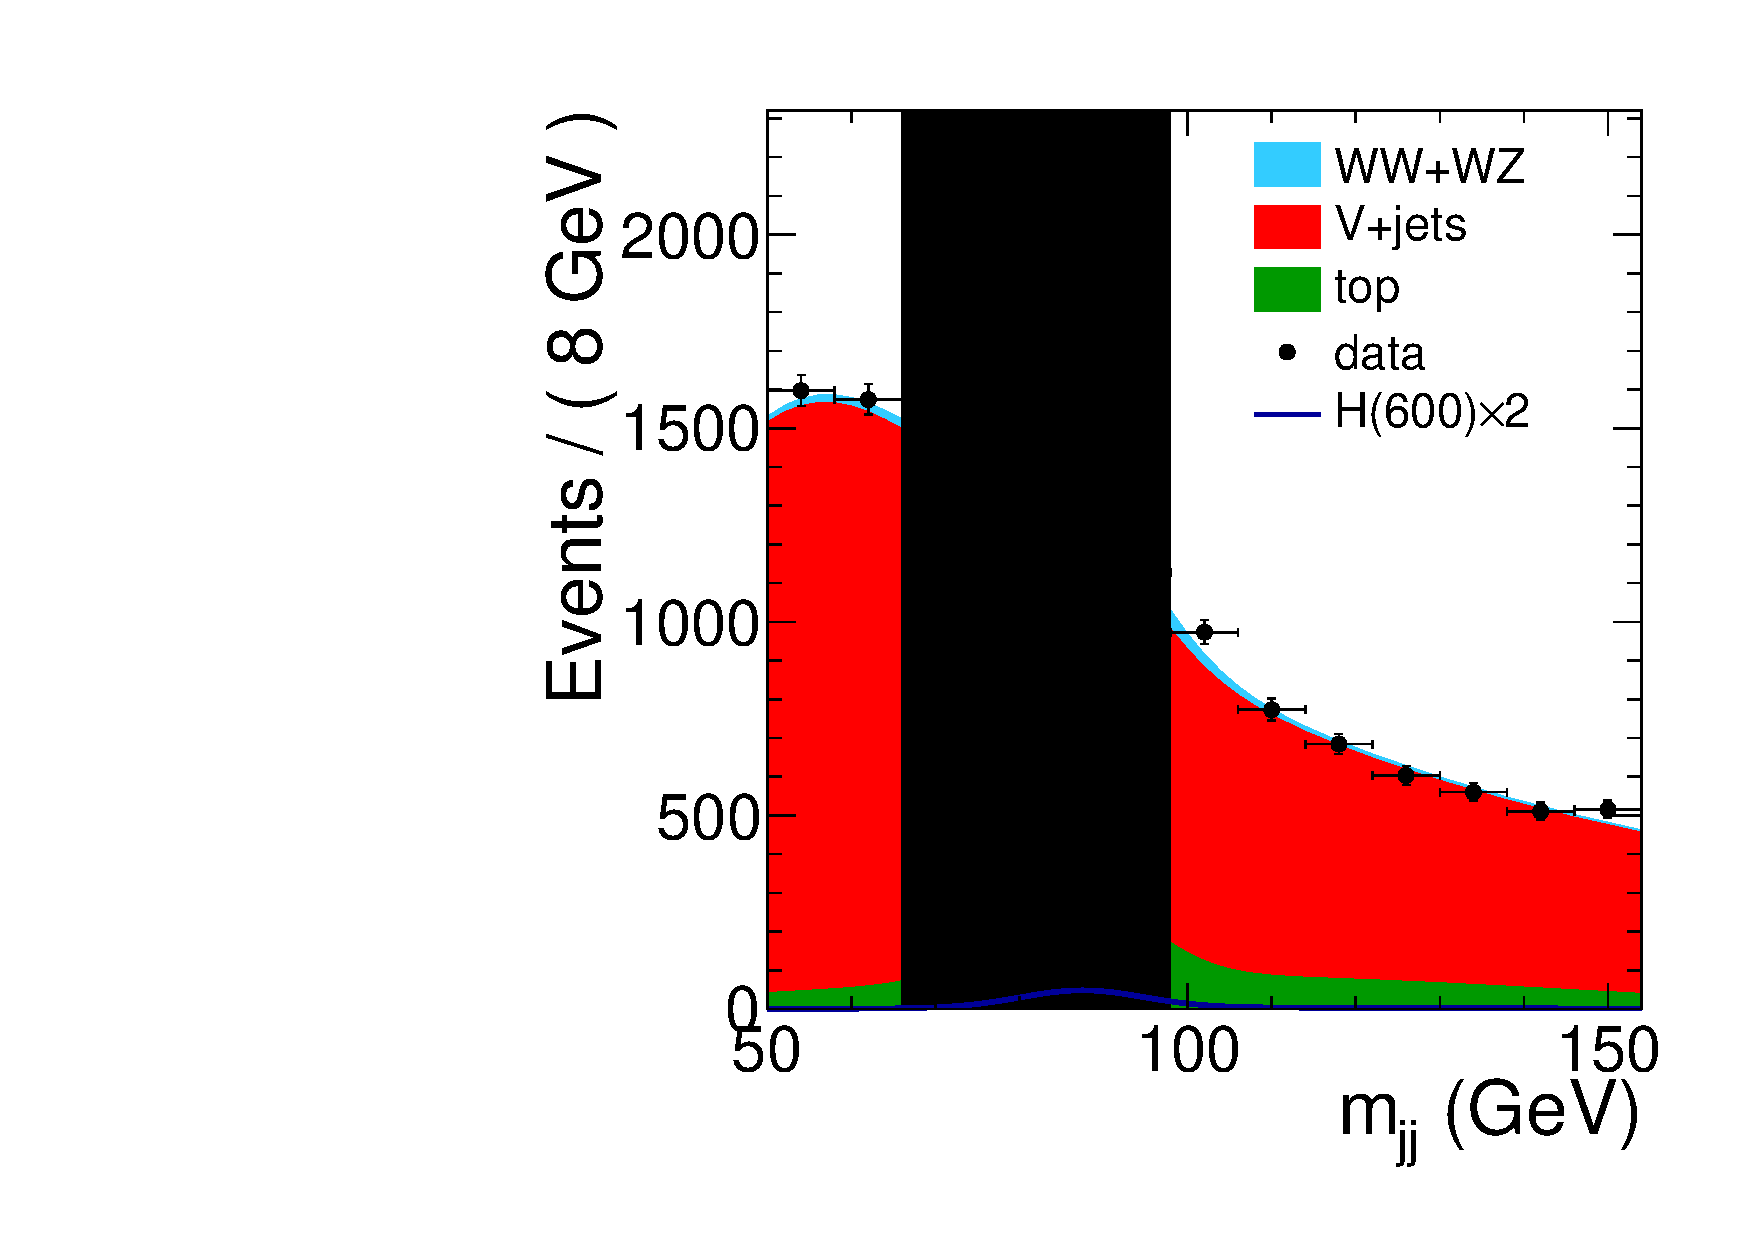
\includegraphics[width=0.49\textwidth]{plots/2012_FOURBSHAPES/HWW600lnujj_electron_mjj_stacked}
  %\includegraphics[width=0.49\textwidth]{plots/2012_FOURBSHAPES/HWW600lnujj_muon_mjj_pull}
  % \parbox[b][0.49\textwidth][r]{0.49\textwidth}{pull to be included when unblinded.}
  \caption{\label{fig:mjj_mH600}For the SM Higgs mass of 600~GeV, the
    distribution of the dijet invariant mass $m_{jj}$ is shown with
    muons on the left and electrons on the right.}
  % The pull
  %   distribution computed as [(Data - Fit)/ Fit uncertainty] is shown
  %   on the right. } %% The signal region is blinded.}
\end{figure}

\clearpage

\subsection{Use of four-body mass to extract Higgs limits}
\label{sec:mlvjjforlimit}

The four-body mass background distributions in the signal regions
after the ML fit to the data under the background only hypothesis are
shown in
Figures~\ref{fig:m4_dd_example170}-\ref{fig:m4_dd_example600}.
%%The data in the signal region is blinded/not shown.

\begin{figure}[!b]
  \centering
  \includegraphics[width=0.45\textwidth]{plots/2012_FOURBSHAPES/HWW170lnujj_muon_mWW_stacked}
  \includegraphics[width=0.45\textwidth]{plots/2012_FOURBSHAPES/HWW170lnujj_electron_mWW_stacked}

  \caption{The four-body mass distribution of data-driven background
    events in the signal regions for Higgs mass hypothesis point
    M=170~GeV.  The left plot is for the muons; the right is for
    electrons.}
  \label{fig:m4_dd_example170}
\end{figure}

\begin{figure}[!b]
  \centering
  \includegraphics[width=0.45\textwidth]{plots/2012_FOURBSHAPES/HWW180lnujj_muon_mWW_stacked}
  \includegraphics[width=0.45\textwidth]{plots/2012_FOURBSHAPES/HWW180lnujj_electron_mWW_stacked}

  \caption{The four-body mass distribution of data-driven background
    events in the signal regions for Higgs mass hypothesis point
    M=180~GeV.  The left plot is for the muons; the right is for
    electrons.}
  \label{fig:m4_dd_example180}
\end{figure}

\begin{figure}[!b]
  \centering
  \includegraphics[width=0.45\textwidth]{plots/2012_FOURBSHAPES/HWW190lnujj_muon_mWW_stacked}
  \includegraphics[width=0.45\textwidth]{plots/2012_FOURBSHAPES/HWW190lnujj_electron_mWW_stacked}

  \caption{The four-body mass distribution of data-driven background
    events in the signal regions for Higgs mass hypothesis point
    M=190~GeV.  The left plot is for the muons; the right is for
    electrons.}
  \label{fig:m4_dd_example190}
\end{figure}

\begin{figure}[!b]
  \centering
  \includegraphics[width=0.45\textwidth]{plots/2012_FOURBSHAPES/HWW200lnujj_muon_mWW_stacked}
  \includegraphics[width=0.45\textwidth]{plots/2012_FOURBSHAPES/HWW200lnujj_electron_mWW_stacked}

  \caption{The four-body mass distribution of data-driven background
    events in the signal regions for Higgs mass hypothesis point
    M=200~GeV.  The left plot is for the muons; the right is for
    electrons.}
  \label{fig:m4_dd_example200}
\end{figure}

\begin{figure}[!b]
  \centering
  \includegraphics[width=0.45\textwidth]{plots/2012_FOURBSHAPES/HWW250lnujj_muon_mWW_stacked}
  \includegraphics[width=0.45\textwidth]{plots/2012_FOURBSHAPES/HWW250lnujj_electron_mWW_stacked}

  \caption{The four-body mass distribution of data-driven background
    events in the signal regions for Higgs mass hypothesis point
    M=250~GeV.  The left plot is for the muons; the right is for
    electrons.}
  \label{fig:m4_dd_example250}
\end{figure}

\begin{figure}[!b]
  \centering
  \includegraphics[width=0.45\textwidth]{plots/2012_FOURBSHAPES/HWW300lnujj_muon_mWW_stacked}
  \includegraphics[width=0.45\textwidth]{plots/2012_FOURBSHAPES/HWW300lnujj_electron_mWW_stacked}

  \caption{The four-body mass distribution of data-driven background
    events in the signal regions for Higgs mass hypothesis point
    M=300~GeV.  The left plot is for the muons; the right is for
    electrons.}
  \label{fig:m4_dd_example300}
\end{figure}

\begin{figure}[!b]
  \centering
  \includegraphics[width=0.45\textwidth]{plots/2012_FOURBSHAPES/HWW350lnujj_muon_mWW_stacked}
  \includegraphics[width=0.45\textwidth]{plots/2012_FOURBSHAPES/HWW350lnujj_electron_mWW_stacked}

  \caption{The four-body mass distribution of data-driven background
    events in the signal regions for Higgs mass hypothesis point
    M=350~GeV.  The left plot is for the muons; the right is for
    electrons.}
  \label{fig:m4_dd_example350}
\end{figure}

\begin{figure}[!b]
  \centering
  \includegraphics[width=0.45\textwidth]{plots/2012_FOURBSHAPES/HWW400lnujj_muon_mWW_stacked}
  \includegraphics[width=0.45\textwidth]{plots/2012_FOURBSHAPES/HWW400lnujj_electron_mWW_stacked}

  \caption{The four-body mass distribution of data-driven background
    events in the signal regions for Higgs mass hypothesis point
    M=400~GeV.  The left plot is for the muons; the right is for
    electrons.}
  \label{fig:m4_dd_example400}
\end{figure}

\begin{figure}[!b]
  \centering
  \includegraphics[width=0.45\textwidth]{plots/2012_FOURBSHAPES/HWW450lnujj_muon_mWW_stacked}
  \includegraphics[width=0.45\textwidth]{plots/2012_FOURBSHAPES/HWW450lnujj_electron_mWW_stacked}
  \includegraphics[width=0.45\textwidth]{plots/2012_FOURBSHAPES/HWW450lnujj_muon_mWW_stacked_log}
  \includegraphics[width=0.45\textwidth]{plots/2012_FOURBSHAPES/HWW450lnujj_electron_mWW_stacked_log}

  \caption{The four-body mass distribution of data-driven background
    events in the signal regions for Higgs mass hypothesis point
    M=450~GeV.  The left plot is for the muons; the right is for
    electrons.  The bottom set of plots is the same plot with a log
    scale rather than linear.}
  \label{fig:m4_dd_example450}
\end{figure}

\begin{figure}[!b]
  \centering
  \includegraphics[width=0.45\textwidth]{plots/2012_FOURBSHAPES/HWW500lnujj_muon_mWW_stacked}
  \includegraphics[width=0.45\textwidth]{plots/2012_FOURBSHAPES/HWW500lnujj_electron_mWW_stacked}
  \includegraphics[width=0.45\textwidth]{plots/2012_FOURBSHAPES/HWW500lnujj_muon_mWW_stacked_log}
  \includegraphics[width=0.45\textwidth]{plots/2012_FOURBSHAPES/HWW500lnujj_electron_mWW_stacked_log}

  \caption{The four-body mass distribution of data-driven background
    events in the signal regions for Higgs mass hypothesis point
    M=500~GeV.  The left plot is for the muons; the right is for
    electrons.  The bottom set of plots is the same plot with a log
    scale rather than linear.}
  \label{fig:m4_dd_example500}
\end{figure}

\begin{figure}[!b]
  \centering
  \includegraphics[width=0.45\textwidth]{plots/2012_FOURBSHAPES/HWW550lnujj_muon_mWW_stacked}
  \includegraphics[width=0.45\textwidth]{plots/2012_FOURBSHAPES/HWW550lnujj_electron_mWW_stacked}
  \includegraphics[width=0.45\textwidth]{plots/2012_FOURBSHAPES/HWW550lnujj_muon_mWW_stacked_log}
  \includegraphics[width=0.45\textwidth]{plots/2012_FOURBSHAPES/HWW550lnujj_electron_mWW_stacked_log}

  \caption{The four-body mass distribution of data-driven background
    events in the signal regions for Higgs mass hypothesis point
    M=550~GeV.  The left plot is for the muons; the right is for
    electrons.  The bottom set of plots is the same plot with a log
    scale rather than linear.}
  \label{fig:m4_dd_example550}
\end{figure}

\begin{figure}[!b]
  \centering
  \includegraphics[width=0.45\textwidth]{plots/2012_FOURBSHAPES/HWW600lnujj_muon_mWW_stacked}
  \includegraphics[width=0.45\textwidth]{plots/2012_FOURBSHAPES/HWW600lnujj_electron_mWW_stacked}
  \includegraphics[width=0.45\textwidth]{plots/2012_FOURBSHAPES/HWW600lnujj_muon_mWW_stacked_log}
  \includegraphics[width=0.45\textwidth]{plots/2012_FOURBSHAPES/HWW600lnujj_electron_mWW_stacked_log}

  \caption{The four-body mass distribution of data-driven background
    events in the signal regions for Higgs mass hypothesis point
    M=600~GeV.  The left plot is for the muons; the right is for
    electrons.  The bottom set of plots is the same plot with a log
    scale rather than linear.}
  \label{fig:m4_dd_example600}
\end{figure}

%The full set of plots for the analysis on the 48 working points can be
%found in the CMS analysis note AN-2012/024, Section 15.

\clearpage
